% arara: xelatex: { shell : yes }
% arara: biber
% arara: xelatex: { shell : yes }
% arara: xelatex: { synctex: 1, shell : yes }

\documentclass[thesis=M,english]{template/FITthesis}[2019/12/23]
\usepackage[utf8]{inputenc} % LaTeX source encoded as UTF-8
\usepackage{dirtree}
\usepackage{xevlna}
\usepackage{hyperref}
\usepackage{caption}
\usepackage{enumitem}
\usepackage{booktabs}
\usepackage{multirow}
\usepackage{tabularx}
\usepackage{blindtext}

\makeatletter
\newcommand\my@hyphen{-}
\newcommand\my@apostroph{'}
\patchcmd\select@language{-}{\my@hyphen }{}{\fail}
\patchcmd\select@language{'}{\my@apostroph }{}{\fail}
\makeatother

\usepackage[style=iso-numeric,backend=biber]{biblatex}
\addbibresource{library.bib}

\usepackage{minted}
\counterwithin{listing}{chapter}
%\renewcommand{\listingscaption}{Výpis kódu}
%\renewcommand{\listoflistingscaption}{Seznam výpisů kódu}

\usepackage{lineno}
\usepackage{csquotes}
\usepackage{placeins}
\usepackage{suffix}

\usepackage{xcolor} 
\newcommand{\todo}[1]{\textcolor{red}{\textbf{[[ #1 ]]}}}

\usepackage{blindtext}
\newcommand{\blind}[1][1]{\textcolor{lightgray}{\blindtext[#1]}}

\newcommand*{\myAppName}{King Karel}

% Item for Enumerate that feels like Subsection.
%
% 1 - description

\newcommand{\myItem}[1]{\item{\textbf{#1} --}}
\WithSuffix\newcommand\myItem*[1]{\item[\refstepcounter{enumi}(*\number\value{enumi})]{xyz \textbf{#1} --}}

% Additional commands for quotes.

% Czech simple quotes.
\newcommand{\juv}[1]{,#1`}

% Czech side quotes quotes.
\newcommand{\buv}[1]{>>#1<<}

% English quotes.
\newcommand{\auv}[1]{``#1''}

% English simple quotes.
\newcommand{\ajuv}[1]{`#1'}



% % % % % % % % % % % % % % % % % % % % % % % % % % % % % % 
% SETTINGS
% % % % % % % % % % % % % % % % % % % % % % % % % % % % % % 

\department{Department of Software Engineering}
\title{King Karel -- An~Educational Programming Puzzle Game}
\authorGN{Jan} %(křestní) jméno (jména) autora
\authorFN{Bittner} %příjmení autora
\authorWithDegrees{Bc. Jan Bittner} %jméno autora včetně akademických titulů
\author{Jan Bittner} %jméno autora bez akademických titulů
\supervisor{Ing. Jan Matoušek}
\acknowledgements{Throughout the~writing of this thesis I~have received a~great deal of support and assistance.
\\\\
First and foremost,
I~would like to express my deep gratitude to my~supervisor,
Ing.~Jan Matoušek.
I~am incredibly grateful for our friendly chats
and his dedicated support and guidance.
\\\\
I~want to acknowledge my colleagues from the~FIT Discord community for their tremendous support throughout my studies.
Their regular dose of memes often improved my mood.
It has been an~honor to serve beside you.
\\\\
Last but not least,
I~owe more than thanks to my family and friends
for providing me with unfailing support and continuous encouragement throughout my years of study and through the~process of writing this thesis. This accomplishment would not have been possible without them. Thank you.
}
\abstractCS{Magisterská práce se zabývá vývojem prototypu hry King Karel,
logické hry na výuku programování.
Práce popisuje proces analýzy, návrhu a~implementace zmiňované hry s důrazem na návrh architektury jednotlivých částí.
Klientská část je tvořena pomocí frameworku Flutter a~serverová část je tvořena pomocí frameworku ASP.NET Web API.
}
\abstractEN{The~master's thesis deals with the~development of a~prototype of the~game King Karel~--
an educational programming puzzle game.
The~thesis describes the~process of analysis, design, and implementation of the~mentioned game,
emphasizing the~design of the~architecture of individual parts.
The~client part is created using the~Flutter framework,
and the~server part is created using the~ASP.NET Web API framework.
}
\placeForDeclarationOfAuthenticity{Prague}
\declarationOfAuthenticityOption{2} %volba Prohlášení
\keywordsCS{výuková hra, web, desktop, Flutter, C\#, programovací\linebreak{}logická hra, multiplatformní framework}
\keywordsEN{educational game, web, desktop, Flutter, C\#, programming puzzle, cross-platform framework}
\website{https://github.com/tenhobi/masters-thesis} %volitelná URL práce, objeví se v tiráži

% % % % % % % % % % % % % % % % % % % % % % % % % % % % % % 
% OBSAH
% % % % % % % % % % % % % % % % % % % % % % % % % % % % % %  

\begin{document}
\overfullrule=30pt

\begin{introduction}

In recent years people have used more and more games and applications, mainly due to the~arrival, further development, and massive popularization of laptops, mobile phones, and other smart devices.

For clarity, this thesis uses the~term \emph{game} for a~type of a program whose purpose is to entertain or use the~user's knowledge to elevate the mechanics of the~game in comparison with the~term \emph{application} for a~type of a program whose primary purpose is helping a~user do things.
Therefore even though regular users might refer to some programs as applications, the~term game will be used instead in this thesis.

Although not many games design their concepts to be educational, the~benefits of educational aspects are crystal clear.
It is always good to introduce as many fun concepts and mechanics as possible for educational applications.

Dedicated educational games introduce students to the~studied subject using classical approaches such as strictly focusing on the~topic with no extra features.
While using interactive methods fulfills its purpose, and students can learn the~concepts from these resources, they also face problems with students' attention spans because they feel bored with the~knowledge they are learning.

Instead of developing only dull and bland dedicated educational applications, many games use a~concept called \emph{gamification}.
Gamification is a~relatively new technique without a~clear definition.

According to the~article~\cite{dichev_2017_gamifying}, gamification in education is a~psychologically driven approach to increasing the~motivation and engagement of students by including game design principles.
The~article also states that research on gamification is diverse and that the~focus is mainly on empirical studies. However, the~article also \textquote{identified a~growing number of studies reporting empirical evidences for the~effectiveness of gamification in educational context.}
It also states that the~understanding of gamification processes is limited, and it is unknown how to produce beneficial learning outcomes while avoiding harmful learning outcomes. 

According to the~article~\cite{smiderle_2020_the}, gamification might affect participants differently based on their personality traits.
The~study used students from an~undergraduate programming class who were given gamified and non-gamified learning environments.
The~article concludes that students with low agreeableness, low openness, and introverts showed remarkable improvement and that introverted students were more engaged than extroverted ones.

In the~article~\cite{nand_2019_engaging} the~study examines the~effects of gamification on numeracy at a~primary school level.
They selected three features from the~survey~-- challenges, feedback, graphics~-- and created two game versions presented to children.
One with all features enabled and the~second one with an~apparent lack of these features.
The~results showed that gamification methods were \textquote{more effective in enhancing children's learning and they found it more engaging.}

After reviewing mentioned articles, it is clear that gamification in education has been proven by empirical methods to provide a~significantly better and more engaging learning environment.
Mentioned studies show a~good direction in designing an~entertaining education game despite the~lack of non-empirical studies on psychological benefits.

\section{Motivation}

I have enjoyed playing computer games from an early age.
Although most of my friends exclusively played non-educational games or games where one did not need to think, I always enjoyed the puzzle, strategic, building, and educational games.
Even today, I remember how I and my sister both played together game \emph{Alík - Veselá matematika} to practice the basics of mathematics.
This game was enjoyable, even though it was an educational game.
The main reason was that it had some story, and it did not feel like learning.
It felt like playing a video game.
You needed to compute some numbers to move or help some character in the game.
After completing a task, you receive some points, and I think using them, you could acquire some toys for your in-game collection.

These concepts sound like gamification to me, and I would like to create a prototype for a game that will teach children the basics of programming concepts, so maybe some children, like me years prior, will enjoy their time learning a bit more.

I have been helping with organizing summer camps and other events for children with a local organization for years.
We prepare activities and games for children to enjoy the time and learn something new.
I also have experience educating children and adults while writing technical articles and lecturing about programming.
I always try to present relevant information in the most friendly form in all my articles and lectures.
In the future, I would like to focus on developing an educational project or teaching.

\section{Aims and Objectives}

Gamification in education is a~noteworthy aid to educational games.
This thesis focuses on the~analysis, design, and development of a~prototype of such a~game
that focuses on teaching programming concepts.

Due to mentioned motivations, the~game is aimed primarily at young people, but this condition is not exclusive; everyone will be able to play the~game.
That means focusing on middle school or high school children, i.e., 11 to 18 years old.
Therefore, the~game must be simple, easy to understand, and the~mechanics shall be quick to master.

In order for the~game to be designed as best as possible, a~survey among children, parents, and teachers will be needed.
Based on the~survey and the~mentioned articles, an~analysis of the~requirements for the~game will be created.
Then the~game will be designed and implemented, and finally, usability testing will be performed and evaluated.


\end{introduction}

%
%
\chapter{Survey}
\label{survey}

Surveys gather information through questions on a~sample of people.
They can take many forms, including telephone surveys, face-to-face surveys, paper surveys, and online surveys.
Unlike other forms, online surveys benefit from being faster, cheaper, more accurate, and easy to get and analyze.

Online surveys often consist of open-ended and closed-ended questions that help analyze the~studied topic.
They can also contain different questions based on participants' roles.
There are also dedicated applications to create and conduct online surveys that can set up different questions, separate them into individual groups or pages, make conditions to display them only to specific user roles, etc.

The~first important task is defining the~survey's goals and who to survey.
With that in mind, questions are created.
And in the~end, the~gathered data has to be analyzed.
It is often required to process and adjust the~data before analyzing, especially the~open-ended questions.
Therefore a~human worker must go through these questions and take out the~relevant data.

\section{Conducted Survey}

Even though this thesis focuses on developing a prototype mainly focused on children, also parents and teachers participated in it.
The game's future development counts on developing more features to include these user groups in the children's education.

Articles mentioned in the introduction also analyzed some use-cases of gamification in education or educational games.
These studies have been analyzed, and the conducted survey follows and considers their results. 

The primary purpose of the conducted survey for this thesis was to understand what some children, their parents, and teachers think and would make them motivated in a gamified game.

The survey recognizes three participant roles: a child, a parent, and a teacher.
Each role has a modified set of questions.

\subsection*{Questions asked only to children}

\begin{enumerate}
    \item What (non-educational) games do you usually play and why? What is your motivation for playing them? (Open-ended question.)
    \item Do you like receiving points as a reward for completing tasks? (Closed-ended question.)
    \item Do you like rankings in educational games? (Closed-ended question.)
    \item Would you like an advanced final task as a challenge? (Closed-ended question.)
    \item What is your primary motivation to play an educational game? (Open-ended question.)
\end{enumerate}

\subsection*{Questions asked to children, parents, and teachers}

\begin{enumerate}
    \item What aspects or mechanics are important in an educational game according to you? ((Closed-ended question with options: a game; a story; study materials; an explanation.)
    \item Do you (or your children/students) use any educational application or game? (Closed-ended question with options: Duolingo, Khan Academy, Minecraft, Scratch, other.)
    \item What experiences do you have with educational applications or games. What aspects do you like the most, what don't you like? (Open-ended question.)
    \item What would you appreciate most in an educational game? (Open-ended question.) 
\end{enumerate}

\subsection*{Questions asked only to parents and teachers}

\begin{enumerate}
    \item What is important to you? (Closed-ended question with options: progress monitoring; checking the results; ratings and comparison with other players; planning tasks for children to practice; an option to change child's settings.) 
\end{enumerate}

\section{Evaluation}

The~survey where children, parents, and teachers participated was held online using Google Forms.
An equivalent face-to-face survey was also done with children.
Both groups showed, on average, the~same results.

The~assumptions before doing the~survey were that at least 90 percent of respondents play non-educational games;
respondents (especially children) play some building games (such as Minecraft), children are mostly (at least 75 percent) competitive, and the~most crucial aspect is the~game itself, explanation, and a~story.

The~survey results pointed out that almost 22 percent of respondents do not play non-educational games.
Almost 18 percent of respondents (primarily children) play building games.
Respondents also chose to play casual games and shooting games in almost 14 percent of responses, puzzle or strategy games in nearly 12 percent of responses, board games, battle-royal-like games, and shooting games in about 7 percent.
The~results of which non-educational games people play are shown in figure~\ref{fig:survey:games}.

\begin{figure}
    \centering
    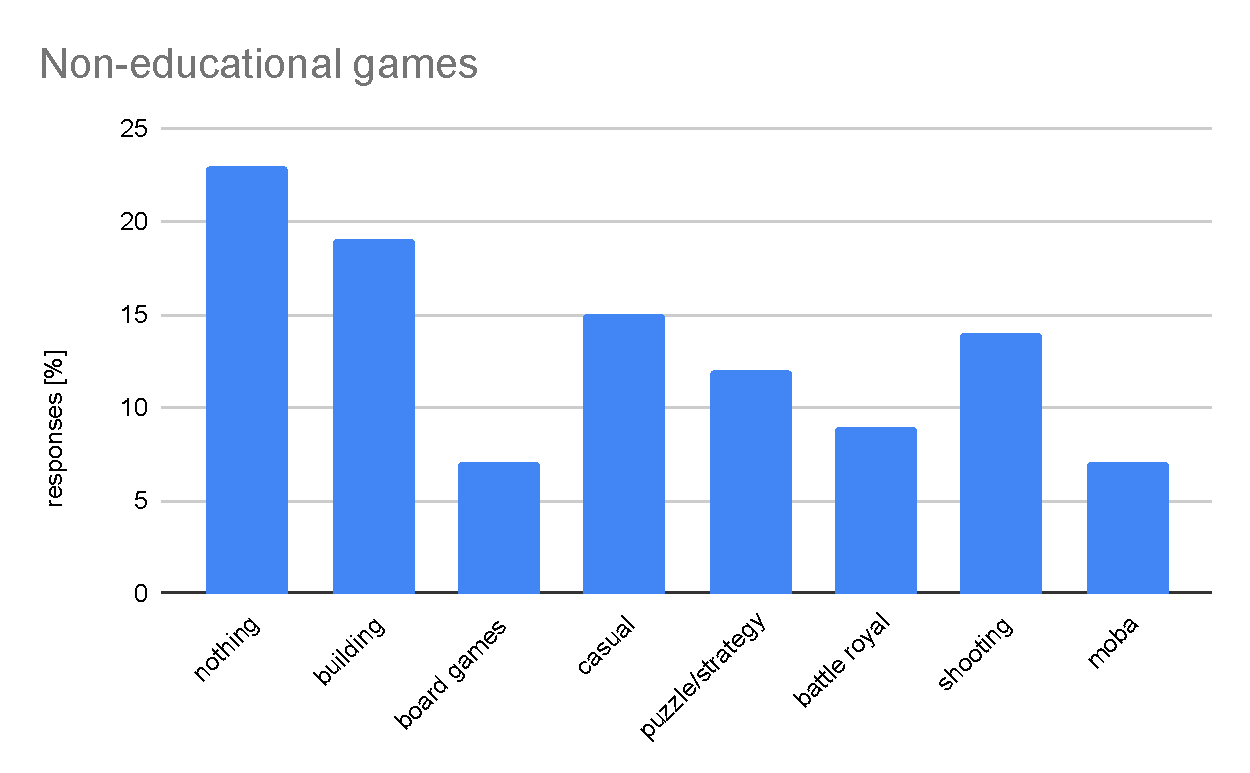
\includegraphics[width=1\linewidth]{assets/survey/non-educational-games.pdf}
    \caption{Played Non-educational Types of Games}
    \label{fig:survey:games}
\end{figure}

In a~matter of educational games people use, almost 60 percent of respondents use Duolingo~-- language learning educational game.
Almost 30 percent of respondents also selected Minecraft~-- a~game known for its building mechanics and an~option to program with unique blocks.
Almost 15 percent of respondents use Scratch~-- a~tool to do visual programming.
Other minor answers were, for example, Khan Academy and Kahoot with almost 7 percent.  

Focusing on children's answers, almost 80 percent like receiving some reward for completing tasks; nearly 75 percent like rating systems; and almost 80 percent of respondents would like the~last task to be a~challenge.

Questions about what aspects or mechanics are important in an~educational game showed exciting differences.
While children selected with the~same share a~game, a~story, and an~explanation, almost none selected study materials.
Parents and teachers selected a~story and an~explanation, while almost none chose a~game and study materials.
Interestingly, the~difference between children and parents or teachers is the~view on the~importance of the~game aspects.

The~results and initial assumptions contradict that most people play non-educational games; confirm that building games are the~most common kind of games children play; and show that children are~-- majority with almost 75 percent~-- competitive. 

The~conducted survey with the~addition of articles mentioned in the~introduction suggests that gamification in educational games might introduce valuable benefits.
In summary, children like to receive rewards in some form of points, want to compete and be rated, and like challenges.
All these factors underline the~motivational aspects found in mentioned studies,
as they help to increase the~attention span.


\chapter{Analysis}
\label{analysis}

According to previous chapters' survey results and other resources, this chapter describes the~game's prototype analysis.
The~output of this chapter is an~analysis of the~game's concepts, mechanics, and screens and setting functional and non-functional requirements.

\section{Analysis of the Game}
\label{analysis:game}

The game \emph{\myAppName} is an educational programming puzzle game that uses gamification methods to enhance its capabilities in educating children's programming concepts.

The game should be accessible to a majority of users.
Therefore it should be provided as a web and desktop application.
These game versions should be equal in features, look-alike, and have the same synced content.
Additionally, the game should be prepared for expanding to mobile devices, either using responsive web technologies or as dedicated programs.

\subsection{Stories and Missions}
\label{analysis:game:stories-and-missions}

The game is built around the stories of Karel, the king, who must solve the problems plaguing his land and other adventures.
In the stories, Karel must complete tasks and fight difficulties using the proper use of algorithms.
He can move, put and grab marks, look around and determine if he should do some action or he can repeat them.
He also has to be careful not to step into the woods, a lake, a wall, or outside his land.
Making the game around stories should increase motivation to play, as suggested by conducted survey and mentioned articles.
It is also an excellent way to connect game missions with storytelling and learning missions.

Each story contains several missions.
Each mission can be focused on storytelling, learning, or playing.
As the player continues through the story,
they learn new concepts and practice the skills by helping the king with his tasks.
Storytelling missions aim to increase motivation to play because players will be motivated to learn about the characters.
Learning missions aim to introduce players to new concepts or explain what they can use in the game or how games evaluate their competition.
Game missions aim to provide players with a fun aspect.
The game challenges players, who have to think, but their focus is to move or control their character, not focus on learning and practicing programming concepts.

Story selection contains a name and a description of a story and its count of missions.
Mission selection of a specific story contains its missions in order.
Each mission also contains graphics representing its type; a book for a storytelling mission, a university hat for a learning mission, and a boat for a game mission.
A game mission also contains additional statistics information in the form of crowns.
Game missions can have up to three crowns; one -- the biggest -- for completing a mission, one for meeting the size criteria, and one for completing the speed criteria.

\subsection{Game Missions}
\label{analysis:game:game-missions}

Game missions should offer multiple ways to solve a problem.
Some can be easy and almost step-by-step.
Some might be solved using loops or ifs to make the program more efficient or fast.

For the prototype purpose, an initial story and its missions are made.
Each game mission contains a game grid that shows and represents the current view of the game progress.
It also contains a description view, a command panel view with a list of commands used to program the game, a command palette, and control buttons.
Using commands, a player can alter the game, which updates the grid view, and the player can see how their character moves or does other things.
Each command is also displayed with a mark on execution, indicating that that command is in use.
Players can show or hide descriptions and reset, save, or run a game using control buttons.
While a game is in progress, players can not alter the commands, but they can stop the running game. 

There are only basic commands available for the initial story and its missions.
Those commands are \mintinline{text}{move <direction>}, to move the charakter in a direction; \mintinline{text}{put mark}, to place a mark to a current cell; \mintinline{text}{grab mark}, to pick up mark from a current cell; \mintinline{text}{if <condition>} to conditionally execute inner commands; and \mintinline{text}{while}, to conditionally loop and execute inner commands.
Used direction is initially \mintinline{text}{?}, meaning the player has to change it to a valid state.
They can choose from \mintinline{text}{up}, \mintinline{text}{right}, \mintinline{text}{down}, and \mintinline{text}{left}.
Similarly, the used condition is also initially \mintinline{text}{?}.
Players can choose from conditions \mintinline{text}{can move up}, \mintinline{text}{can move right}, \mintinline{text}{can move down}, \mintinline{text}{can move left}, \mintinline{text}{can put mark}, and \mintinline{text}{can grab mark}.

Players can pick and place commands from the command palette in the default place or into the commands' inner place if they have one.
Commands also can be reordered by drag-and-drop gestures.
The position of dragged commands has the same graphics but has half opacity.
Commands dragged out of the palette do not have a position, but their position is synced after the first pass over the default or inner places.
And they can be thrown away by dragging command away from the default or inner place.
Commands dragged out have quarter opacity to signify that the command will be removed.

As has been mentioned, the grid contains cells of different types.
Some of the cells are walkable, and some of them are non-walkable.
Walkable cells are empty, and players can put and grab marks from them.
Non-walkable cells represent natural structures like walls, lakes, or forests.
Players cannot walk to those cells; otherwise, they will throw an error.

The game mission screen shows a status dialog after a running game finishes.
The dialog is either with success or failure statuses.
The failure dialog also shows a note of which specific error occurred.
The error can represent invalid commands, invalid moves, invalid use of put-mark command, invalid use of grab-mark command, or exceeding the speed limit.

A status dialog also shows statistics of speed and size attributes.
The size attribute corresponds to the number of commands used.
The speed attribute corresponds to the number of executed commands.
They are both optional challenges for players to gain additional points.
If the game does not meet the size or speed criteria, the dialog displays that attribute in a failure color.

\subsection{Statistics}
\label{analysis:game:statistics}

Players can also show results from playing game missions.
The statistics divide its view by a story.
Each story then contains rows for each of its game missions containing a mission name, if the mission is completed, and what size and speed results they have.

\subsection{Profile}
\label{analysis:game:profile}

Players can also display their profiles to check the used username, email address, or description.
The corresponding screen should be the first screen they are introduced to after the registration.

\subsection{Signing Up, In and Out}
\label{analysis:game:sign-up-in-out}

The game has a main menu containing different buttons that control navigation between screens.
It consists of the main screen button, stories button, stats button, profile button, about-us button, and sign-out button.
If the player is not signed in, the menu contains sign-up and sign-in buttons.

To sign up, the player has to fill in the username, password, real name, email, and description text fields.
After submitting the form, either by using the submit action or by clicking the submit button, signing up is done, and if no conflicts occur, the player is redirected to their profile screen.
Similarly, the player must fill in the username and password to sign in.
If the password and username match the player's record, the player is redirected to their profile screen.
If any error occurs for both processes, a fail message is displayed.

\subsection{Game Information}
\label{analysis:game:game-information}

The game must have a space to display information about the approach, contact, guidelines, help, info, press, privacy, and terms.
It should all be on one screen or divided into connected subscreens.
These screens should be accessible from the main menu.
A small sub-menu with references to these screens should be on all screens if their design allows that.

\subsection{Future Features}
\label{analysis:game:future-features}

Not every feature can be made for the prototype version.
Therefore, other analyzed features suggested for future development are recognized in this section.

\subsubsection{Game Mission}

First, game missions will introduce more commands players can use.
One of the first features that should be implemented in the future is the feature of creating separate function-like commands.
That means that players will be able to create commands that can be reused both in the default command list, in other function-like commands, and even in the current function-like command to allow using programming constructs like recursion.
These commands will be added to the command palette in a special section.
Players will be able to update them after invoking a particular action to switch the default command list to the command's command list.

Game missions should also introduce unique cells that can contain machines.
Every machine can also add a set of commands that Karel can use, including conditions.
That means that machines can be, for example, activated or deactivated.
Interactions with machines, or their end state, can also be included in evaluating the mission.
Machine cells can be both walkable and non-walkable.
They can also share a state, so two machines can work with one logical property.

While machines are stationary cell-locked entities, tools that the game mission should also introduce are to be carried with the character.
Tools can also introduce commands, conditions, and directions.
But the use of these commands should have limited use, so they can be used only if the character carries the tool at the moment.  
Therefore, tools can be picked and placed on walkable cells or inside a machine that might destroy the item.

Tools and machines can introduce an almost unlimited number of features.
Players could, for example, use teleport, walk to different lengths of steps, open a door, deactivate a trap, and much more.
Tools or machines can also add negative perks.

Later updates of the game mission can also introduce the feature of combining tools.
For example, players will be forced first to collect two diamonds that can be combined into a diamond key that can open doors.

\subsubsection{Practice Missions}

There could also be another type of mission, practice.
This mission would check that players understand storytelling and learning missions.
Practice missions can contain a simple quiz with multiple simple yes-no or ABC quiz-like questions.

With these concepts, game missions could set up prerequisites, so players do not run game missions before understanding the story and learning materials.
Another option could be that by completing these quizzes, players receive additional points.

\subsubsection{Social Features}

In the prototype, players cannot interact with other players.
Social features could include a support forum, chats, global statistics, public profiles, etc.

Support forum would introduce players with the option to ask other players to help them with an understanding of Karel's story, learning concepts, or with their algorithms.
On the forum, players would be displayed with their username and a count of crowns, representing their gained points from stories and their completed stories.
Players could upvote questions and answers so people can see the most relevant answers first.

Global statistics and public profiles could be beneficial in terms of gamification.
These features would enable social challenges with friends.
Challenges are one of the features article~\cite{nand_2019_engaging} promoted as enhancing players' learning.
It also makes the game more engaging.

Public profiles also make it possible to friend other players.
Then players can even compete with their friends.

\subsubsection{Creator Screen}

The prototype's scope is only to implement screens that players can use.
The creator screen could provide essential tools for content creators to create and manage game content.

Using the stories tool, creators can create and edit stories.
When creating, they have to choose a name, a description, an URL, and an order number, in which this story will be sorted in lists.
When editing, creators can edit a name, a description, or an order.
Regular creators cannot change the URL to ensure players can access played stories by the URL they already used.

Using the missions tool, creators can create all types of missions.
Like the stories tool, they can create a mission with a name, an URL, and a description.
Creators can also edit a name and a description.
Regular creators cannot change the URL.
Then, the creator chooses what type the mission should be.
Creators can add a list of texts in a Markdown format for learning and storytelling missions.
For practice missions, they have to add a list of questions where each question contains a question text, a list of answers, and a correct solution.  

Game missions are unique because they require multiple dynamic setups.
Creators are presented with a commands list view, where they insert all default commands they want for the mission.
Then, they are presented with a grid view, where they can select a cell type and point and click on a grid cell to change the cell type.
Some cells can contain additional data like walkable cells can have some marks.
For those data, a unique JSON-generated view is generated.
The exact process is repeated for the result grid view.
Creators can use the button to clone the initial grid view so they can use the structures they created.
To choose the character's initial and result position, they also select, point, and click on a cell -- which must be a valid walkable cell.
If we consider that the game before this feature also introduced the machines and tools update, tools and machines can be selected and placed in a cell.
If tools or machines use some logic, proper input or output fields are displayed, and the creator works with the ids of tools or machines.

\subsubsection{Managers Screen}

The game contains multiple screens with texts that managers should easily update.
Those screens are the main screen and subscreens of the About Us screen, i.e., approach, contact, guidelines, help, info, press, privacy, and terms screens.
For these screens, managers can update their content.
Most can be done by editing their text content using the Markdown format.
With this format of texts, managers can use advanced formatting needed for the content to use headings, links, bold and italic styles, etc.
Optionally, screens can also contain multiple texts or even lists of texts.
Nonetheless, texts are always in the Markdown format.

\subsubsection{Teacher Screen}

A teacher screen or possibly a classroom screen should allow teachers to monitor students' progress and see their results.
They could also set up assignments and visibility of results and scoring in the class.

The main feature of the screen is a list of students.
Teachers can see a name, points gained this week, total points, and students' state of the current assignment.
They can also order the list by each column to better analyze students in need of help or students that exceed expectations.

Teachers can also display an archive of past assignments.
For these assignments, they can display a list of results.
Results display a name, total assignment score, if the assignment is completed, etc.
These data can also be generated so teachers can print them or use them in sheets or other applications.

From a student's point of view, the student can see their classrooms.
Inside the classroom view, they can compare themselves with other students' results if the visibility of the classroom or assignment allows that.
And the main thing students see is a current assignment and a history of assignments for which they see either only their results or results of other students as well, based on the visibility settings.

Students and teachers can also use the classroom chat.
The teacher can send a global message to everyone and have a direct message with each student.
Teachers can also pin messages to the noticeboard that can be used as a place with recommended notes for students.

\subsubsection{Parent Screen}

Parents can register children under their profile to monitor them and set up some assignments.
They can see the results in the stories of all of their children, and they can also see scores received this the current week.

From the children's point of view, they cannot see their parent's data.
They can only see what account is set up as their parent.

\subsubsection{Random Challenge}

As another gamification feature, the game also contains a daily challenge that should improve players' motivation and challenge them more. 
As a reward for completing these challenges, players can gain additional points from it and compete with their friends in daily statistics.

These challenges are generated randomly.
This feature should introduce an algorithm that can generate exciting grids with possible-to-complete tasks.
That means Karel should be able to get from the initial position to the result position.
If some marks should be placed, there should be an empty place for them, and players should be able to move to the cell.
Similarly, if some marks should be grabbed, players should be able to move the character to that cell, and the cell should have the marks needed.

Considering that machines and tools are presented,
the algorithm should be able to make valid requirements for using them.
If the algorithm uses a locked door, it has to place the key somewhere or make it so the player can retrieve it.

The algorithm should also generate a reasonable description from provided criteria.
It should determine a logical order of instructions, and if some requirements are relative to each another, they should be placed next to each other.

The algorithm should also be able to compute the optimal size and speed attributes and increase them by some amount to make the mission reasonably challenging but not too easy or too hard.
That also applies to the mission itself.
The algorithm should have ways to recognize too easy tasks like moving characters by one cell.
Therefore a minimal grid size of 42 cells is required because too small grids also support the creation of uncomplicated tasks.
In summary, the algorithm should be able to generate such a task so most of the players can complete the mission, but not every player can satisfy its size and speed requirements.

\section{Functional Requirements}

For the~context of this section, a~not-signed user is called \textquote*{a~user}, and a~signed user is called \textquote*{a~player}.
Moreover, a~player can use all features a~user can. 

Functional requirements describe individual requirements for the~functionality of the~game.
They describe actions or features users or players can use.
These requirements can be looked at as individual units, and they can form separate game modules.

Analysis of the~game that is the~base for requirements is described in more detail in section~\ref{analysis:game}.
Signing up, in, and out~--- as described in section~\ref{analysis:game:sign-up-in-out}~--- are crucial requirements that allow users to use the~locked-in features of the~game.
Looking up game information~--- as described in section~\ref{analysis:game:game-information}~--- is an~essential feature that allows all types of users and players to get the~available information like contacts, press data, guidelines, terms of use, etc.
Players also might need to take a~look at their profile or statistics~--- as described in sections~\ref{analysis:game:statistics} and~\ref{analysis:game:profile}.
The~game provides several courses called stories and their missions.
Missions can be of different types: storytelling, learning, or game missions.
Courses and missions are widely described in section~\ref{analysis:game:stories-and-missions}, and game mission and all its features, in particular, are described in section~\ref{analysis:game:game-missions}.
Some additional features are also described as future development ideas in section~\ref{analysis:game:future-features}.
However, these features are not included in the~list of functional requirements, as this list only contains elements for the~prototype that will be designed and implemented in the~game.

The following list shows the~analyzed functional requirements.
Requirements marked with \mintinline{text}{*} are beyond the scope of this thesis and will not be designed and implemented in more detail.

\pagebreak
\begin{enumerate}[label=\textbf{F\arabic*}, ref=\labelenumi]
    \myItem{Sign Up, In and Out} An~anonymous user must sign in to unlock courses and other in-game screens.
    If they do not have an~account, they can create one on the~sign-up screen.
    If they already have an~account, they can sign in to the~game on the~sign-in screen.
    If the~user is signed in, they can sign out of the~game, thus losing the~right to view the~in-game screens.

    \myItem{Game Information} An~anonymous user can display game information on the~about us screen, including approach, apps, contact, guidelines, help, info, press, privacy, and terms subscreens.

    \myItem{Statistics} A~player is shown the~result of the~game mission after its completion.
    They see whether they succeeded in the~mission and the~optional attributes \mintinline{text}|size| and \mintinline{text}|speed|.
    The~player can also view their summary statistics from all missions on the~statistics screen.
    On this screen, they can see the~name of the~mission, the~affiliation to the~story, whether it was successful, and the~optional attributes \mintinline{text}|size| and \mintinline{text}|speed|.

    \myItem{Profile} A~player can view their profile on the~profile screen.
    There they can see their nickname, name, email, and description.

    \myItem{Courses} A~player can view a~list of courses.
    This overview displays the~courses' names, descriptions, and how many missions they contain.
    On the~screen of individual courses, the~player then sees the~name of the~course and individual missions.
    The~player sees their name and description for each mission and can run them.
    In addition, they see a~state of the~game mission.
    The~state indicates whether the~game mission has been completed and, if so, whether the~optional size and speed attributes have been met.

    \myItem{Storytelling Missions} A~player can view the~storytelling mission.
    They can gradually click through the~story, introducing them to it.
    The~storytelling parts contain formatted text and pictures.

    \myItem{Learning Missions} A~player can view the~learning mission.
    They can read the~learning sections to learn the~concepts of the~game.
    The~learning sections contain formatted text and pictures. 
    
    \pagebreak
    \myItem{Game Missions} A~player can view and play the~game mission.
    It has several game mission features that will help players understand the~mission objectives and fulfill them.
    The~player can:
    \begin{enumerate}
        \item Display visual commands added to the~command list and can be moved in it using drag-and-drop.
        The~player can move new commands from the~palette.
        \item Display the~game grid, in which the~individual cells of the~game mission are displayed.
        There are cells for walkable cells and non-walkable cells.
        The~robot cannot walk outside the~marked grid.
        Walkable cells can display marks.
        \item Start a~game that processes visual commands and starts an~interactive robot walk through the~grid.
        The~player sees the~currently executed command and the~robot's current position in the~grid.
        \item At the~end of the~game, a~success or failure dialog will appear.
        Additionally, a~specific error message may be displayed if it fails.
        Optional \mintinline{text}|size| and \mintinline{text}|speed| attributes are displayed on success.
    \end{enumerate}

    \renewcommand{\labelenumi}{\textbf{F\arabic{enumi}}*}

    \myItem{Function Commands} A~player can use advanced commands such as functions.
    Functions can use other functions, and functions can also use themselves.
    The~player can create, edit and delete functions.

    \myItem{Machines} The game has special cells containing machines.
    A~player can interact with machines.
    The robot can use commands and conditions which machines add to the~game.

    \myItem{Tools} The game has tools.
    These are entities that the~robot can pick up and use.
    They add commands and conditions to the~game.
    Tools can also be combined.

    \myItem{Practice Mission} A~player can view and complete a~practice mission that includes quizzes with yes-no or ABC questions.
    Questions must be answered correctly for the~player to continue.

    \myItem{Social Features} Players can communicate with each other through forums and chats.
    Players can view global statistics and public profiles.
    A~player can add other players to their friend list.

    \myItem{Creator Features} The~game has features for creating and managing missions and stories.
    A~creator can create and edit stories.
    They can also create and edit missions of all types.
    Various missions have adequate tools for their creation.

    \myItem{Manager Features} The game has features for editing texts on information screens.
    A~manager can edit the main screen, about-us screen, and about-us subscreens.

    \myItem{Teacher Features} The~game has an~additional type of user, a~teacher.
    Teachers can create classrooms where classes can be created.
    In a~given class, the~teacher can add and remove students for whom they can monitor performance and assign tasks.
    Students can view assigned tasks on the~classroom screen and compare themselves with other classmates if the~settings allow it.

    \myItem{Parent Features} The~game has an~additional type of user, a~parent.
    A~parent can monitor their children and give them assignments.

    \myItem{Random Challenge} The~game automatically creates a~random daily challenge.
    Players receive points for completing challenges, and players can compare with other players in the~statistics.
    The~game generates challenges automatically and correctly, including goals, grid, and description.
\end{enumerate}

\section{Non-functional Requirements}

Non-functional requirements do not describe the~game's behavior or its in-game features.
They instead describe limitations and user expectations like the~ease of use.

\begin{enumerate}[label=\textbf{N\arabic*}, ref=N\arabic*]
    \myItem{Education} The~game is focused on teaching programming. It passes on the~necessary knowledge to its players, gradually develops their\linebreak{}awareness of programming concepts, and provides them with tasks in which they gain practical experience.
    
    \myItem{Comprehensibility} The~game is easy to understand and easy to use, even for inexperienced users.
    Inexperienced users should be able to learn basic concepts in some form of tutorial.
    For more complex concepts, there should be explanations in the~game.

    \myItem{Localizations} The~game supports English and is ready to be exten\-ded to other languages.
    The~game implementation supports a~localization system. 

    \myItem{Cross-platform} The~game is available on modern versions of web browsers and desktops on Windows and Linux platforms.
    The~game is developed with a~view to its easy expansion on mobile devices.
    At the~same time, all versions should have a~similar appearance and functionality, and data should be shared between different versions.

    \myItem{Architecture} The~game code is written clearly with the~appropriate architecture and conventions used, which will allow easy expansion of functionalities.    
\end{enumerate}


\chapter{Existing Similar Games}
\label{competitive-games}

This chapter aims to compare the~analyzed game, as described in chapter~\ref{analysis}, with existing similar educational or programming games.
Games will be compared based on criteria found in the~conducted survey and studies mentioned in the~introduction.

There is a~vast number of such different games.
There are games for the~web, desktop, mobile phones, and possibly various board games.
It is\linebreak{}impossible to describe all types of games, so 10 representatives will be selected to represent a~broader range of such products.
Listed games are selected subjectively as the~most related and known by the~author.

The~conducted survey done in chapter~\ref{survey} found that children players are competitive, they like receiving rewards and ratings and play mostly building games.
Also, in the~article~\cite{nand_2019_engaging} they found that challenges were the~most appealing, together with feedback~--- with the~meaning that players like to be scored~--- and graphics.
In the~article~\cite{smiderle_2020_the}, similar results were shown while investigating the~influence of points, badges, and ranking.
As the~article states, \textquote{Gamified group participants had a~significant improvement in the~quality of the~submitted solutions, having obtained more accuracy.}

Therefore, this chapter will compare similar games' comprehensibility, story, study materials, graphics, and feedback.
Moreover, because the~game \emph{\myAppName} aims at young people, it will also compare their prices.

For each game, it will be described what the~player can do in the~game and what mechanisms they can use.
The~user interface and how it is handled will also be described.
In particular, the~elements that the~game does not address adequately and, conversely, the~aspects that the~game excels in will be highlighted.
The~proposed game will try to avoid inappropriate elements and inspire the~appropriate ones.

\pagebreak
\section{Scratch}
\label{similar-games:scratch}

\begin{figure}
    \centering
    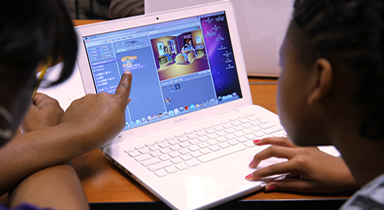
\includegraphics[width=1\linewidth]{assets/similar-games/scratch.jpg}
    \caption{Scratch~\cite{a2022_scratch}}
    \label{fig:scratch}
\end{figure}

Scratch is one of the~most extensive coding applications with a~simple visual interface that allows the~creation of universal programs, as can be seen in the~figure~\ref{fig:scratch}.

After entering the~game, a~user sees several projects of other users, which they can open and try.
If the~user opens a~game, they see a~game window, instructions for playing, and other notes and credits.
If the~user is interested in how the~game is programmed, they can see the~inside, which takes them to its editor screen.
They can then create a~remix for the~game, an~open continuation of the~original game with any modifications.

It is already clear from the~mentioned progress that the~game Scratch is \mbox{focused} on open creation and encourages the~creativity of its players.
\linebreak
The~user can create a~new game.
The~only means are the~editor's free area and the~blocks on the~window side that can be moved and combined to achieve the~desired effect~--- to program the~game according to the~user's idea.

The~editor provides a~wide range of visual commands divided into several categories.
There are categories like motion, looks, sound, events, etc.
Each such category contains several visual commands that interact with the~game character or the~world differently.
These commands consist of individual blocks glued together in the~editor area.
All commands under the~current command are stuck to it, and if the~user grabs a~command, anything stuck under it will be grabbed with it.
Commands are placed anywhere in the~area, and there is no fixed grid.

\pagebreak
Players can create games, animation, and other visual creations.
That promotes problem-solving skills and collaboration.
According to~\cite{a2022_scratch}, Scratch is a~nonprofit organization, widely available in more than 70 languages, and designed for ages 8 to 16.
The~game is also completely free.

Although Scratch has no story, it does contain a~few more miniature tutorials that bring the~user closer to the~editor and its abilities.
Since the~game does not have fixed rules for the~games created, the~created games have no score for fulfillment.
The~only measure can be the~number of impressions, likes in the~form of stars and hearts, and the~number of remixes created. 

\section{Khan Academy}
\label{similar-games:khan-academy}

\begin{figure}
    \centering
    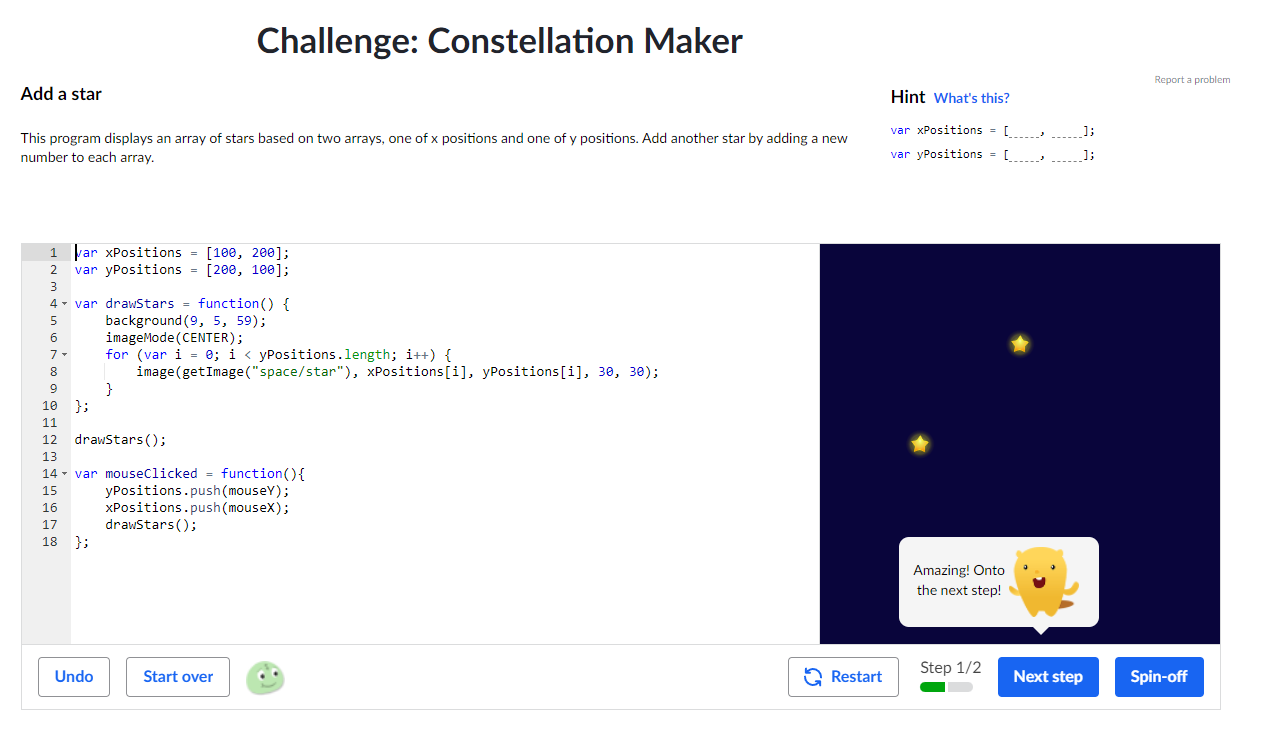
\includegraphics[width=1\linewidth]{assets/similar-games/khanacademy.png}
    \caption{Khan Academy~\cite{a2022_khan}}
    \label{fig:khanacademy}
\end{figure}

Khan Academy is one of the~most extensive generic purpose educational\linebreak{}applications with gamification elements.
\textcquote{a2022_khan}{For every student, every classroom. Real results.}
They provide interactive learning materials for math, science, history, economics, etc.
It includes instructional videos supplemented by interactive quizzes and study materials.

After entering the~website, users see all the~Khan Academy's courses.
There are a~vast number of them, and the~courses themselves contain even more individual tasks.
One of the~main focus of the~courses is the~teaching of mathematics, which covers content from primary school, through secondary school, to some topics of university mathematics.

\pagebreak
When clicking on one of the~math courses, the~user is shown a~screen with many units.
On the~side of the~screen, there is also a~summary of the~given units.
That visually represents the~status of the~given parts.
Each unit has several tasks that are either educational, for example, in the~form of text or, more often, video, and several practice tasks that verify the~knowledge gained from the~unit.
The~practice tasks themselves are created visually, and therefore, for example, not only the~example \mintinline{text}|2+3=?| is displayed.
Most of the~time, there is also a~visual representation like two blue boxes and three red ones or marking the~sum on the~axis, etc., according to the~settings of the~given task.

The~application contains the~Computer programming course, which covers an~intro to JS, HTML, CSS, and SQL languages.
The~College Computer Science Principles course covers digital information, the~Internet, cybersecurity, programming, algorithms, simulations, and data analysis.
These courses draw on canvas in JavaScript or do websites using HTML and CSS.

Programming tasks often take the~form of challenges, where the~user\linebreak{}receives a~text entry, a~small help, and an~editor in which they can write the~solution of the~task.
An example of a~challenge can be seen in the\linebreak{}figure~\ref{fig:khanacademy}.
Such a~challenging task can also have several steps, and the~task automatically recognizes the~completion of the~current part.
After completing the~task, the~user will have a~button to create a~spin-off if they want to improve the~task and engage in the~solution with their creative spirit.

It also provides a~feature to create and manage classes.
Therefore, teachers can create a~class and invite their students to join.
Then, teachers can create assignments and see students' performances, scores, etc.

According to~\cite{a2022_khan}, Khan Academy is available in more than 50 languages and is free to use.
They are partnered with several schools in the~United States.
And they have more than 130 million registered users in more than 190 countries.
For kids aged 2 to 8, there is also a~learning game-like application called Khan Academy Kids that provides a~joyful and engaging learning curriculum for young children.

\section{CodeCombat}
\label{similar-games:code-combat}

\begin{figure}
    \centering
    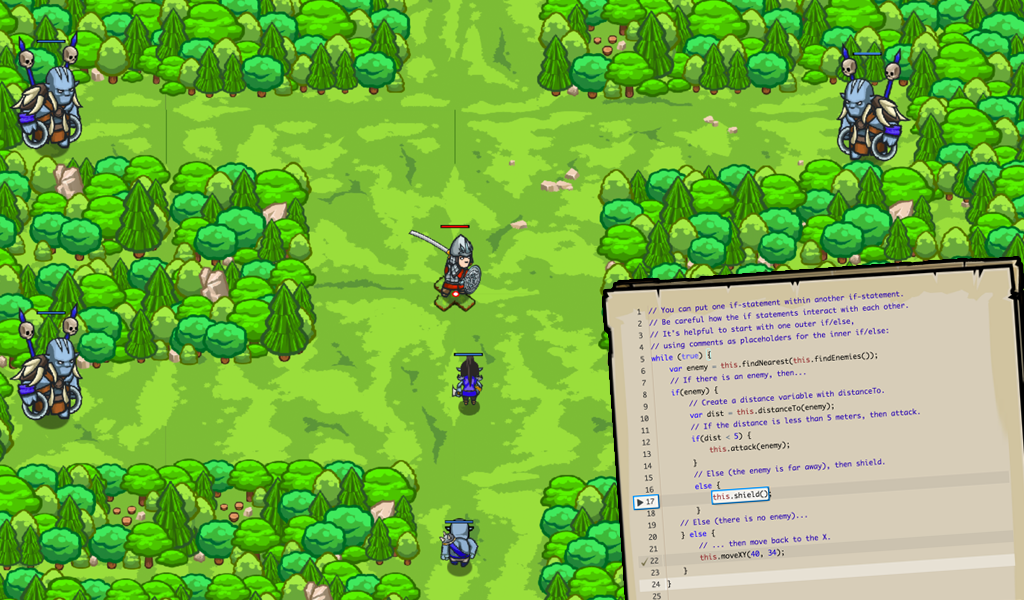
\includegraphics[width=1\linewidth]{assets/similar-games/codecombat.png}
    \caption{CodeCombat~\cite{a2022_codecombat}}
    \label{fig:codecombat}
\end{figure}

CodeCombat is one of the~representatives of a~very story-driven game in which the~player controls a~character through programming.
It is a~community project where volunteers create levels and add features.
Players have their characters with stats and items that add new features to the~player in a~game.

As CodeCombat mentions~\cite{a2022_codecombat}, \textquote{Programming is magic.}
They provide wizard-like features to players so they can use their pure imagination to solve game missions.
And according to the~game, this approach enables players to learn faster.

After entering a~game, the~player sees several game maps.
However, the~player often has to finish the~previous ones to make them available.
The~novice player has the~first game map at their disposal, which guides the~player through the~basic concepts of programming and controlling\linebreak{}the~game itself.
Each map includes a~path that intersects the~points that contain game missions.
The~player must pass these points gradually.
The~whole game is styled in a~medieval RPG style, as can be seen in the~figure~\ref{fig:codecombat}.

After starting the~game mission, the~player sees the~playing area and the~goals they must meet.
In addition, the~window may also display smaller help.
In the~corner of the~game, the~goals are displayed, which are marked if the~player has met them.
After completing the~mission, a~dialog box will appear where the~player will be credited with experience points.

The~player can choose one of several languages for programming: Python, JavaScript, CoffeeScript, and Lua.
Languages C++ and Java are available for subscribers.
The~player can play as one of several avatars, each with different abilities and skills.
Some are warriors, others are archers, and others are mages.

Optional missions are also shown on the~map, but they are only accessible to subscribers.
The~player can get a~more extensive selection of avatars and access to more than 500 missions for a~subscription.

\pagebreak
\section{Minecraft}
\label{similar-games:minecraft}

\begin{figure}
    \centering
    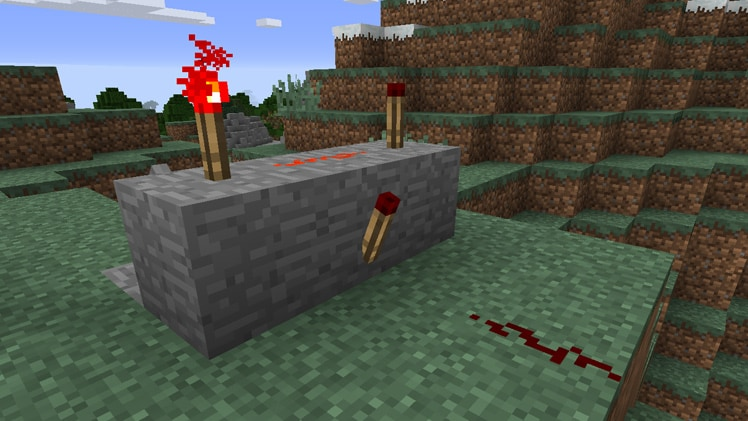
\includegraphics[width=1\linewidth]{assets/similar-games/minecraft.jpg}
    \caption{Minecraft~\cite{a2022_minecraft}}
    \label{fig:minecraft}
\end{figure}

Minecraft is the~most famous building game.
Its minimalistic graphics, where all worlds are made of cube blocks, support creative thinking and creating experiences~\cite{a2022_minecraft}.
It also has an~Education Edition, which focuses on generic purpose education.
That means people can play or create different educational content in the~Minecraft world for any subject.
Both Minecraft: Education\linebreak{}Edition and Minecraft have ways of introducing programming to children.
\linebreak
Minecraft costs about €24, and anyone can play Education Edition with\linebreak{}a~Microsoft 365 account.

Minecraft is mainly a~building game.
However, builders also want to build interactive buildings or automate things, so there is Redstone powder in the~game, as can be seen in the~figure~\ref{fig:minecraft}.
That is an~entity that can be placed on blocks and is used to transmit a~signal.
The~game also provides several blocks and entities that can work with the~signal.
These can be, for example, basic buttons and sensors, but also an~archery target, a~light sensor, a~music block, and more.

Some blocks can transmit a~redstone signal, others can receive, and some can do both.
The~restone signal gradually loses its power over the~distance travelled.
The~signal loses all power when more than 15 blocks from the~source.
The~game also includes a~redstone repeater and comparator to manipulate the~redstone signal.
A repeater is a~block used to repeat the~total signal strength and can also delay the~signal or determine the~direction of the~signal.
A comparator is a~block that can compare or subtract signals.

\pagebreak
Other special blocks are, for example, a~piston that can move blocks.
These and other special blocks give players of this game quite versatile programming skills.
The~only downside may be that the~blocks have to be physically placed, and the~design of such a~redstone circuit can be very complicated.

Minecraft: Education Edition is a~version of Minecraft designed for schools and education.
It is no longer primarily intended for open-world exploration but more for exploring created learning missions or creating worlds through programming.

The~Code Builder tool is used for programming, in which the~player can program an~agent that executes commands for them.
The~agent is programmed either in JavaScript or using Scratch-style visual programming.
The~agent can do every type of action an~ordinary player would be able to do.

Another option in Minecraft: Education Edition is the~Chemistry Lab, where players can get acquainted with the~elements and their creation,\linebreak{}compounds, etc.
With this feature, players can learn chemistry and have interactive school lessons.

Minecraft is very popular due to the~modding.
That means players can develop unique modes to customize the~world and game mechanics.
For example, developers can create a mod that adds Pokemons to expand the~Minecraft world.

\begin{figure}
    \centering
    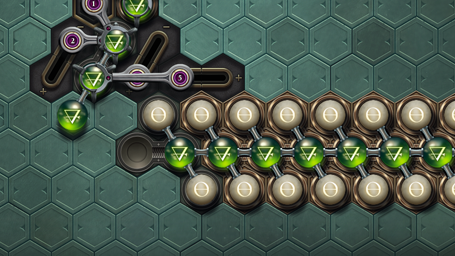
\includegraphics[width=1\linewidth]{assets/similar-games/opusmagnum.png}
    \caption{Opus Magnum~\cite{a2022_zachtronics}}
    \label{fig:opusmagnum}
\end{figure}

\pagebreak
\section{Opus Magnum}
\label{similar-games:opus-magnum}

Opus Magnum is an~exciting game that takes place in an~alchemical world.
\linebreak
According to~\cite{a2022_zachtronics}, the~player's goal is to assemble potions, move them,\linebreak{}transmute them, etc., to complete open-ended puzzles.
The~game contains a~transmutation engine.
This engine allows players to place machines that operate according to a~program.
An example of the~game can be seen in the~figure~\ref{fig:opusmagnum}.

In each mission, the~player must produce a~specific alchemical product.
They achieve this using the~transmutation engine.
The~player places elements and components in the~game and uses them to try to produce the~targeted product.
The~game is divided into hexes, and arms are used to move the~elements.
Arms can rotate and move elements closer or further.
There are several types of arms, some of which can handle only one element, some of which can hold more than one element at a~time.
There are also tracks in the~game that can transport elements by rail.
And glyphs that can join elements together or transform into another element.

These mechanical parts are controlled by programming.
At the~bottom of the~game is a~panel with programmable sequences.
According to the~sequences, mechanical parts are controlled.
Players can also compete with each other in three criteria.
One is the~total price, where each mechanical part costs a~certain amount of money.
The~second is the~area of the~table that the~player's machine took.
And the~third is the~number of actions that the~player's machine has performed.
The~game shows histograms and individual statistics among friends on Steam (a game distribution service) for these three criteria.
Players are challenged to make their engines smaller and faster and embrace symmetry and infinity.
The~game also contains a~solitaire minigame.

The~game's background contains a~sophisticated story with other alche\-mists and the~city's ancient Houses, where the~game missions occur.
The~story also introduces the~basic concepts necessary to understand the~game.
\linebreak
The~graphics are situated in the~dark world of alchemists.
Although the\linebreak{}graphics are excellent, novices or children could have problems with the~game's programming mechanics in the~beginning.
A good element is providing\linebreak{}feedback on cost, cycles, and area statistics in which friends can compete.
The~game is not free; it costs around €16.

The~game, according to~\cite{a2022_zachtronics}, provides a~puzzle editor.
Players can use it to create their game missions.
These can then be saved to the~Steam Workshop, and other players and their friends can play the~player's mission.

\pagebreak
\section{7 Billion Humans}
\label{similar-games:7-billion-humans}

\begin{figure}
    \centering
    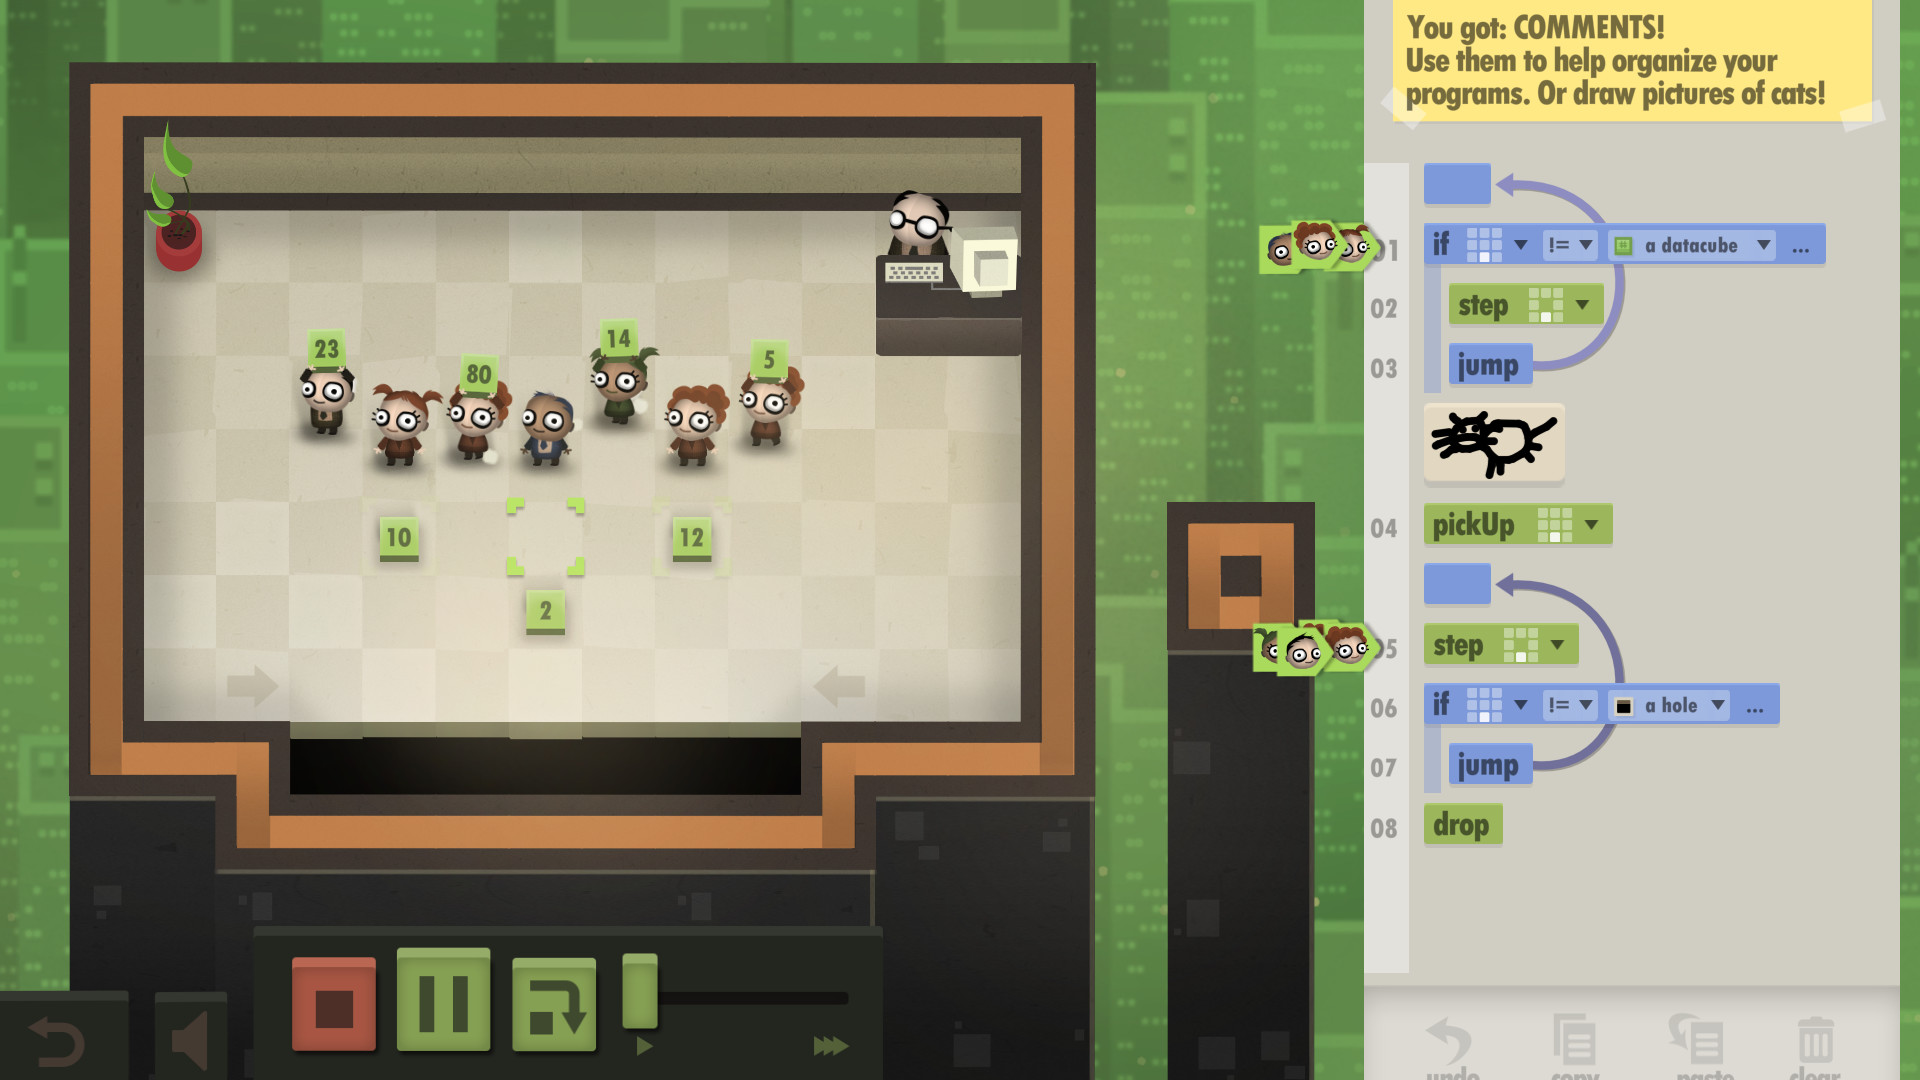
\includegraphics[width=1\linewidth]{assets/similar-games/7bilionhumans.jpg}
    \caption{7 Billion Humans~\cite{a2022_tomorrow}}
    \label{fig:7bilionhumans}
\end{figure}

7 Billion Humans is a~puzzle game where your task is to program a~parallel computer made of people, as can be seen in the~figure~\ref{fig:7bilionhumans}.
\mbox{Therefore}, the~player's job is to figure out how to synchronize workers to achieve\linebreak{}the~expected outcome.

The~players are presented with simple, stylish graphics.
Players have to solve programming puzzles, and each game mission has a~specific task.
They have human workers who follow the~visual commands.
Data cubes are often used in tasks.

Interestingly, the~same program is used to program all human staff at once.
Of course, each employee works with the~program individually according to their surroundings and internal logic.
That requires players to engage in wit in creating such a~sequence of commands to make the~game come true.

According to~\cite{a2022_tomorrow}, once the~player comes up with a~working solution,\linebreak{}the~game performs another 25 cases in which they randomly exchange data like in the~data cubes, thus testing the~quality of the~solution.
Optional game tasks are overcoming the~average number of steps and average time.
This concept motivates players to optimize programs.

The~biggest drawback for inexperienced players might be that the~game does not explain the~concepts.
But the~concepts are simple so that players can get into it quickly.
The~game costs around €12.

\section{Codewars}

\begin{figure}
    \centering
    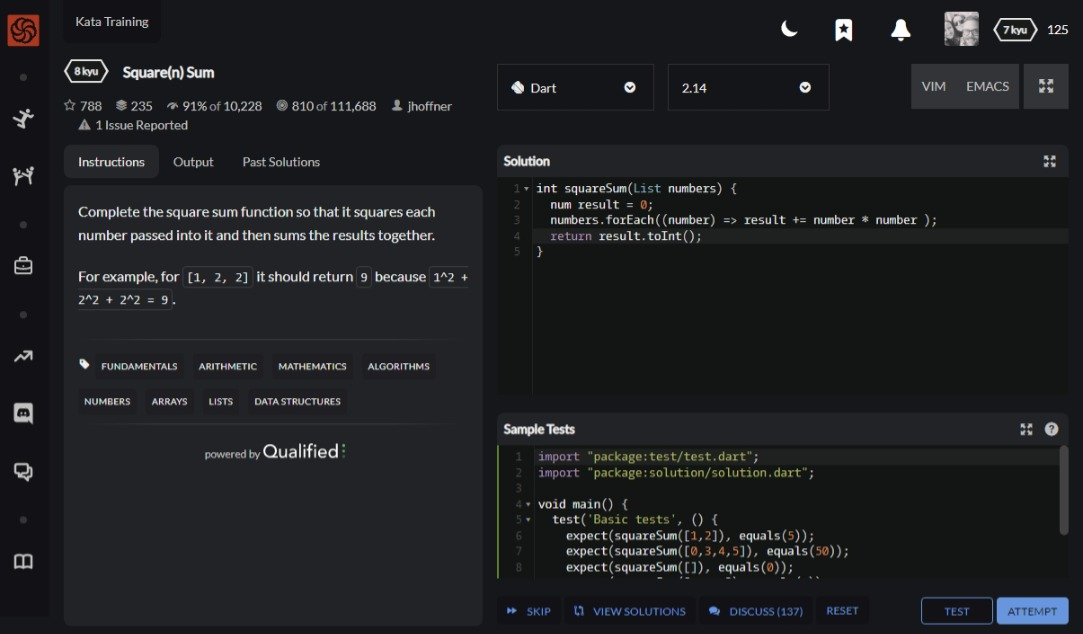
\includegraphics[width=1\linewidth]{assets/similar-games/codewars.jpeg}
    \caption{Codewars~\cite{a2022_codewars}}
    \label{fig:codewars}
\end{figure}

Codewars is a~game that provides a~place for independent tasks.
The~game has no story or fixed order of tasks.
Instead, the~tasks have tags that distinguish their focus, and the~player themselves chooses the~engaging exercises they want to play.
That makes this game very unique.

These tasks, which are code challenges, are called \textquote*{kata}.
Each kata has a~Kyu/Dan rank, indicating its difficulty.
According to~\cite{a2022_codewars}, these terms are borrowed from Japanese martial arts.
The~master level is called Dan, and Kyu indicates the~number of levels from that level.
Beginners thus have 8~kyu.
Conversely, the~best grade is 4~dan.
Each player has a~Kyu/Dan rating, and the~player progresses when they complete the~kata of the~same or higher level.

In addition, the~game has an~honor system, which is obtained by creating a~kata, constructive commentary, and promising solutions.
This system is therefore based on community evaluation.
Together, these concepts form a~fascinating combination in teaching, similar to martial arts.

The~player can use over 20 programming languages such as Python,\linebreak{}JavaScript, etc.
Each kata has its description and instructions, where\linebreak{}the~player learns what the~task is focused on.
Players also see sample tests that the~generated code must pass.
Then the~players try to write a~code that will meet the~requirements.
If players do not know how to complete a~kata, they can unlock a~reference solution, but that will deprive them of the~\mbox{opportunity} to gain a~kata rank or honor.
They can also open a~discussion to ask about problems or other advice.
A sample of the~kata screen can be seen in the~figure~\ref{fig:codewars}.

\pagebreak
Katas are met by passing tests.
If the~player programs a~solution, they can test it against the~sample input.
These usually cover units of simple cases.
Once these tests are completed, the~code can be tested on a~larger sample of tests and then submitted.

Codewars is suitable for getting out of players' comfort zone.
Individual katas are challenging, cover a~variety of cases, and allow players to try new things and approaches.
Players can also learn a~new programming language that they can try out in practice and even create solutions in multiple languages.
Some katas require geometry and algebra, which players will also repeat.
And one of the~most beneficial uses is the~opportunity to learn from the~solutions of others.
And of course, compete and compare with friends. 

\section{CodeMonkey}

\begin{figure}
    \centering
    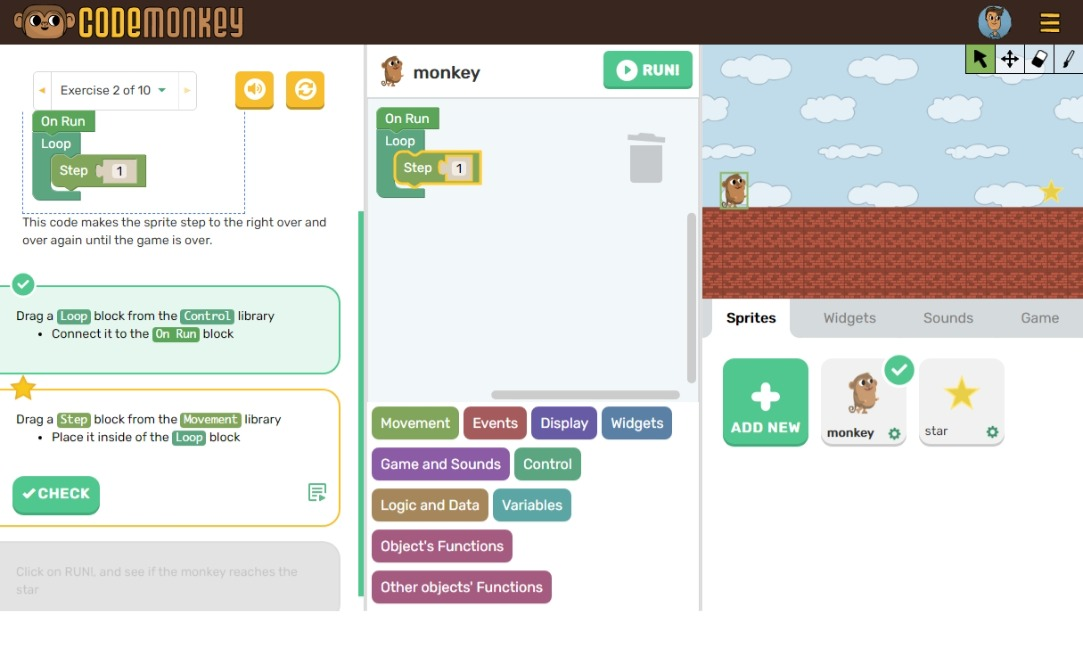
\includegraphics[width=1\linewidth]{assets/similar-games/codemonkey.jpeg}
    \caption{CodeMonkey~\cite{a2020_codemonkey}}
    \label{fig:codemonkey}
\end{figure}

CodeMonkey is a~game focused on teaching programming to children.
\linebreak
The~game contains several separate courses, each with a~different story and a~different form of programming.
Simplified visual programming with \mbox{picture} boxes is available for the~youngest children and beginners.
Other courses then use visual programming blocks similar to Scratch.
And other more \mbox{advanced} courses use text programming using Python or CoffeeScript.
The~game\linebreak{}provides students with various educational resources that provide learning material for the~youngest to the~oldest.

\pagebreak
According to~\cite{a2020_codemonkey}, CodeMonkey provides classroom support for schools in which students can be managed.
The~teacher sees the~statistics, can assign tasks and can set up an~automatic evaluation.
The~game is used by over 25 million students and over 120,000 teachers.
Of course, the~game can be played as an~individual outside of school, from home comfort.
The~game also supports web and mobile applications, making it accessible to most players.

After logging in to the~game, the~user sees many available courses.
Each is marked for novices, beginners, intermediate or advanced.
It also indicates which method is used for programming: block coding, text coding, etc.
Players will see a~slightly different game window based on the~method used.
Usually, however, the~player has a~command panel, whether in visual or textual form, and a~game panel.
The~assignment is displayed to the~player in the~panel itself or is gradually communicated using dialog boxes.
Game missions with block coding in a~version similar to Scratch also have progressive goals that are marked if the~user accomplishes them.
Each goal also has advice on how to meet them.
The~player can use various sprites, widgets, sounds, and command blocks in this Scratch-like environment.
An example of the~game mission can be seen in the~figure~\ref{fig:codemonkey}.

As in Scratch, players can create their games using text or visual programming.
However, the~game builder editor is only available to subscribers.
Players can see the~creations of others, which they can also try, evaluate and remix.

The~game includes ten free courses but includes an~additional twenty-one for subscribed players.
The~cheapest individual license costs about \$6 per month.
Unique school plans are available for schools, which must be agreed upon individually.

\section{Codemancer}

\begin{figure}
    \centering
    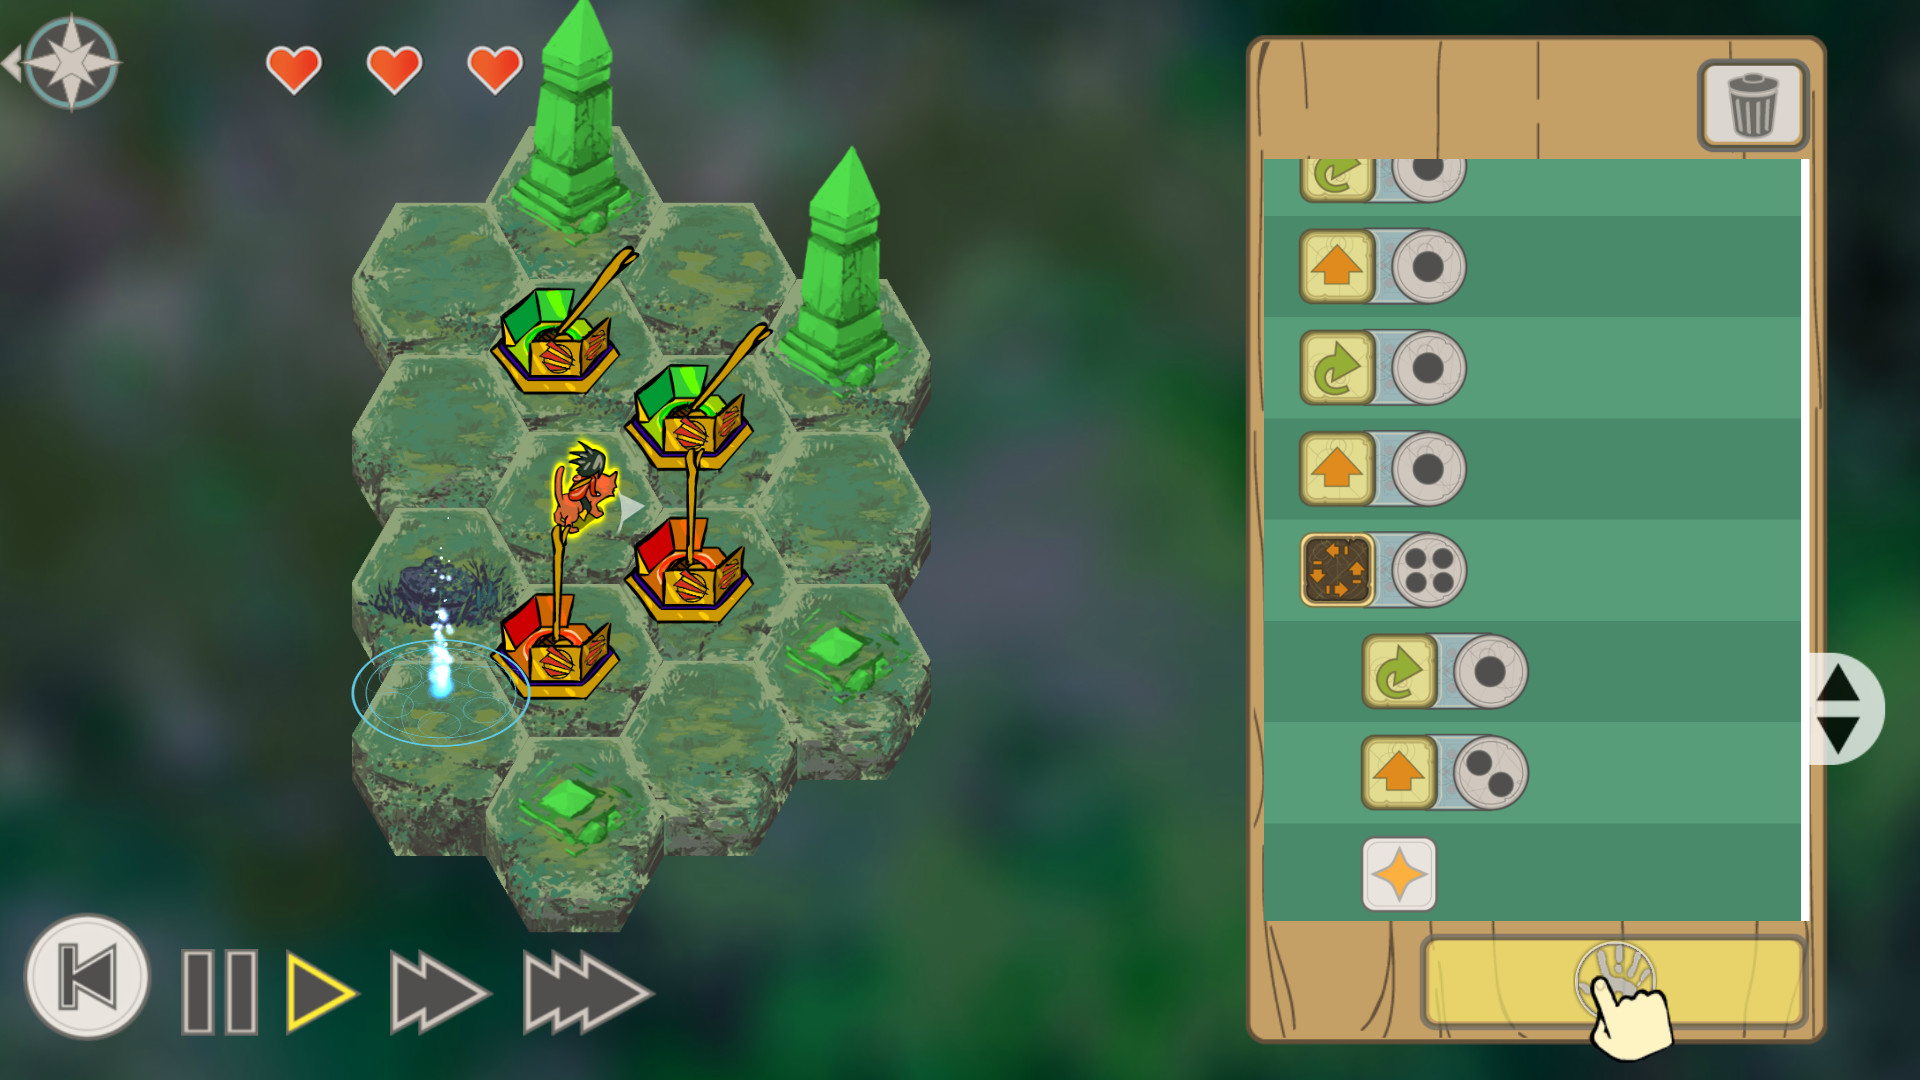
\includegraphics[width=1\linewidth]{assets/similar-games/codemancer.jpg}
    \caption{Codemancer~\cite{a2021_codemancer}}
    \label{fig:codemancer}
\end{figure}

Codemancer is an~educational game that teaches programming to children.
\textcquote{a2021_codemancer}{A fantasy game that teaches the~magic of code,} as stated by their site.
According to~\cite{a2021_codemancer}, the~game is aimed at children aged 6 to 12.
It has a~moving fantasy story that is a~big part of the~game.
The~story revolves around a~little girl Aurora, who is trying to grow up and is facing obstacles.
The~girl must learn the~magic which she must use to save her father.

In the~game, players use commands in the~form of special runs.
These runes can be modified in an~attached box, where the~player can usually \mbox{select} the~number of repetitions.
Typically, the~player selects a~rune to move and modifies its number so that, for example, the~character moves three times.
Similarly, it can modify the~rotation rune.
The~game takes place on\linebreak{}a~hexagonal grid, on which is the~player's character, the~girl Aurora, whom the~player controls, as can be seen in the~figure~\ref{fig:codemancer}.

An exciting concept is how the~steps are performed.
The~player does not have to set all the~steps immediately but can perform graduate sequences one after the~other.
The~character can rotate one hex to the~right and take two steps forward, and in the~following sequence, they can turn left and take action.
That adds an~exciting aspect of gradual development to the~game.
As the~game progresses, the~game shows players new programming concepts such as cycles, variables, conditions, and functions. 

The~game is available on mobile devices and desktops.
It is available for free at the~Steam store, which distributes the~game for desktops, and the~App Store distributes the~game on Apple devices.
It is available for about €5 in the~Google Play store, which distributes the~game on Android.

\section{Baba Is You}

\begin{figure}
    \centering
    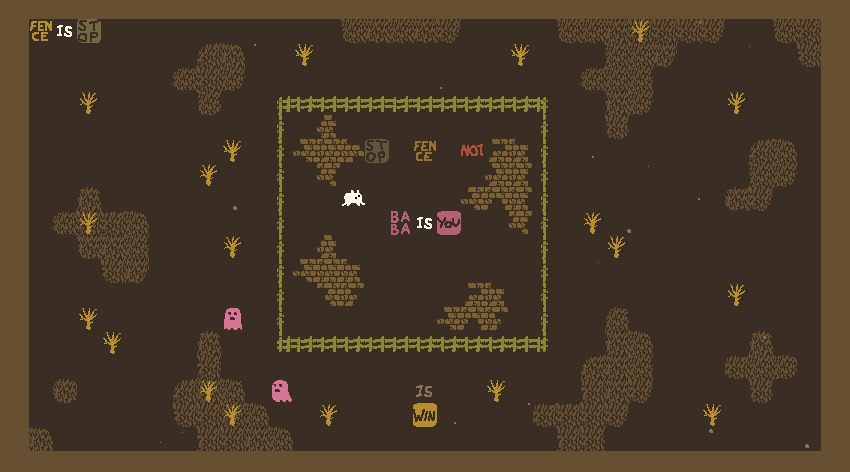
\includegraphics[width=1\linewidth]{assets/similar-games/baba.png}
    \caption{Baba Is You~\cite{a2022_baba}}
    \label{fig:babaisyou}
\end{figure}

Baba Is You is a~very different game.
While in previous games, players \mbox{create} sequences using blocks or by writing code, in this game, the~game itself programs the~game.
The~game character can move blocks that are composed of text.
These text blocks can create another combination, such as allowing a~character to walk through a~wall or change a~character to another object, even to a~wall.

According to~\cite{a2022_baba}, the~game relies on manipulating the~rules that are part of the~game, and the~player's goal is to change and abuse these rules to their advantage.
The~game has simple pixel graphics that add a~pleasant atmosphere, as can be seen in the~\ref {fig:babaisyou}.
The~mechanics themselves, where the~rules are incorporated into the~game itself, and the~game is governed by changing rules, is an~exciting way for one to improve in problem-solving.

The~object of the~game may be, for example, to touch a~flag that signifies victory in a~given mission; if the~rules of the~game mention it.
But the~problem is how to get to the~flag.
In addition, the~game map consists of several walls, rooms, and other blocks that the~character cannot pass.
Touching some blocks can mean a~defeat.
The~player's goal is to find such game rules and modifications so that the~player reprograms the~game and wins the~mission.

The~game is available on Windows, Linux, and macOS desktops for around \$15.
The~game contains over 200 levels that players can play.

\section{Evaluation}

All the~mentioned games have fascinating concepts and mechanics, thanks to which players, and therefore children, can improve their programming skills.
However, none are available for free (without significant restrictions),\linebreak{}contain an~exciting and engaging story, and provide study materials at the same time.
Therefore a~game with gamification features mentioned in chapter~\ref{analysis} will be designed and implemented.

Each game has unique features by which the~proposed game can be\linebreak{}inspired.
Scratch has tools for creative game development using visual programming and promotes healthy competitiveness, but it is not very focused on teaching and story.
Khan Academy has an~extensive curriculum and many challenges, but it is not focused on the~story.
CodeCombat has an~exciting story and, with the~help of excellent graphics, allows children to learn to program, but the~free version can be limited in time.
Minecraft has a~uniquely integrated programming feature to the~in-game world, but it focuses\linebreak{}on exploring and creating worlds rather than on teaching and the~story\linebreak{}itself.
Opus Magnum has joyful visual programming tools with an~engaging, mysterious story in the~background, but not available for free.
7~\mbox{Billion} \mbox{Humans} is an~exciting game with nice graphics and parallel programming, but it lacks a~deeper story and teaching materials.
CodeWars is more suitable for self-study with challenges than teaching with a~plan.
\mbox{CodeMonkey} contains a~wide variety of programming missions and various programming approaches, but the~options of the~free version are limited.
Codemancer is partially free and provides an~exciting story around which the~whole game revolves, but more complex concepts are not much explained, and the~game is more suitable for more minor children.
And Baba Is You is a~great-looking and exciting game, but it is more suitable for practicing problem-solving than\linebreak{}teaching programming.

The~designed game should incorporate all these games' benefits into itself.
The~game should have good storytelling, create a~joyful visual programming tool that can be easily understood by children, and provide a~way how players can learn basic and advanced concepts. 
The~proposed game should also be accessible and open-source to provide its content to students for free while making the~code available to other developers who may be looking\linebreak{}for inspiration.

Criteria for comparing similar games are shown in the~table~\ref{table:similargames}.
\linebreak
As mentioned, the criteria are comprehensibility~(\mintinline{text}{CO}), story~(\mintinline{text}{ST}), study\linebreak{}materials~(\mintinline{text}{SM}), feedback~(\mintinline{text}{FB}), and whether the game is free of charge~(\mintinline{text}{FC}).

\begin{table}[b]
    \catcode`\-=12
    \centering
    \begin{tabular}{lccccc}
    \toprule
     & \multicolumn{5}{c}{Criteria} \\
    \cmidrule(l){2-6} 
    \multicolumn{1}{l}{Game} &
        \multicolumn{1}{c}{CO} &
        \multicolumn{1}{c}{ST} &
        \multicolumn{1}{c}{SM} &
        \multicolumn{1}{c}{FB} &
        \multicolumn{1}{c}{FC} \\
    \midrule
                         Scratch                       & $\ast$ &        &        &        & $\ast$ \\
    \rowcolor[gray]{.95} Khan Academy                  &        &        & $\ast$ & $\ast$ & $\ast$ \\
                         Code Combat                   & $\ast$ & $\ast$ & $\ast$ & $\ast$ &        \\
    \rowcolor[gray]{.95} Minecraft                     & $\ast$ &        &        &        &        \\
                         Minecraft: Education Edition   & $\ast$ &        & $\ast$ & $\ast$ & $\ast$ \\
    \rowcolor[gray]{.95} Opus Magnum                   &        & $\ast$ & $\ast$ & $\ast$ &        \\
                         7 Billion Humans              & $\ast$ &        &        & $\ast$ &        \\
    \rowcolor[gray]{.95} Codewars                      &        &        &        & $\ast$ & $\ast$ \\
                         CodeMonkey                    & $\ast$ & $\ast$ & $\ast$ & $\ast$ &        \\
    \rowcolor[gray]{.95} Codemancer                    & $\ast$ & $\ast$ & $\ast$ &        & $\ast$ \\
                         Baba Is You                   & $\ast$ &        &        &        &        \\
    \bottomrule
    \end{tabular}
    \caption{Comparison of Similar Games}
    \label{table:similargames}
\end{table}
\chapter{Design}
\label{chapter:design}

This chapter designs the~game's prototype according to the~analysis done in chapter~\ref{analysis}.
The~outputs of this chapter are use cases that uses described functional requirements, designed game mechanics, selection and a~description of the~architecture, a~discussion and design of a~client and server applications and database, and creation of user interface design.

\section{Use Cases}

A use case is a~term that describes how actors use a~program to achieve specific goals.
They describe and organize functional requirements from the~end users' point of view.
They are sequences of events and interactions that users can easily follow to achieve specific goals.
Use cases have primary and can optionally have secondary scenarios of their flow.

Each use case has a~name, triggering events, and the~main flow of events.
The~name contains a~verb and a~noun that express the~goal of the~use case.
The~triggering events describe an~initiation of the~use case.
Each use case can have multiple triggering events.
And the~main flow of events, step by step, describes the~flow of interactions between the~system and the~actor.
Optionally, use cases can also have preconditions.
Preconditions are conditions that must be met before executing the~use case.
Initiation and preconditions are a~part of the~flow, but they can be described separately.

Use cases of designed game recognize two actors: an~Anonymous User, an~actor who is not signed in to the~game, and a~Player, an~actor who is signed in to the~game.
The~Player is an~extension of the~Anonymous User.
That means that the~Player can use or execute everything the~Anonymous User can use or execute.

\let\oldsubsection=\thesubsection
\renewcommand\thesubsection{UC\arabic{subsection}}

\pagebreak
\subsection{Sign Up}

This use case describes signing up for the~game and is used by an~Anonymous User who, if processed successfully, becomes a~Player actor. If a~Player actor tries to activate the~use case, they are redirected to the~main screen.

This use case starts when an~actor navigates to the~sign-up screen or activates the~sign-up button.

\begin{enumerate}
    \item the~game navigates the~actor to the~sign-up screen.
    \item the~actor fills in their username, real name, email, password, and description into text inputs.
    \item the~game determines the~validity of the~actor's data.
    \begin{enumerate}
        \item If no issues were found, the~game signs in the~actor and navigates them to their profile screen.
        the~actor becomes a~Player.
        \item If issues were found, the~game announces the~fail.
    \end{enumerate}
\end{enumerate}

\subsection{Sign In}

This use case describes the~signing in the~game, and only an~Anonymous User can use it. If a~Player actor tries to activate the~use case, they are redirected to the~main screen.
If processed successfully, the~actor becomes a~Player actor.

This use case starts when an~actor navigates to the~sign-in screen or activates the~sign-in button.

\begin{enumerate}
    \item the~game navigates the~actor to the~sign-in screen.
    \item the~actor fills in their username and password into text inputs.
    \item the~game determines the~validity of provided username and the~corresponding password.
    \begin{enumerate}
        \item If no issues were found, the~game signs in the~actor and navigates them to their profile screen. the~actor becomes a~Player.
        \item If issues were found, the~game announces the~fail.
    \end{enumerate}
\end{enumerate}

\subsection{Sign Out}

This use case describes signing out of the~game, and only a~Player actor can use it.
After processing the~use case, the~actor becomes an~Anonymous User.

This use case starts when an~actor activates the~sign-out button.

\begin{enumerate}
    \item the~game signs the~actor out of the~game.
    \item the~actor is navigated to the~main screen.
\end{enumerate}

\subsection{View Publicly Available Game Information}

This use case describes viewing the~publicly available game information and other publicly available screens like the~main screen and about-us screen and its subscreens.
It can be used by an~Anonymous User actor, which also extends the~use to the~Player actor.

This use case starts when an~actor navigates to the~main screen, about-us screen, or its subscreens, activates the~main-screen button, or navigates to or activates any other screen or buttons, leading to screens with publicly available information.

\subsubsection*{Scenario a~-- Main Screen}

\begin{enumerate}
    \item the~game navigates the~actor to the~main screen.
    \item There, the~actor can view the~information.
\end{enumerate}

\subsubsection*{Scenario B -- About Us Screen}

\begin{enumerate}
    \item the~game navigates the~actor to the~about us screen (or one of its corresponding subscreens).
    \item There, the~actor can view the~information.
\end{enumerate}

\subsection{View Own Profile}

This use case describes viewing an~actor's in-game profile.
A Player actor can only use it.
If an~actor, not a~Player, tries to activate the~use case, they are redirected to the~sign-in screen.

This use case starts when an~actor navigates to the~profile screen or activates the~profile button.

\begin{enumerate}
    \item the~game navigates them to their profile screen.
    \item There, the~actor can view the~profile.
\end{enumerate}

\subsection{View Own Statistics}

This use case describes viewing an~actor's in-game statistics.
A Player actor can only use it.
If an~actor, not a~Player, tries to activate the~use case, they are redirected to the~sign-in screen.

This use case starts when an~actor navigates to the~statistics screen or activates the~profile button.

\begin{enumerate}
    \item the~game navigates the~user to their statistics screen.
    \item There, the~actor can view the~statistics.
\end{enumerate}

\pagebreak
\subsection{View Courses}

This use case describes viewing a~list of game courses~-- called stories~--, a~specific story, and a~list of the~story's missions.
A Player actor can only use it.
If an~actor, not a~Player, tries to activate the~use case, they are redirected to the~sign-in screen.

This use case starts differently based on its scenarios.

\subsubsection*{Scenario a~-- View Courses}

This scenario starts when an~actor navigates to the~stories screen or activates the~stories button.

\begin{enumerate}
    \item the~game navigates the~actor to the~stories screen.
    \item the~actor can view a~list of courses.
\end{enumerate}

\subsubsection*{Scenario B -- View Course}

This scenario starts when an~actor navigates to the~story screen or activates the~specific story button.

\begin{enumerate}
    \item the~game navigates the~actor to the~selected story screen.
    \item the~actor can view a~list of the~story's missions and the~story's name and description.
\end{enumerate}

\subsubsection*{Scenario C -- View Mission}

This scenario starts when, on the~story screen, an~actor activates the~mission's item or button.

\begin{enumerate}
    \item the~game displays a~popup containing additional data about the~mission.
    It displays the~mission's name and description.
    \item If it is a~storytelling mission, a~\textquote{read} button is displayed.
    \item If it is a~learning mission, a~\textquote{learn} button is displayed.
    \item If it is a~game mission, a~\textquote{play} button is displayed.
    \item the~actor can activate the~displayed button to leave the~screen.
\end{enumerate}

\pagebreak
\subsection{Use Missions}

This use case describes using and viewing the~game mission.
A Player actor can only use it.
If an~actor, not a~Player, tries to activate the~use case, they are redirected to the~sign-in screen.

This use case starts when an~actor navigates to the~story's mission screen or activates the~mission's item or button on the~story screen.

\subsubsection*{Scenario a~-- Storytelling Mission}

This scenario starts when an~actor navigates to the~storytelling mission or activates the~storytelling mission's item or button on the~story screen.

\begin{enumerate}
    \item the~game navigates the~actor to the~storytelling mission screen.
    \item the~actor is presented with a~list of texts that can be shown step by step by clicking the~next button.
    \item the~back-to-story button is displayed after the~actor progresses through all the~texts.
    \item Using the~back-to-story button, the~actor can leave the~screen to the~mission's story screen.
\end{enumerate}

\subsubsection*{Scenario B -- Learning Mission}

This scenario starts when an~actor navigates to the~learning mission or activates the~learning mission's item or button on the~story screen.

\begin{enumerate}
    \item the~game navigates the~actor to the~learning mission screen.
    \item the~actor is presented with a~learning text.
    \item a~back-to-story button is displayed.
    \item Using the~back-to-story button, the~actor can leave the~screen to the~mission's story screen.
\end{enumerate}

\subsubsection*{Scenario C -- Game Mission}

This scenario starts when an~actor navigates to the~game mission or activates the~game mission's item or button on the~story screen.

\begin{enumerate}
    \item the~game navigates the~actor to the~game mission screen.
    \item the~actor is presented with a~game grid, command list view, and buttons.
    \item the~user can add or move commands, run or stop the~current game or save the~current game -- as described in custom use cases.
\end{enumerate}

\subsection{Save Current Game}

This use case describes the~saving of the~actor's current game.
A Player actor can only use it.

This use case starts when an~actor activates the~save button on the~game mission screen.
Being on the~game mission screen is a~precondition of this use case.

\begin{enumerate}
    \item the~game loads the~current progress of the~commands presented in the~command list view.
    \item the~game saves those data, together with completed, size, and speed attributes. 
\end{enumerate}

\subsection{Play Current Game}

This use case describes the~playing of the~actor's current game.
A Player actor can only use it.

This use case starts when an~actor activates the~play button on the~game mission screen.
Being on the~game mission screen is a~precondition of this use case.

\begin{enumerate}
    \item the~game locks the~command list view, so the~actor cannot interact with it. 
    \item the~game loads the~current progress of the~commands presented in the~command list view.
    \item the~game process these commands.
    \item the~game starts presenting a~step-by-step progression of the~game grid.
    the~procession of each step is signalized by an~arrow next to a~command block.
    \item After a~presentation is done, the~game shows a~dialog with optional size and speed challenge attributes.
    \begin{enumerate}
        \item If the~game resulted in a~success, a~success dialog is presented with a~corresponding status message.
        \item If the~game resulted in a~failure, a~failure dialog is presented with a~corresponding status message and related error message.
    \end{enumerate}
    \item the~game unlocks the~command list view.
    \item the~game saves the~current progression, as described in the~separate use case. 
\end{enumerate}

\subsection{Stop Current Game}

This use case describes the~stopping of the~actor's current game.
A Player actor can only use it.

This use case starts when an~actor activates the~stop button on the~game mission screen while the~game is in progress.
Being on the~game mission screen with a~game in progress is a~precondition of this use case.

\begin{enumerate}
    \item the~game stops the~progressing game.
    \item the~game unlocks the~command list view.
    \item the~game does not save the~progression and does not show the~success or failure dialog. 
\end{enumerate}

\let\thesubsection=\oldsubsection

\subsection{Requirements Implementation Overview}

\begin{table}[]
    \centering
    \begin{tabular}{|c||c|c|c|c|c|c|c|c|}
        \hline
         & F1 & F2 & F3 & F4 & F5 & F6 & F7 & F8  \\\hline\hline
    UC1  & x  &    &    &    &    &    &    &     \\\hline
    UC2  & x  &    &    &    &    &    &    &     \\\hline
    UC3  & x  &    &    &    &    &    &    &     \\\hline
    UC4  &    & x  &    &    &    &    &    &     \\\hline
    UC5  &    &    &    & x  &    &    &    &     \\\hline
    UC6  &    &    & x  &    &    &    &    &     \\\hline
    UC7  &    &    &    &    & x  & x  & x  & x   \\\hline
    UC8  &    &    &    &    &    & x  & x  & x   \\\hline
    UC9  &    &    &    &    &    &    &    & x   \\\hline
    UC10 &    &    &    &    &    &    &    & x   \\\hline
    UC11 &    &    &    &    &    &    &    & x   \\\hline
    \end{tabular}
    \caption{Implementation of Use Cases and Compliance with Requirements}
    \label{table:usecases-requirements}
\end{table}

Use cases organize functional requirements. 
An overview of the~implementation of use cases by functional requirements can be seen in table~\ref{table:usecases-requirements}.

Use cases distinguish two actors, an~Anonymous User and a~Player.
The~Player actor is an~extension of the~Anonymous User actor.
The~competence of both actors and relationships of individual use cases can be seen in the~figure of the~Use Case Diagram~\ref{fig:usecasediagram}.

\begin{figure}
    \centering
    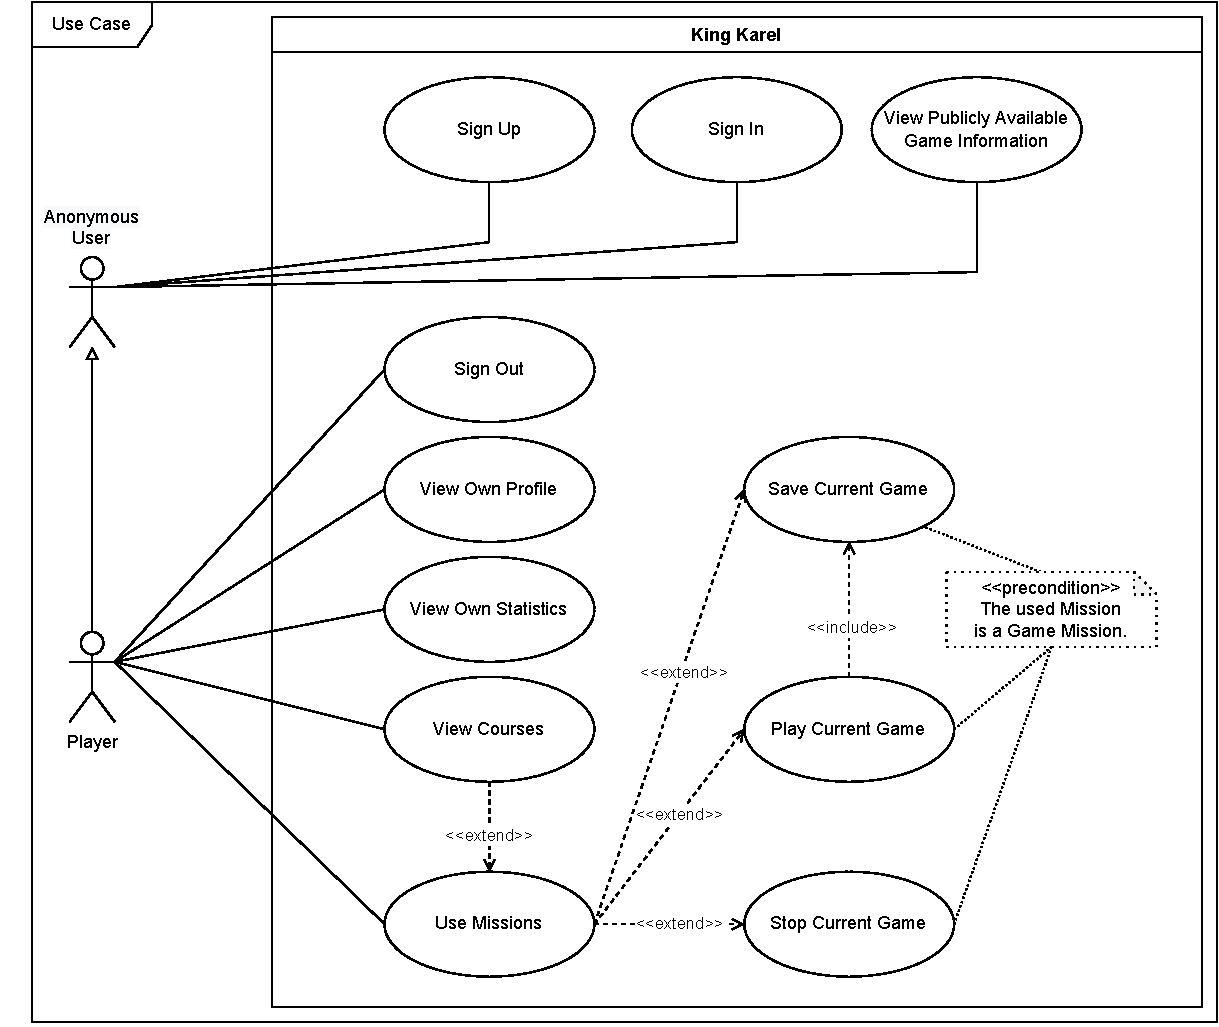
\includegraphics[width=1\linewidth]{assets/design/usecasediagram.pdf}
    \caption{Use Case Diagram}
    \label{fig:usecasediagram}
\end{figure}

\pagebreak
\section{Game Mechanics}

The~game's principle is to fulfill the~individual game missions with the~training courses gradually.
Because the~game is designed as an~educational game, users must first register.

The~game contains separate courses called stories.
The~story contains\linebreak{}several missions.
These can be of different types: storytelling, learning, and game.
The~goal is to gradually go through the~missions, read the~story in the~storytelling missions, and get used to it.
Storytelling missions have step-by-step messages to structure the~story.
In learning missions, the~goal is to learn information and new concepts and terms or improve on them.
\linebreak
The~information in these missions should be more comprehensive and may overlap.
Game missions are used to test the~acquired knowledge, understand the~task, come up with solutions, and overcome the~challenge.

The~very concept of the~game is based on the~fact that the~player uses command blocks to move the~playable character of the~robot Karel, the~king of the~game's story.
The~player tries to perform various tasks with him.
Command blocks are a~visual programming interface that needs to be inserted into the~command list in the~correct order and, if necessary, nested correctly.
However, there is no single correct solution.
In addition, the~command blocks must be valid, i.e., all their mandatory attributes must be set.
There are several types of command blocks.

Command \mintinline{text}|move <direction>| moves Karel one square in the~chosen\linebreak{}direction.
However, Karel can only move through the~boxes designated for this purpose.
For example, it must not hit a~wall, outside the~grid, water, etc.
If Karel manages to hit such a~square, the~game ends with an~error.

With the~\mintinline{text}|put mark| command Karel places one mark on the~square he is standing on.
However, there cannot be an~unlimited number of marks in a~square.
If Karel tries to put a~mark on a~square where there is no more space, the~game ends with an~error.

With the~\mintinline{text}|grab mark| command Karel takes the~mark from the~square he is standing on.
However, such a~mark must be on the~square.
If Karel tries to take the~mark from the~square where the~mark was not, the~game ends with an~error.

With the~\mintinline{text}|if <condition>| command Karel asks a~question.
The~question may be whether it can move in that direction one square.
It may also be up to the~marks whether Karel can remove a~mark from the~current square or place it on it.
Additional commands are nested in this command.
These will only be performed if the~business is evaluated successfully.
If the~condition is not evaluated successfully, the~command and the~nested commands are skipped.

The~\mintinline{text}|while <condition>| command works similarly to the~command\linebreak{}\mintinline{text}|if <condition>|.
The~difference is that Karel repeats the process as long as the~condition is met.
If the~condition fails the~first time, the~statement is not executed, and no nested statements are executed.

Using the~appropriate commands correctly makes it possible to compose a~tree structure of command blocks that solve the~given game mission.
\mbox{After} pressing the~play button, the~game evaluation starts.
The~evaluation is\linebreak{}stepped through, and the~player has the~opportunity to see which current command is being executed.
The~player also has the~opportunity to see where Karel is and which other squares are updated, i.e., where the~number of marks has changed.
The~player can stop the~game by pressing the~stop button. 

While passing through the~game, Karel collects optional size and speed attributes.
The~size attribute indicates the~number of blocks that were used.
The~speed attribute indicates how many times any block has been used.

The~final dialog will be displayed if an~error is encountered during the~evaluation or if the~game is evaluated successfully.
This dialog takes two forms, either successful or unsuccessful.
The~successful dialog displays a~success \mbox{message} and the~status of the~optional size and speed attributes.
These \mbox{attributes} have a~specified limit.
If a~player scores better than these limits, they receive a~bonus point for each attribute.
\section{Architecture}

A discussion and a~design on the~importance of good architecture must take place to comply with the~non-functional requirement of the~architecture.
\linebreak
A good software design is essential to keep the~software's code understandable, simple to extend, and easy to manage.
That applies to the~structure of all parts of the~software.
\textcquote{martin_2018_clean_architecture}{Software has two types of value: the~value of its behavior and the~value of its structure.
The~second of these is the~greater of the~two because it is this value that makes software soft.}
As mentioned in the~cited text, the~issue of software is not making its behavior correct and making it work as expected.
The~issues developers can face are caused by the~poor design of individual parts of the~software and its whole.
It's a~matter of quality, not quantity.

Many developers tend to write code fast.
They can even think that if the~code works, everything is fine.
That might be a~truth, but \textcquote{martin_2010_clean_code}{It is not enough for code to work.}
The~same functionality can be written in different ways and with various qualities.
No matter how the~code was written, it has to be flexible and easy to understand enough so developers can read it and refactor it easily.
Stated and all related reasons combined make software either good or terrible.

What caused developers to force themselves to write a~working software but with horrible designs?
Maybe companies that try to save money or release as fast as possible?
The~actual reason behind that does not matter.
Writing a~flexible, easily extendable, manageable, and easy-to-read code is not more complex than not doing that.
\textcquote{martin_2010_clean_code}{Indeed, the~ratio of time spent reading versus writing is well over 10 to 1.
We are constantly reading old code as part of the~effort to write new code. \dots{}
[Therefore,] making it easy to read makes it easier to write.}

The~code developers write really should be flexible to changes.
And the~same applies to the~design.
There is no reasoning behind not making it flexible.
Sticking to designing and coding too specifically might seem to work out at the~moment, but changes in the~future will be nearly impossible to make.
The~same also applies to extending features or adding new ones.
\textcquote{gamma_1994_design}{A design that doesn't take change into account risks major redesign in the~future.}
And many might argue that every code might be improved, and postponing writing flexible code instead of code that \textquote*{just works} is no big deal.
\textcquote{martin_2010_clean_code}{Of course bad code can be cleaned up.
But it's very expensive.}
Developers should instead use their time to design, build, and code, not to fix issues they could have avoided in the~first place.
\textcquote{martin_2018_clean_architecture}{The~only way to go fast, is to go well.}

Even if developers agree that individual parts of the~code should be written well, flexible, and easy to read and extend, why should they invest in making a~good design and architecture?
Because the~same issues that have been discussed in the~scope of individual parts of code also similarly apply to higher levels.
Choosing the~way of easy solutions now instead of proper design brings the~software into technical debt. 
\textcquote{martin_2018_clean_architecture}{Good architecture makes the~system easy to~understand, easy to~develop, easy to~maintain, and~easy to~deploy.
\linebreak
The~ultimate goal is to~minimize the~lifetime cost of~the~system
and~to~maximize programmer productivity.}

\subsection{Client-Server Architecture Design}

Multiple options should be considered to design the~best approach to create the~desired product.
There might be one program that handles everything, or multiple programs, that each does separate tasks.
The~software is often separated into the~server and client parts, no matter the~target platform.
Analyzed\linebreak{}requirements also require cross-platformness, as stated in non-functional\linebreak{}requirements.
Because of that, cross-platformness almost forces the~architecture to divide the~software into multiple parts.
The~software can be delivered as \mbox{individual} programs to each targeted platform.
Also, a~shared functionality can be extracted into a~separate part.
The~question is how many parts the~software should contain to offer the~best value and be the~easiest\linebreak{}to develop.

The~standard way of doing such software is to divide the~software into two parts: client and server.
A client part mainly handles the~aspect of displaying UI (user interface) to users.
Client application usually runs on the~user's device and relies on the~other part to perform or check some operations.
And a~server part that handles incoming requests and processes them.
The~server application also usually handles communication with a~database.
A database part can also be considered a~third part of the~software division.
For the~software to be cross-platform, the~software contains multiple client implementations, each for a~different targeted platform.
This way, the~software can have a~client for web, desktop, and mobile where all of these clients communicate with the~same server application.
That is very economical and also provides the~integrity of offered functionalities.

There are many ways in which client applications can be implemented.
According to~\cite{a2020_difference}, implementation strategies can also be divided into two types.
There are thick clients and thin clients.
Both of them provide benefits and disadvantages, and it is up to the~software designer to determine which type would fit the~current case the~most.
The~difference between them is which processes the~work, a~client or a~server?

Thin clients are designed to be small.
They usually process only the~data they have to, sending all extra data to a~server to process.
That might make thin clients easy to install, as they are usually smaller.
The~benefits of this approach might be that a~client application can be run almost anywhere, no matter the~hardware specifications, because the~thin client only\linebreak{}displays the~data, and the~actual processing and work happen in\linebreak{}a~server application~\cite{a2020_difference}.
The~disadvantages are that users often must rely on their internet connection, as most servers are in a~different network.

Thick clients are designed to be self-sufficient.
They usually use a~server application only as a~middleware that handles storing and fetching data from the~database.  
Thick clients handle and process most of the~data inside of the~client.
The~benefits of this approach are that even if the~client application loses an~internet connection or does not have one at all at the~moment, the~application can still do its work~\cite{a2020_difference}.
And the~data can be stored, synced, or verified later when the~internet connection is restored.
The~disadvantage that thick clients might face is that all versions of clients must implement all the~features that force developers to reinvent the~wheel.

Both thick and thin clients provide a~lot of benefits and disadvantages.
Therefore a~lot of the~time, some hybrid clients are used instead.
They combine those two approaches, making most of the~processing on the~server, especially if that is data-related, and making most of the~UI-related processing in the~client application.

The~designed game should implement a~hybrid-like type of client because it uses features of both approaches.
Its data must be stored in servers, but a~slow internet will suffice, yet it cannot work without it.
The~client part should process all UI-related functionality and game-related processing, but the~server should handle the~data storing, data processing and verifying, and authentication.

\subsection{Selection of Architectures for Client and Server}

As software development evolved and improved, new ways of designing and new architectures appeared and tried a~battle against time.
As mentioned in~\cite{a2021_clean_architecture_blog}, many architectures of systems try to achieve similar goals.
The~most common primary goal of architectures is to address the~separation of concerns.
Architectures like Hexagonal Architecture, Onion Architecture, and Clean \mbox{Architecture} separate concerns into different software layers.
Such architectures and their layers should be independent of UI, frameworks, databases, or other external tools.
If architecture depends on one of those things, it would significantly limit its abilities, which is not desirable.
Architecture should be generic and should not compromise with specific tools.

The~article~\cite{a2021_clean_architecture_blog} also mentiones the~dependency rule.
This rule describes requirements for a~flow of software layers.
Outer layers do specific things and use inner layers that describe policies.
Therefore, the~dependencies should always come from an~outer layer to an~inner layer.
Inner layers should not even know some outer layer exists.
This rule applies to all the~code inside the~layer, whether a~class, a~function, or any other entity.
The~inner layer commonly contains business rules like entities and use cases.
Outer layers commonly contain layers with interface adapters and frameworks.
The~number of layers can vary from architecture to architecture.
The~important thing is the~concept: the~separation of details and abstractions and that only details can point to abstractions, not the~other way around.
Architectures also must solve how to cross the~boundaries of layers and call abstractions that have to use details.
That is typically done by using the~dependency inversion principle described in~\ref{design:architecture:clean-archiecture}.

Both the~client and the~server parts should use a~good architecture that uses mentioned concepts.
The~goals are the~same: to create flexible and manageable codebases.
Both parts will use architectures similar to the~Clean Architecture, especially its dependency inversion principle and other SOLID principles.
\textcquote{martin_2018_clean_architecture}{Good software systems begin with clean code.
On~the~one hand, if the~bricks aren't well made, the~architecture of~the~building doesn't matter much.
On~the~other hand, you can make a~substantial mess with well-made bricks.
This is where the~SOLID principles come in.}

\subsection{The~Clean Architecture}
\label{design:architecture:clean-archiecture}

The~Clean Architecture was described in an~eponymous book~\cite{martin_2018_clean_architecture} authored by Robert~C. Martin, also known by the~nickname Uncle Bob.
The~author is an~American software engineer known for the~invention or promotion of~software principles, especially the~SOLID principles.
The~architecture can be seen in the~figure~\ref{fig:thecleanarchitecture}. 

\begin{figure}
    \centering
    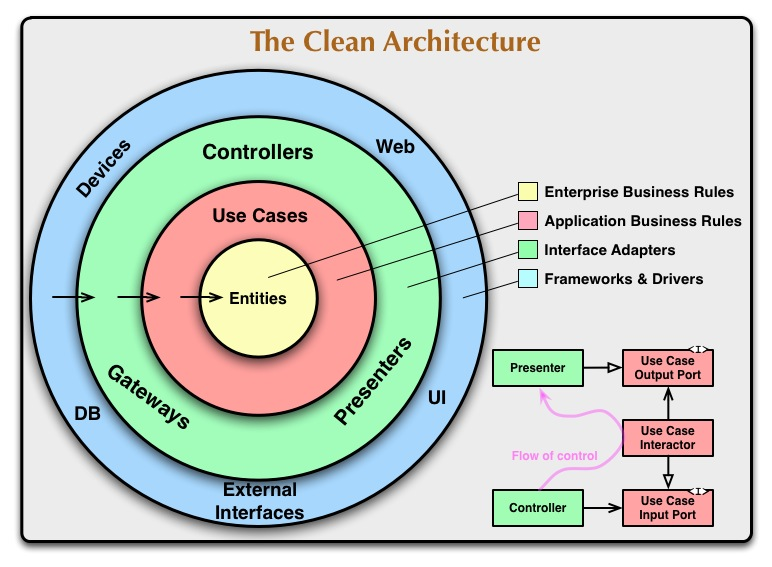
\includegraphics[width=1\linewidth]{assets/design/cleanarchitecture.jpg}
    \caption{The~Clean Architecture~\cite{a2021_clean_architecture_blog}}
    \label{fig:thecleanarchitecture}
\end{figure}

The~book~\cite{martin_2018_clean_architecture} explains multiple topics.
It discusses paradigms of programming: benefits and disadvantages of structured programming, object-oriented programming, and functional programming.
There is a~discussion about what these paradigms remove from developers, like assignments, goto statements, pointers, etc.
The~section about object-oriented programming brings a~dependency inversion, allowing dependency to point in the~inverted direction compared to the~flow of control.
The~dependency inversion principle is a~pillar of the~Clean Architecture, alongside the~single responsibility principle.
The~single responsibility principle states that every module should have only one reason to change, and therefore, that module should be responsible to only one actor.

There are more SOLID principles.
The~open-closed principle describes how entities should be open for an~extension rather than change.
The~Liskov substitution principle explains that extensions should be substitutable for their origin.
And interface segregation principle that explains that implementation of things that are not used should be avoided.

\begin{description}
    \item[Single-responsibility principle] \textcquote[p.~57--59]{martin_2018_clean_architecture}{An active corollary to 
Conway's law:\linebreak
The~best structure for a~software system is heavily influenced
by the \mbox{social} structure of the~organization that uses it so that
each software module has one, and only one, reason to change.}

\pagebreak

    \item[Open--closed principle] \textcquote[p.~57--59]{martin_2018_clean_architecture}{Bertrand Meyer made this principle famous\linebreak in~the~1980s.
The~gist is that for software systems to be easy to change,
they must be designed to allow the~behavior of those systems to be changed by~adding new code, rather than changing existing code.}

    \item[Liskov substitution principle] \textcquote[p.~57--59]{martin_2018_clean_architecture}{Barbara Liskov's famous definition of subtypes, from~1988.
    In short, this principle says that to build software systems from interchangeable parts, those parts must adhere to a~contract that allows those parts to be substituted one for another.}

    \item[Interface segregation principle] \textcquote[p.~57--59]{martin_2018_clean_architecture}{This principle advises software designers to avoid depending on things that they don't use.}

    \item[Dependency inversion principle] \textcquote[p.~57--59]{martin_2018_clean_architecture}{The~code that implements high-level\linebreak{}policy should not depend on the~code that implements low-level details.
Rather, details should depend on policies.}
\end{description}

\section{Client Application}
\label{design:client-application}

This section discusses the~design aspects of the~client application of the\linebreak{}designed game.
It discusses platforms that can be used and their limitations and benefits.
Then there is a~discussion on different options of frameworks to use according to platform specifications with extra pieces of information about the~selected framework and how it works.
Also, the~client architecture is described and designed according to previous chapters. 
And last but not least, the~state management selection and options discussion is done.

\subsection{Platforms}

The~designed game targets especially web and desktop platforms.
One of the~non-functional requirements is that it should be possible to extend the\linebreak{}game to other platforms, like mobiles.
The~web and desktop platforms are pretty similar.
They are both used on computers and use similar resolutions and workflow.
On the~other hand, the~mobile platform uses entirely different resolutions, and its users use their hands to control the~screen's content.
Mobiles also often have slow internet connections, and the~design of the~game for mobile in general and the~extension of the~game to mobiles in the~future should count with this.

For the~design of the~game \myAppName{}, the~development of an~application for the~web platform and the~desktop platform, targeting the~Windows operating system, will be considered.

\subsubsection{Cross-Origin Resource Sharing}

\begin{figure}
    \centering
    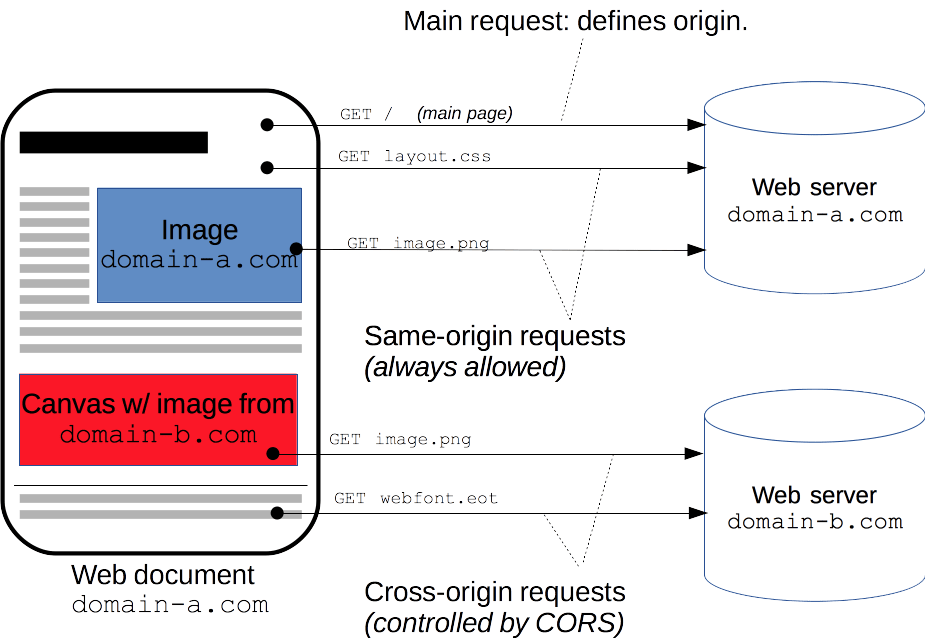
\includegraphics[width=1\linewidth]{assets/design/cors.png}
    \caption{The~CORS Mechanism~\cite{a2022_crossorigin}}
    \label{fig:design:cors-mechanism}
\end{figure}

The~web platform also has its limitations.
Modern web browsers include mechanisms that permit loading resources only from trusted client sources for security reasons.
When a~web application initiates a~\mintinline{js}{XMLHttpRequest} or uses the~Fetch API, a~browser requires that it must follow the~same-origin policy.
This mechanism is called CORS, and it means Cross-Origin Resource Sharing.

As stated in~\cite{a2022_crossorigin}, CORS is a~mechanism that lets servers specify trusted origins using HTTP headers.
Its purpose is to protect users and their cookies and other stuff stored in the~browser specifically.
Not enforcing the~same-origin policy could be a~potential risk for applications, e.g., banks that use cookies to verify that you are who you are, and using some malicious software attackers could dry out bank accounts.
That is not an~issue on desktop and mobile because cookies are stored inside applications' storage, and other\linebreak{}applications cannot access their cookies; therefore, these data can not be stolen.
The~essential idea from this concept is that this is not the~applications' fault; it is the~browsers' fault.
Servers set the~\mintinline{text}|Access-Control-Allow-Origin| header, and if matched with the~origin, a~browser allows the~application\linebreak{}to view and process its response.

The~header format \mintinline{text}/Access-Control-Allow-Origin: <origin> | */ must be used.
It can also be set with wildcards to relax the~CORS specification.
Communication between an~application and a~server with same-origin and cross-origin requests and their responses can be seen in the~figure~\ref{fig:design:cors-mechanism}.

\subsection{Frameworks}

It is often possible to use various libraries and frameworks to develop games and applications, making it easier to build software in terms of speed and capabilities.
Many experienced developers develop and optimize frameworks and develop an~efficient and versatile set of tools that allow developers who use these frameworks to take advantage of high-level functionality that addresses low-level functions such as security, component communication, dependency, and more.

Individual frameworks have different requirements and goals.
Some focus on specific programming languages, particular platforms, cross-platform mobile application development, and cross-platform development in general, whether it's mobile, web, or desktop.

Since the~developed game needs development for the~web, desktop (especially for the~Windows platform), and the~future possibility of extension to mobile devices, choosing one of the~cross-platform frameworks is necessary.
There are not many frameworks that support easy and stable development for both the~web and the~desktop and mobile devices.
Most frameworks, as mentioned, target a~single platform.
Some frameworks focus on the~development of applications or games for mobile devices, where they are further divided into development for Android and iOS~\cite{leler_2017_whats}.
They release SDKs (Software Development Kit) to develop on mentioned platforms, allowing developers to create widgets rendered to canvas and use native services.
Of course, this way does not allow the~creation of cross-platform software because of the~specificity of developing to the~individual platform, so they will not be considered.
There are also web frameworks that focus on robust web application development, which, in contrast, has an~actual usage even on mobile devices.

\begin{figure}
    \centering
    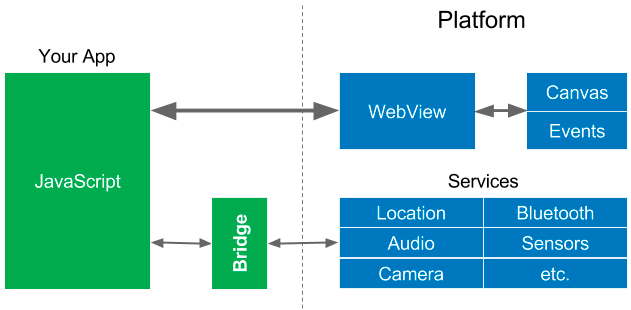
\includegraphics[width=1\linewidth]{assets/design/webview.png}
    \caption{WebView~\cite{leler_2017_whats}}
    \label{fig:design:webview}
\end{figure}

The~advantage of web frameworks over mobile ones, in terms of cross-platform development, is that thanks to technologies such as WebView and other supporting tools, it is possible to create a~mobile version of the~application.
Many cross-platform web frameworks use JavaScript with WebView, with a~design usually similar to the~figure~\ref{fig:design:webview}.
Representatives of these procedures are PhoneGap, Ionic, and other frameworks.
One of the~problems this approach has to solve is communication with device services such as cameras, Bluetooth, sensors, etc.
Therefore, the~so-called bridges, which communicate via JavaScript with native code, were most often created.

\begin{figure}
    \centering
    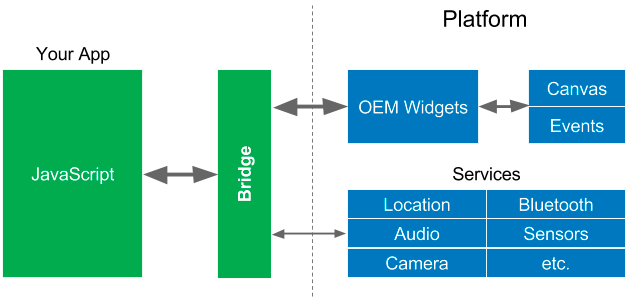
\includegraphics[width=1\linewidth]{assets/design/reactive.png}
    \caption{Reactive View~\cite{leler_2017_whats}}
    \label{fig:design:reactiveview}
\end{figure}

However, WebView does not perform well, so over time, other web frameworks have come up with different approaches.
One of these approaches is not to use WebView, but to use the~OEM (Original Equipment Manufacturer) widgets of the~platform directly for displaying~\cite{leler_2017_whats}.
One representative of this approach is React Native~\cite{a2022_react} with a design similar to the~figure~\ref{fig:design:reactiveview}.
It was created in 2015 by extending the~React web framework, both developed by Facebook~\cite{a2022_react}.
Unlike React, which uses web components, React Native uses OEM widgets.
OEM widgets are accessed from JavaScript using a~bridge that communicates with widgets and native platform services~\cite{leler_2017_whats}.
Both technologies are high-speed.
However, the~use of a~bridge causes a~communication bottleneck.
That causes a~slowdown in performance if a~lot of communication is done using the~bridge.
React Native has brought many benefits of reactive views to mobile applications.
React Native nowadays also focuses on developing for Windows, macOS, and the~web using React Native Windows, ReactNative macOS, and React Native Web~\cite{a2022_react}.
All mentioned projects use bridges to communicate with the~platform.

The~Flutter framework provides an~entirely different approach.
It has been historically developed as a~cross-platform framework for development on mobile devices.
Today, however, the~framework also supports development for the~web and desktops.
According to~\cite{leler_2017_whats}, unlike previous frameworks, which used web technologies to one degree or another, Flutter does not use JavaScript and web technologies to achieve better performance.
It uses custom widgets that are rendered to the~platform's canvas.
That also means that no matter the~operating system version, the~look and feel are always the~same because they do not rely on OEM widgets. 

\begin{figure}
    \centering
    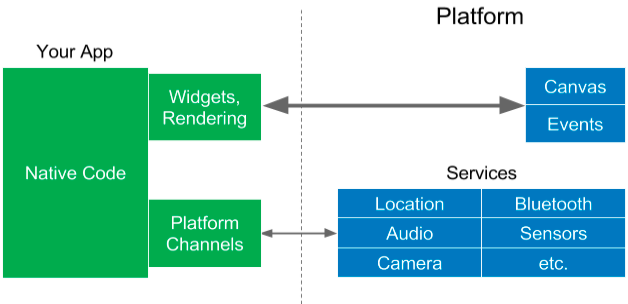
\includegraphics[width=1\linewidth]{assets/design/flutter.png}
    \caption{Flutter~\cite{leler_2017_whats}}
    \label{fig:design:flutterview}
\end{figure}

\subsubsection{Flutter}

Flutter is an~open-source framework developed by Google~\cite{a2022_flutter} that uses the Dart programming language, which allows the~ahead-of-time (AOT) compilation into native cross-platform code~\cite{leler_2017_whats}.
In addition, it allows the~just-in-time (JIT) compilation, which will enable developers to view changes almost instantly.
Compiling into native code provides many benefits, such as execution speed and performance.
\textcquote{leler_2017_whats}{The~fact that Flutter is the~only mobile SDK that provides reactive views without requiring a~JavaScript bridge should be enough to make Flutter interesting and worth trying, but there is something far more revolutionary about Flutter, and that is how it implements widgets.}
The~framework still needs to communicate with the~native platform.
The~platform channels interface is used for this purpose, as can be seen in~\ref{fig:design:flutterview}, which works on the~principle of data transfer.
The~framework encodes and decodes the~data, but overall the~whole process works faster than JavaScript bridges.

The~Dart language also contributed to the~significant improvement of Flutter 2, introducing sound null safety, which further helps Flutter type correctness and prevents null error crashes that can be caught during development~\cite{sells_2021_whats}.
This feature allows developers to use Flutter to write better and better code.
Flutter2 also introduced support for the~Add-to-app feature, enabling developers to use Flutter code inside their existing applications.

Flutter is very simple in principle.
It is designed to abstract its engine and framework from platforms, which will allow easy development on various platforms, as mentioned in~\cite{a2022_flutter_architecture}.
Platform-specific things are implemented, and the~rest of the~framework can remain unchanged, as seen in the~figure~\ref{fig:design:flutterlayers}.
No layer must interfere with the~layer below, and each part of the~system will design so that it can be replaced.
As described in~\cite{a2022_flutter_architecture}, the~embedder layer is written in the~languages appropriate for the~platform.
For Windows and Linux in C++, macOS and iOS in Objective-C or Objective-C++, and Android in Java and C++.
Embedder mediates communication with the~operating system, services, inputs, events, etc.
The~basics of Flutter are contained in the~engine layer, which is created primarily in C++.
The~engine is responsible for any rendering which uses the~Skia library.
The~Skia library is a~2D graphics library used as a~graphics engine, e.g., Google Chrome, Android, Flutter~\cite{skia_2022_skia}.
The~engine mediates the~framework using \mintinline{text}|dart:ui| libraries.
The~framework layer then provides access to a~reactive framework in the~Dart language\linebreak{}and provides a~range of widgets, layouts, gesture detectors, animation support, etc.
Developers usually use this layer.

A particular case is Flutter's web support~\cite{a2022_flutter_architecture}.
Flutter on the~web works with Dart's compiler, which compiles the~code into JavaScript.
Dart historically has a~significantly enhanced toolchain focused on compiling Dart code into JavaScript because Dart's first goal was to replace JavaScript in browsers.
Today some big applications like the~advertiser tooling for Google Ads use Dart to JavaScript compilation.
The~framework layer, written in Dart, will compile into JavaScript.
However, the~engine layer is written in C/C++; therefore, this layer cannot be used on the~web.
Similarly, it cannot use the~embedder layer to render as it is designed to run with the~operating system.
Flutter on the~web uses a~reimplemented version of the~engine above the~standard browser APIs.
This unique browser layer currently has two strategies to render.
\linebreak
It can use HTML mode to render HTML, CSS, Canvas, and SVG.
Or it can use WebGL mode, which uses CanvasKit, a~particular version of Skia library compiled to WebAssembly.
The~layers used in the~web version of Flutter can be seen in the~figure~\ref{fig:design:flutterweb}.

\begin{figure}
    \centering
    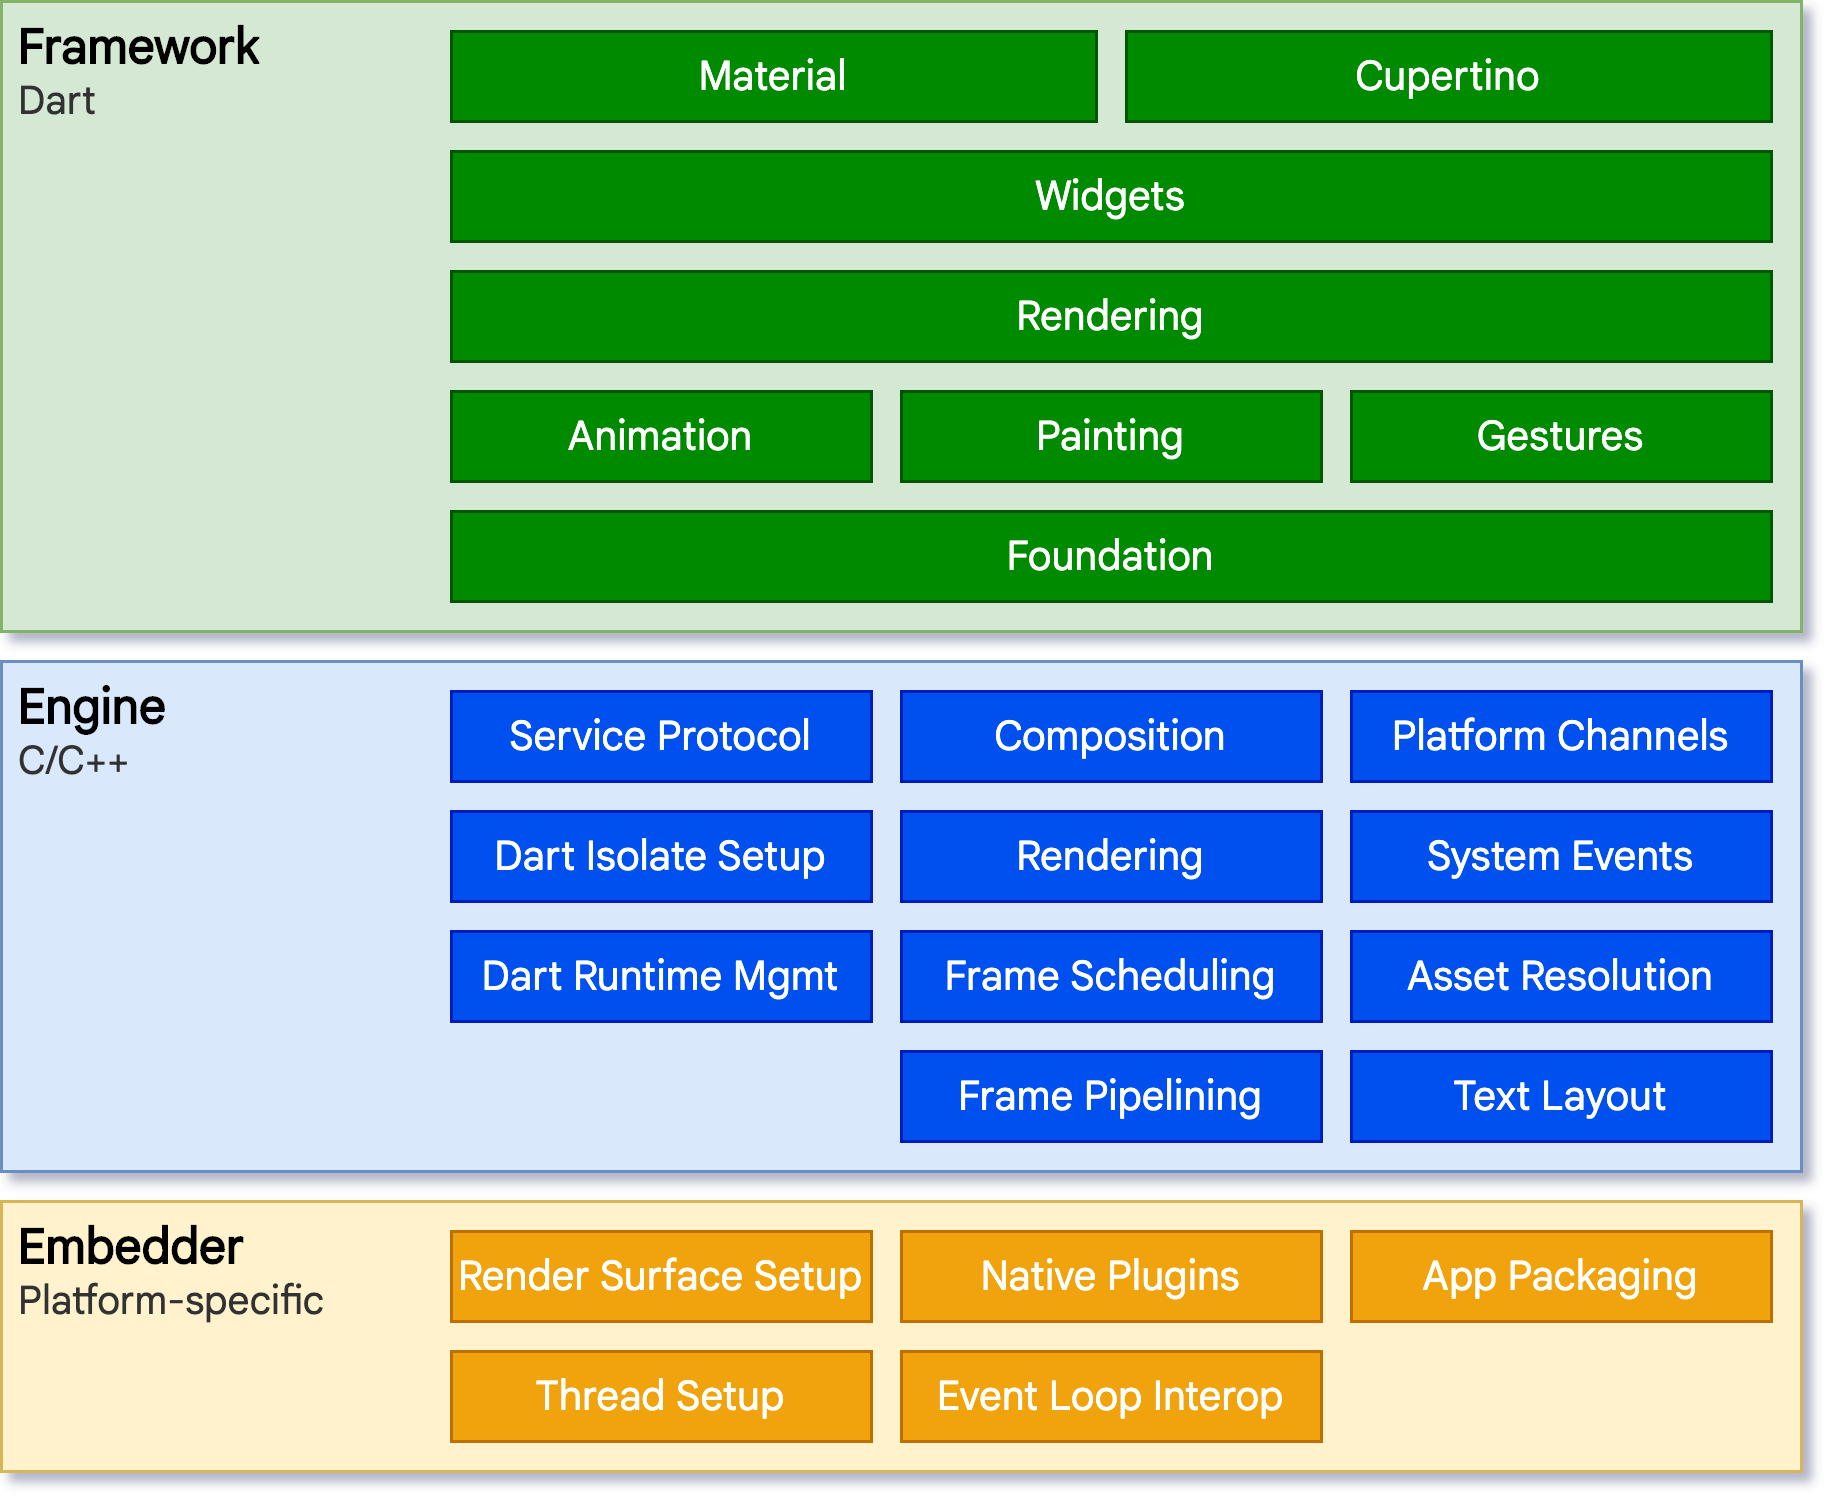
\includegraphics[width=1\linewidth]{assets/design/flutterlayers.png}
    \caption{Flutter's Architectural Layers~\cite{a2022_flutter_architecture}}
    \label{fig:design:flutterlayers}
\end{figure}

\begin{figure}
    \centering
    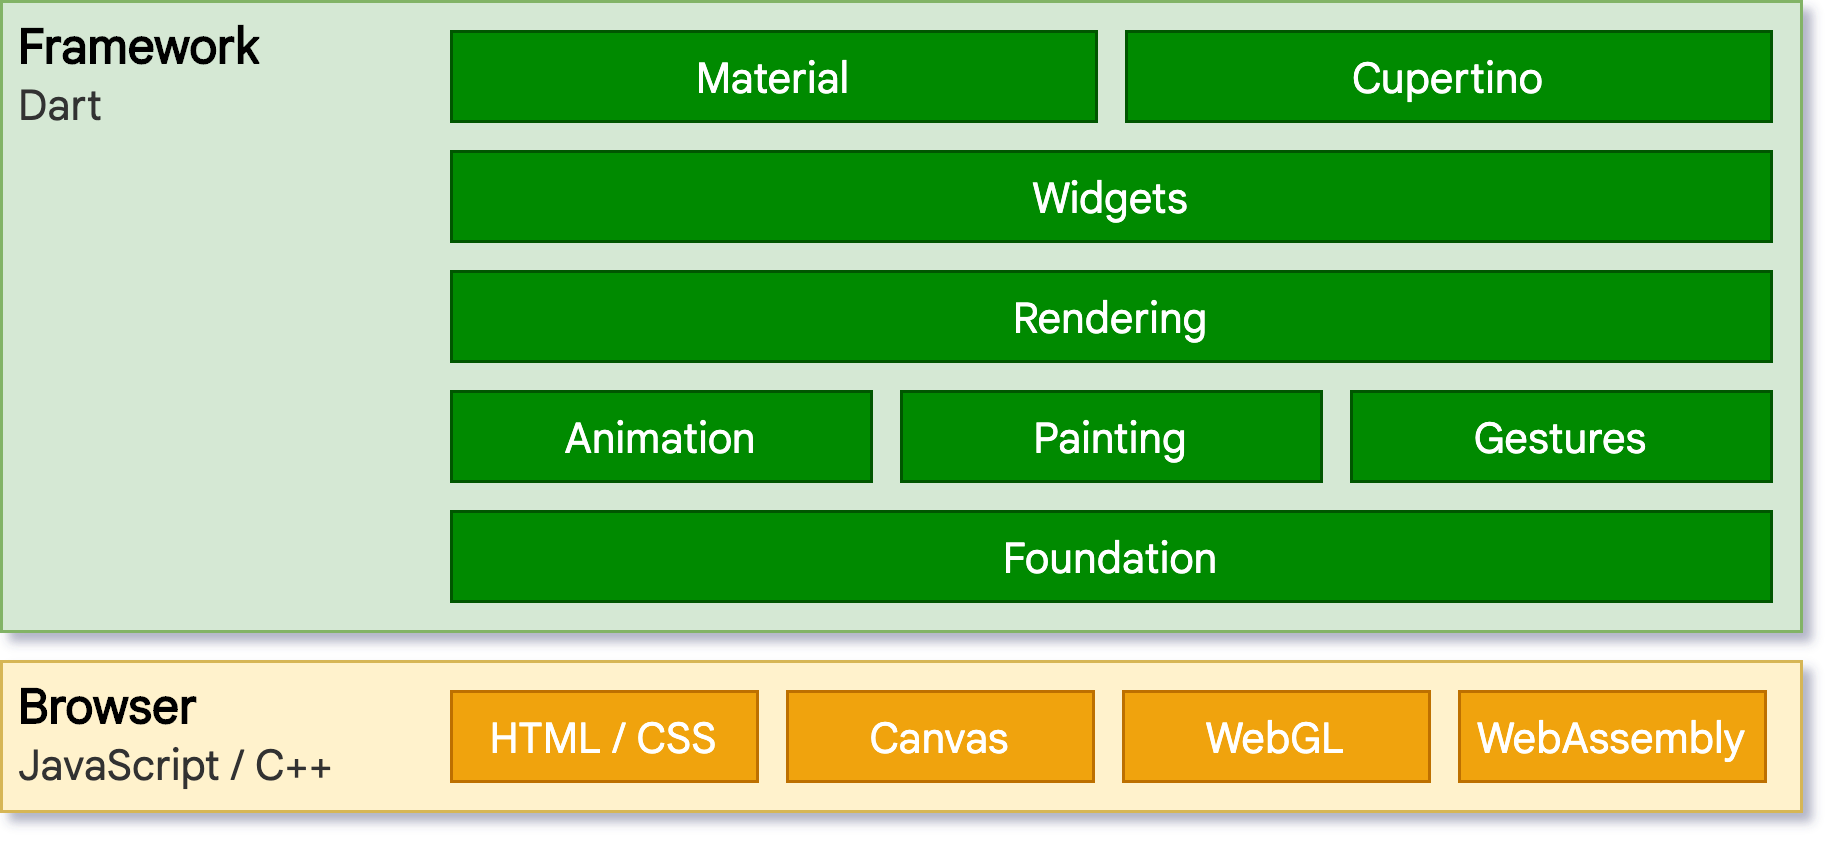
\includegraphics[width=1\linewidth]{assets/design/flutterweb.png}
    \caption{Flutter on Web~\cite{a2022_flutter_architecture}}
    \label{fig:design:flutterweb}
\end{figure}

\pagebreak

Widgets and Composition sections in the~Flutter documentation~\cite{a2022_flutter_architecture} also mention that Flutter uses widgets as building blocks of the~user interface.
Each widgets nests inside its parent, and together they form one hierarchy of widgets.
The~hierarchy of widgets also declares widgets' size, styles, or transformations.
Basic widgets are \mintinline{text}{Collumn} and \mintinline{text}{Row}, for layout of children widgets in a~collumn or a~row; \mintinline{text}{Stack} for stack-based layouts; and \mintinline{text}{Container} as a~generic purpose widget.
Widgets use composition rather than an~extension, and they are usually split into small single-purpose widgets.

The~framework uses two types of widgets: stateful and stateless~\cite{a2022_flutter_architecture}.
\linebreak
If the~widget does not change over time and therefore does not have a~state itself, the~\mintinline{text}{StatelessWidget} widget is used.
If the~widget changes its state, the~\mintinline{text}{StatefulWidget} is used.
Such a~widget is assigned a~unique \mintinline{text}{State}\linebreak{}object that holds the~state of the~widget, and the~widget must call \mintinline{text}{setState()} method each time its state changes and needs to be redrawn.
The~framework responds to the~call to this method and redraws it in the~next cycle.
Separating widgets into stateful and stateless improves application performance by not having to browse and render unchanged widgets.
In addition, thanks to a~separate state and widget, the~framework can support a~hot reload function, which allows the~app to rebuild widgets, i.e., appearance, but maintain the~state of the~respective widgets if they are in the~same place and the~framework can map them.

Whenever it is needed to redraw a~widget, its \mintinline{text}{build()} method is called.
Calling the~\mintinline{text}{build()} method, as mentioned in~\cite{a2022_flutter_architecture}, returns the~subtree of widgets according to which the~UI is rendered.
Because each widget can consist of others, a~tree of all widgets must be made recursively.
During this time, Flutter creates a~tree element that contains an~element for each widget.
\linebreak
The~element represents a~widget instance and represents either\linebreak{}the~element that participates in the~rendering (\mintinline{text}{RenderObjectElement})\linebreak{}or the~element that engages in composing the~hierarchy.
Another tree is created from this tree, a~tree that defines an~abstract model for layout and rendering consisting of the~general \mintinline{text}{RenderObject}.
During the~build phase, Flutter goes through the~\mintinline{text}{RenderObjectElement} in the~element tree and creates a~specific \mintinline{text}{RenderObject} for each.
Flutter traverses the~tree and transmits the~constraints downwards to determine the~layout, while the~descendants transmit their constraints, which must respect the~constraints.
This process can be seen in the~figure~\ref{fig:design:fluttertrees}.

\begin{figure}
    \centering
    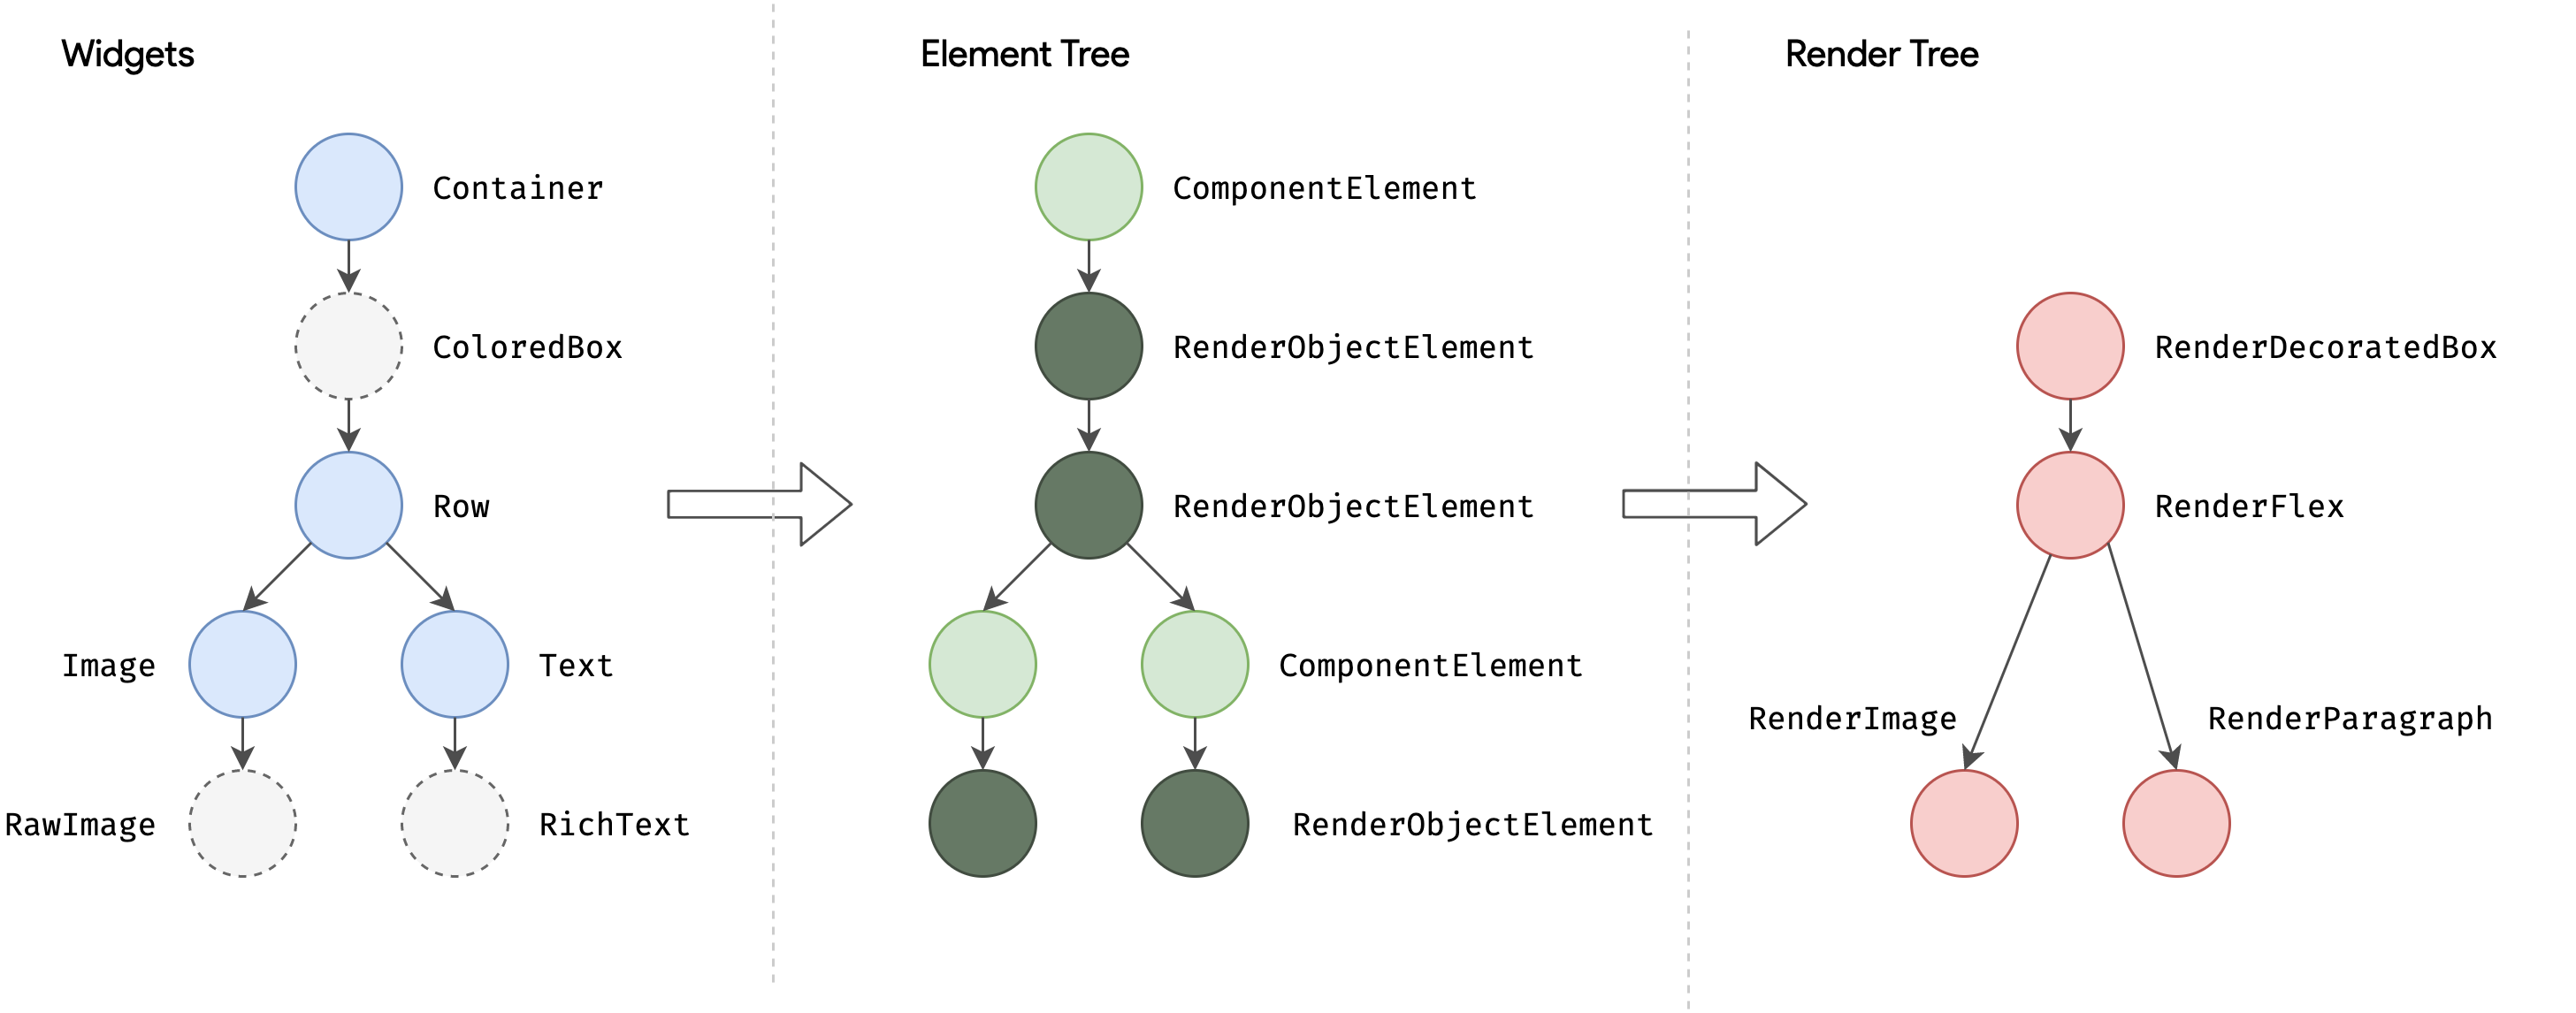
\includegraphics[width=1\linewidth]{assets/design/fluttertrees.png}
    \caption{Flutter Layout and Rendering~\cite{a2022_flutter_architecture}}
    \label{fig:design:fluttertrees}
\end{figure}

As mentioned, Flutter offers many benefits: compilation to native code, being able to compile using AOT and JIT, having a~fast performance, and much more.
It can also build for mobile platforms, desktops, and the~web.
That includes Android, iOS, Windows, Linux, macOS, and web.
Therefore, the~Flutter framework will be used to develop the~game.
With Flutter, the~game can be implemented as a~web version and a~Windows version (with a~Linux and a~macOS versions).
Also, it can be easily extended to mobile to provide an~Android and an~iOS version in the~future.
React Native would also be a~good choice, yet using JavaScript-based technology with its poor static analysis and dealing with other issues coming from the~JavaScript ecosystem is not preferable.
Therefore, Flutter was selected as a~better candidate.

\subsection{Architecture}

As mentioned in chapter~\ref{design:architecture:clean-archiecture}, the~client application should adhere to a~version of the~Clean Architecture.
Its layers should be divided into multiple layers: business contracts, business, data, and presentation.

\begin{figure}
    \centering
    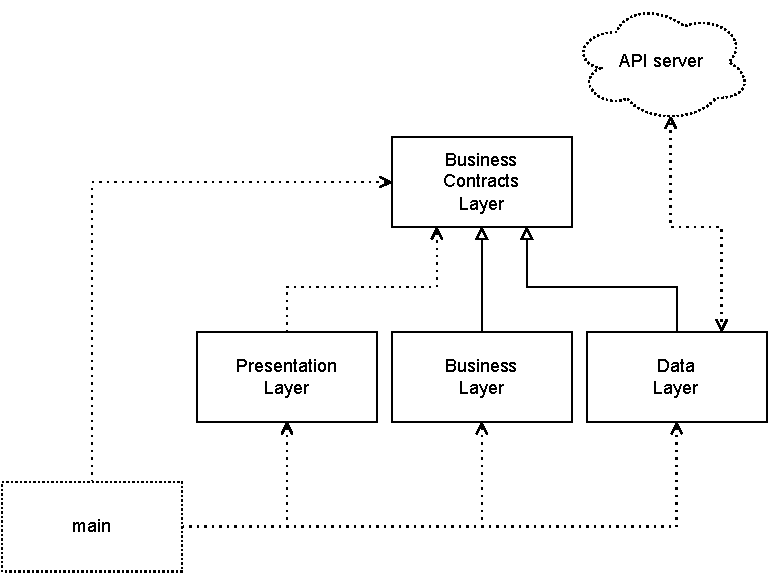
\includegraphics[width=1\linewidth]{assets/design/clientarchitecture.pdf}
    \caption{Client Architecture}
    \label{fig:design:clientarchitecture}
\end{figure}

The~business contracts layer contains entities and all contracts needed for services and repositories.
This layer describes the~interface that other layers use, and its interfaces do not contain any logic other than entities that can have a~simple entity modifying logic.
These layers should be isolated and should not use or know about any other layers.
It also should not use any external packages, especially with some logic.
It might use some external packages that help create interfaces or entities, nothing else.

The~business layer contains contracts implementations from the~business contracts layer, and it implements all services.
Some services might use contracts for repositories, but this layer does not implement those.
The~layer uses repositories' interfaces and gets specific instances as dependencies from constructors.

The~data layer contains implementations from the~business contracts layer, and it implements all repositories.
The~purpose of this layer is to implement repositories that communicate with the~API server.
Repositories are simple workers that process communication with the~external world.

And last but not least, the~presentation layer implements the~UI of the client application.
It uses services' contracts to request specific implementations by the~dependency injection tool registered with services and repositories in the~main method.
The~dependency injection tool provides repositories that are used by the~registered services.

The~main method registers all business contracts layer's interfaces to its dependency injection (DI) container and assigns them with specific implementations from business data layers.
Then it runs the~app.

\pagebreak

As can be seen from the~description and the~figure~\ref{fig:design:clientarchitecture}, the~client architecture follows the~SOLID principles, mainly the~dependency inversion principle. 

\subsection{State Management}

In order for the~client application design to be complete, it is necessary to determine how it will process its state.
That is possible by simple variables and passing up and down from the~widget to the~widget.
As can be seen, this would not be the~most efficient solution, especially since passing data from the~top widget to the~bottom ultimately would require passing data across multiple layers.
For this purpose, developers use state management procedures that allow data to be transferred differently.
Proper design and use of state management will also support the~sustainability and scalability of the~application, which is one of the~non-functional requirements.

Flutter is a~declarative framework~\cite{a2022_flutter_declarative}.
That means the~framework does not use an~imperative method to manage widgets and other framework parts, but rather the~framework expects that state changes, and the~framework then rebuilds and updates the~UI.
In other words, the~user interface is a~function of the~state.
This approach is atypical in many frameworks, such as the~Android SDK, and the~imperative method is often used.
The~declarative principle should also be maintained in state management.
Thanks to the~declarative approach, there is only one way to get to the~desired state, bringing many benefits.
On the~contrary, the~disadvantage of this approach is that it is initially non-intuitive.

According to~\cite{a2022_differentiate}, there can be several types of states in the~software.
And anything that is stored in memory at runtime could be considered a~state.
A better definition of states from an~architectural point of view is \textcquote{a2022_differentiate}{whatever data you need in order to rebuild your UI at any moment in time.}
States are often divided into ephemeral and app states.

An ephemeral state, also often referred to as a~UI state, is a~state that is relevant to only one widget, and only that widget works with it~\cite{a2022_differentiate}.
In this case, there is no need for the~state to be shared in any way with other parts of the application, as this would add unnecessary communication and the~need for more complex logic.
An example of such a~state can be the~current navigation tab.
For an~ephemeral state, it is enough to use the\linebreak{}\mintinline{text}{StatefulWidget} widget and use the~\mintinline{text}{setState()} method to notify the~widget and then redraw it.

In contrast, the~app state, sometimes referred to as the~shared state, is part of several parts of the~application~\cite{a2022_differentiate}.
So this state is trivially not ephemeral.
App state needs more complex management because it is used by multiple parts of the~application, which are often independent and far apart.
The~choice of the~appropriate type of management for such a~state depends on the\linebreak{}complexity of the~application.
An example of an~app state can be the\linebreak{}management of information about a~logged-in user, a~shopping cart in an \mbox{e-shop}, settings, etc.

Whether to use ephemeral or app state may not always be clear.
\linebreak
Ephemeral states can also be used outside the~widget by passing callbacks; however, if a~callback is passed more than one level, it will probably be possible to use another solution.
\textcquote{a2022_differentiate}{The~rule of thumb is: Do whatever is less awkward.}
Some of the~most used state management tools are MobX, Redux, and BLoC.

\subsubsection{MobX}

MobX is a~state management library with three concepts: Observables,\linebreak{}Actions, and Reactions~\cite{a2022_mobxdart}.
This is an~implementation of the~observer \mbox{pattern}.
Concepts are simple in nature and have a~fast learning curve.
According to~\cite{a2022_mobxdart}, the MobX library uses the~following concepts:

\begin{description}
    \item[Observables] Represent states in the~form of any object with data, from numbers to complex objects.
    Data are reactive, which means that each change will notify each observer.
    \item[Actions] Describe changes in the~states of observables. Observables can be changed directly, but actions add semantic meaning, so instead of calling \mintinline{text}{value++} directly, the~\mintinline{text}{increment()} action should be called. The~action triggers a~state change.
    \item[Reactions] Automatically monitor state changes. a~reaction is made immediately after each change.
\end{description}

\subsubsection{Redux}

Redux is a~predictable and centralized state container.
It is one of the~most known libraries on state management.
According to~\cite{brianegan_2021_fluttercommunityreduxdart}, it works with three concepts: Actions, Reducers, and Store:

\begin{description}
    \item[Actions] Represent information sent from the~application to the~store and are its only data source.
    \item[Reducers] Describe how the~application state changed in response to actions.
    Reducers must be pure, which means they must not use non-pure functions and do not mutate the~state; they create a~new copy.
    \item[Store] Represents an~object that holds the~application state.
    It also provides the~current state and sets up the~initial state.
\end{description}

\subsubsection{BLoC}

The~Business Logic Component (BLoC) is not a~library but a~design pattern.
This pattern consists of simple rules that each implementation must follow, leaving specific implementation elements to developers.
According to~\cite{paolosoares_2018_flutter} these design rules are:

\begin{enumerate}
    \item Inputs and outputs are simple
    \mintinline{text}|Stream|/\mintinline{text}|Sink| only.
    \item Dependencies must be injectable and platform agnostic.
    \item No platform branching allowed.
    \item Implementation can be whatever you want
    if you follow the~previous rules.
\end{enumerate}

BLoC also has rules for UI design.
These rules describe the~relationship between the~UI component and the~BLoC component.
According to~\cite{paolosoares_2018_flutter} these rules are:

\begin{enumerate}
    \item Each \textquote*{complex enough} component has a~corresponding BLoC.
    \item Components should send inputs \textquote*{as is}.
    \item Components should show outputs as close as possible to \textquote*{as is}.
    \item All branching should be based on simple BLoC boolean outputs.
\end{enumerate}

This design pattern was created to separate code with logic
from platform-specific dependencies~\cite{paolosoares_2018_flutter}.
In contrast to the~Redux library, the~BLoC pattern works with multiple state stores.

There is a~Bloc library by Alex Angelov for Dart language that implements the~BLoC pattern~\cite{angelov_2022_bloc}.
It tries to implement the~rules described above using the~\mintinline{text}{Stream} and \mintinline{text}{Sink} classes, which allow asynchronous communication.
In addition, this library provides unique Flutter widgets that help listen to changes and rebuild widgets.
This library works with four basic concepts: Events, States, Transitions, Blocs.
In parallel, the~library also provides a~version called Cubit, which works with functions instead of events.
That allows events to be triggered synchronously using functions instead of adding an~event to the~Stream.
Cubit can be easier for smaller applications that can handle more straightforward logic.
According to~\cite{angelov_2022_bloc}, the Bloc library uses the\linebreak{}following concepts:

\pagebreak

\begin{description}
    \item[Events] Represent events in the~form of any object.
    It is the~only input that comes inside the~Bloc.
    \item[States] Represent states in the~form of any object.
    \item[Transitions] Describes the~transition from one state to another, consisting of the~current state, the~next state, and the~triggered event.
    \item[Blocs] Represent classes extending the~Bloc class.
    They accept events, output states, and handle transactions.
    Blocs register event handlers using \mintinline{text}{on<Event>()} methods used in the~constructor.
\end{description}

\subsubsection{Evaluation}

Sending states and callbacks through several levels of widgets is not suitable, so it is not even considered for state management.
Although the~MobX library offers simple concepts and less boilerplate due to code generation, code generation may be slower.
The~Redux and Bloc libraries seem to be similar.
Both work with data asynchronously, but implementations are different.
The~most significant difference is that Redux has only one source of state, while there are multiple in Bloc.
In Redux, only parts of the~states change.
In Bloc, on the~other hand, the~whole state constantly changes.
However, it is small enough and understandable, so it does not cause any problems.
The~Bloc library will be used to develop the~designed game, which will enable an~easy and robust solution thanks to its asynchronous design.

\section{Server Application}

This section discusses the~design aspects of the~server application of the~designed game.
It discusses the~design of an~API server.
Then the~server architecture is described and designed according to previous chapters.
There is a~discussion on different framework options and how the~framework works with entities and DTOs.
Then there is a~discussion about controllers, repositories, and services.
And finally, a~note about tokens.

\subsection{Web API}

Application Programming Interface (API) is an~interface with a~set of functions that can be used to get data from an~application~\cite{a2022_aspnet}.
API accessed over the~web using the~HTTP protocol is called Web API.
They can be developed with different technologies like ASP.NET, Java, Python, etc.
A web API can be used from a~mobile, desktop, web, or any other application or game using the~HTTP protocol.
Web API can also use other web APIs.

One of the~representatives of web API is ASP.NET Web API~\cite{a2022_aspnet}.
\linebreak
It is a~web framework that is often used to create websites and APIs using languages such as C\#.
The~framework supports an~automatic serialization of data classes into the~JSON format.
It supports built-in support for authentication and authorization with built-in support for standards such as JSON Web Tokens (JWT).
It also provides multiple annotations for use inline with the~code, like routing annotations that let developers mark methods that should provide routing.

The~ASP.NET Web API framework will be used in the~server part of the~designed game for its simplicity and industry-level power.

\subsection{Architecture}

As mentioned in chapter~\ref{design:architecture:clean-archiecture}, the~server application will follow the~principles mentioned in the~Clean Architecture.
It is divided into multiple layers: data layer, repositories contracts layers and repositories layer, services contracts layer and services layer, and controllers layers.

\begin{figure}
    \centering
    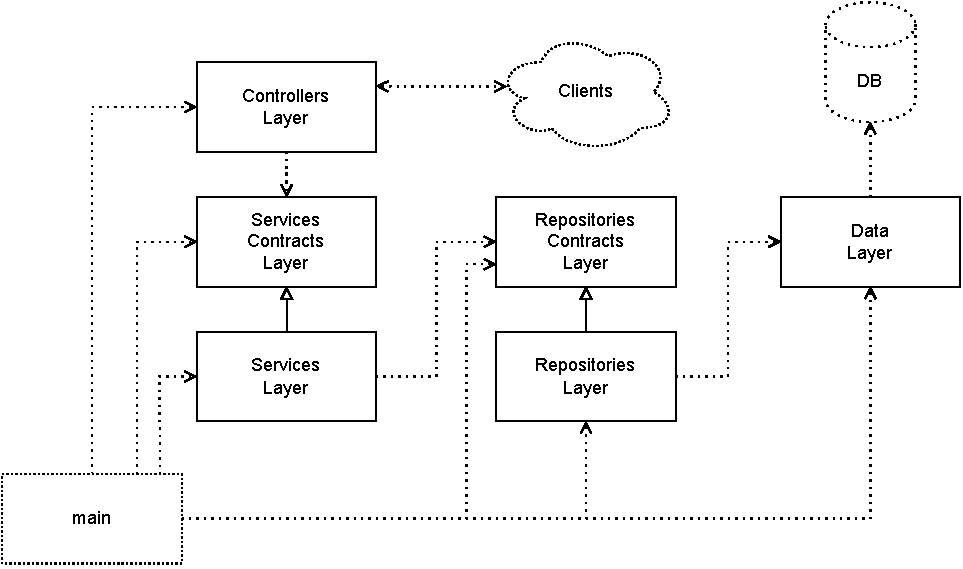
\includegraphics[width=1\linewidth]{assets/design/serverarchitecture.pdf}
    \caption{Server Architecture}
    \label{fig:design:serverarchitecture}
\end{figure}

The~data layer declares entities and their mapping.
Entities should use Object-Relational Mapping (ORM) to map themselves to the~database model.
Using the~ASP.NET and its Entity Framework, setting up entities and mapping is very straightforward.
The~Entity Framework recognizes the~primary identification and translates all attributes and their types to corresponding database types.

The~repositories contracts layer contains repositories' interfaces.
They are used to provide basic methods for communication with the~database.
These interfaces do not use any code from other layers.

The~repositories layer contains the~repositories contracts layer's implementation of the~repositories.
These implementations return Data Transfer Objects (DTOs) after processing entities fetched from the~database.

The~services contracts layer contains services' interfaces.
They are used as a~layer between controllers and repositories.
These interfaces do not use any code from other layers.

The~services layer contains the~services contracts layer's implementation of the~services.
These implementations use repositories contracts passed in their constructors using the~dependency injection.

The~controllers layer provides Web API controllers that processes work using services.

As you can see from the~description and the~figure~\ref{fig:design:serverarchitecture}, the~server architecture follows the~SOLID principles, mainly the~dependency inversion principle.

\subsection{Entities and DTOs}

The~Entity Framework is an~open-source data access framework.
It does Object-Relational Mapping (ORM), so developers can use the~database as with objects~\cite{a2021_overview}.
The~framework also reduces the~direct data access needed and exposes a~high-level interface.

The~database model consists of entities and the~database context object~\cite{a2022_creating}.
The~context object represents the~database relations.
Entities are ordinary data objects.
Each entity is registered as \mintinline{text}|DbSet<Entity>| attribute with a~getter and a~setter.
The~context can set up entity mappers using the~Fluent API, as can be seen in the~code~\ref{fig:database-context}.
The~Fluent API is a~method of modifying the~model without changing the~entity class.
It also has higher precedence than annotations that can be used directly on entity class and its attributes.

\begin{listing}
    \caption{Sample Database Context}
    \label{fig:database-context}
    \begin{minted}{csharp}
internal class MyContext : DbContext
{
    public DbSet<User> Users { get; set; }

    protected override void OnModelCreating(
        ModelBuilder modelBuilder
    )
    {
        modelBuilder.Entity<User>()
            .HasIndex(u => u.Username)
            .IsUnique();
    }
}
    \end{minted}
\end{listing}

Querying data from the~database with the~Entity Framework can be done using the~Language-Integrated Query (LINQ).
LINQ queries are strongly typed, and it is as simple as calling methods in the~database context.
Because methods returns live queries, it is recommended to await the~query as a~collection to finish the~fetching.

Entities are mapped from the~database.
Entities are transformed into Data Transfer Objects (DTO) to handle incoming and outcoming data.
DTOs always contain only data needed for further processing to prevent sending unnecessary data.

The~typical scenario flow might be that a~controller is triggered, it calls a~service, which calls a~repository.
The~repository does a~fetch to the~database, and data are stored in a~collection and later transformed into DTOs.
DTOs are returned from the~repository and processed by the~service.
After processing, the~data are returned to the~controller, creating a~response containing those data.

\subsection{Controllers}

Controllers provide Web APIs that process requests using services from the services layer delivered to the~services contracts layers using the~dependency injection tool.
Controllers should be designed to cover all use cases of the developed game.

There should be a~controller for the~authentication of users.
That means signing in and signing up for the~game.
These API endpoints should be allowed to be run anonymously.
If the~sign-in or sign-up processes finish successfully, a~JWT token should be generated and returned as a~response with user data.

The~user controller should contain endpoints to get a~user by id, get a~user by username and get a~user by the~token.
These endpoints should be locked and available only to authenticated users.
Each endpoint should return a~user object.

The~story controller should be able to get all stories and a~story by its id.
Based on the~endpoint, different data should be returned.
The~get-all-stories endpoint should return a~list of stories.
The~get-story-by-id endpoint should return a~story with all of its missions.
These endpoints should be locked and available only to authenticated users.

Similarly, the~mission controller should also be able to get all missions and a~specific mission.
Both endpoints return game, learning, or storytelling mission.
Additionally, it should also have an~endpoint to update the~game result.
These endpoints should be locked and available only to authenticated users.

\pagebreak

And finally, the~stats endpoint should return stats for all stories and their mission for the~authenticated user.
This endpoint should be locked and available only to authenticated users.

\subsection{Services}

Services handle requests from controllers.
They are the~middleware between controllers and repositories and handle additional logic.
There should be three types of services: a~user service, a~story service, and a~token service.

The~user service should be able to get a~user by their id or username.
\linebreak
It should also process login and register processes.
This service should also know how to hash and verify users' passwords.

The~story service should contain methods to get story and stories, mission and missions, and save game progress.
Their URL attribute differentiates the~mission and the~story.
If requesting all missions, a~story URL must be provided.
All stories do not need additional data.

The~token service needs to contain the~generation of a~token and its\linebreak{}verification.
The~token is generated based on the~user data object.
And the~verification is done by passing the~token.

\subsection{Repositories}

There should be at least two repositories for stories and users.
The~user repository should contain creating a~new user and getting a~user by their id or username.
The~story repository should contain all methods to fetch and modify stories and missions.
Getting all stories, getting a~specific story by its story URL, getting all missions by their story URL, and getting a~particular mission by its URL.
It should also provide getting stories' stats for a~user.
And the~save game progress.

\subsection{Tokens}
\label{design:server:tokens}

User authentication is done either by sessions or tokens.
These two methods do a~similar job, but servers manage sessions, and clients manage tokens.
Both methods can deal with authentication and authorization.
Authentication verifies that a~user is who they say they are.
That can be done by providing a~password or a~fingerprint.
Authorization verifies that a~user has permission to do things.
It is a~way to allow a~user to access some locked resource.~\cite{lin_2018_tuck}

Tokens deals with the~authorization of APIs.
Typically JSON Web Tokens (JWT) are used to secure APIs.
JWT is an~open security standard that allows the~secure transmission of data~\cite{lin_2018_tuck}.
JWT is added to an~authorization header \mintinline{text}|Authorization: Bearer <jwt-token>| on the~client's request, and the~server then reads it and verifies it.
A schema of JWT lifetime can be seen in the~figure~\ref{fig:design:jwt}.

\begin{figure}
    \centering
    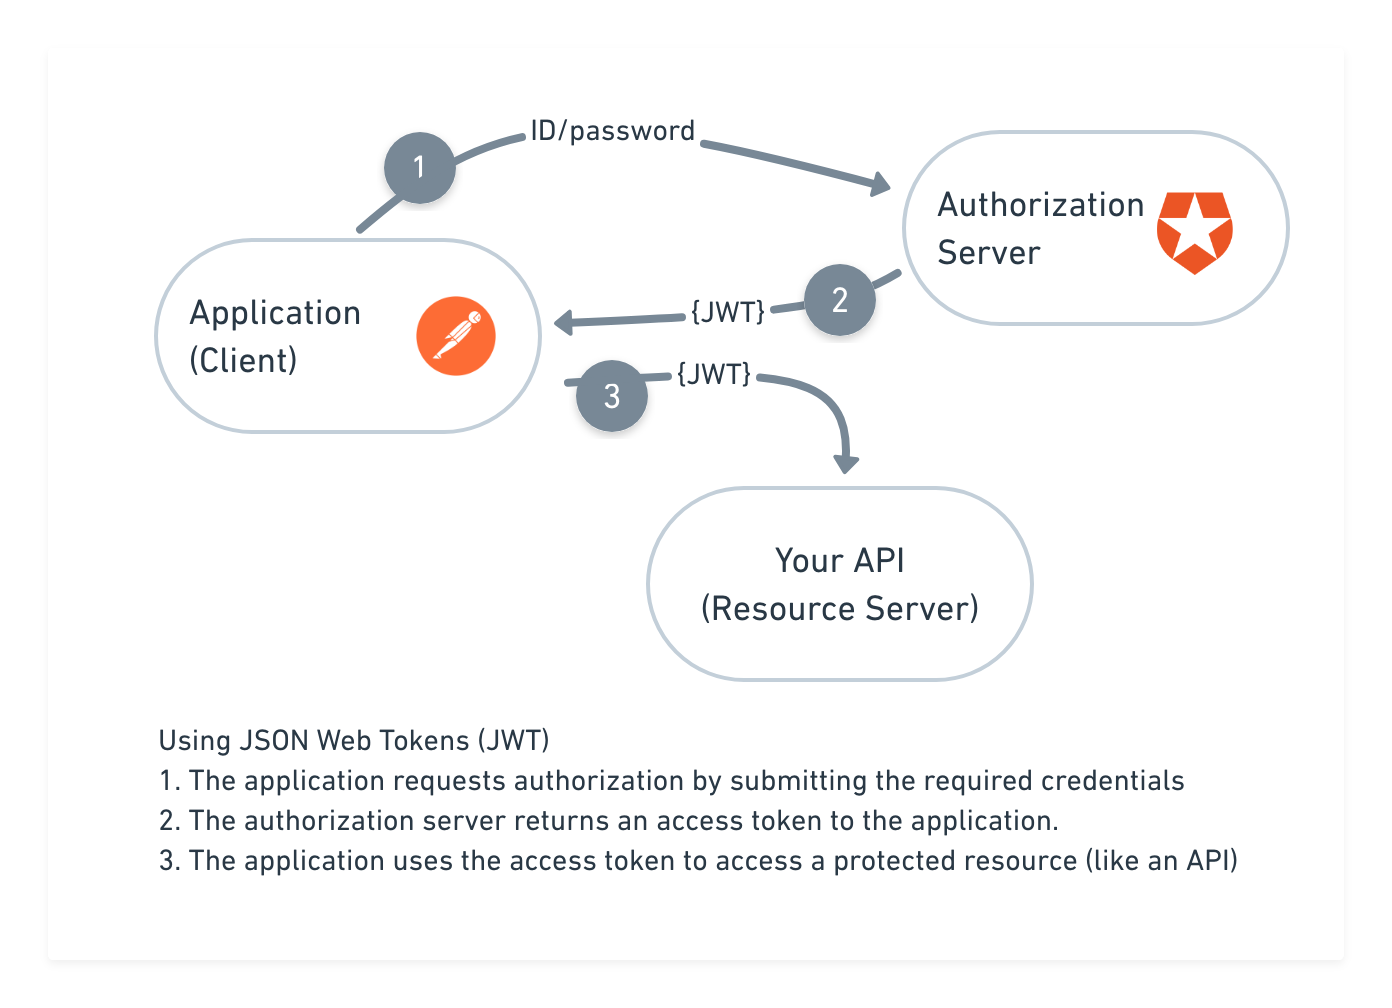
\includegraphics[width=1\linewidth]{assets/design/jwt.png}
    \caption{JSON Web Tokens~\cite{lin_2018_tuck}}
    \label{fig:design:jwt}
\end{figure}

Users will be forced to sign in using their username and password combinations to authenticate.
The~game verifies that the~user is who they say they are.
Then, the~game saves the~JWT token from the~response, and from now on, it uses the~token to authorize the~request to the~Web API.

\section{Database}

In this section, there are discussions about types of databases, SQL vs. NoSQL, inheritance, and conceptual schema.

A database is a~collection of data stored in a~system.
They are used for the~persistent storage of information from applications.
According to software requirements, the~data is well-organized and offers many advantages over simple file storage, such as fast search and querying.

According to~\cite{a2018_difference_db}, one of the~most critical decisions is choosing the~right type of database and the~correct database system.
Databases can be relational (SQL) and non-relational (NoSQL).

Relational databases mainly use the~SQL (Structured Query Language) language.
It is a~declarative query language that allows performing complex queries~\cite{a2018_difference_db}.
In SQL databases, data are structured, and it is based on ACID principles: atomicity, consistency, isolation, and durability.
Their scheme is fixed.
SQL databases are vertically scalable, which means increased RAM, CPU, or SSD performance.
An example of such a~database is PostgreSQL.

Non-relational databases are of many kinds and types.
They have a~dynamic schema and are suitable for hierarchic data storage~\cite{a2018_difference_db}.
NoSQL databases are horizontally scalable, allowing to handle a~more significant amount of workload by using another server.
These databases are based on CAP: consistency, availability, partition tolerance.
Examples of NoSQL databases are Neo4j and MongoDB.

Because the~data for the~developed game are with a~fixed schema, using a~SQL database is more than suitable.
The~game will use the~open-source database PostgreSQL.

\subsection{Conceptual Schema}
\label{design:conceptual}

To create a~database, creating a~conceptual schema is a~good choice.
A conceptual schema is a~schema that models only the~relations between entities.
Entities have attributes, but they do not have a~type.
An essential part of the~schema is the~relations, which can have different cardinality and partiality.

The~designed schema has six entities: \mintinline{text}|User|, \mintinline{text}|Story|, \mintinline{text}|Mission|, \linebreak\mintinline{text}|Game_mission|, \mintinline{text}|Learning_mission|, and \mintinline{text}|Game_progress|.
The~schema can be seen in the~figure~\ref{fig:design:conceptualschema}.

The~\mintinline{text}|User| entity has primary key \mintinline{text}|id| and attributes \mintinline{text}|name|, \linebreak\mintinline{text}|password|, \mintinline{text}|username|, and \mintinline{text}|description|.
The~\mintinline{text}|username| attribute is unique.

The~\mintinline{text}|Story| entity has primary key \mintinline{text}|id| and attributes \mintinline{text}|url|, \mintinline{text}|name|, and \mintinline{text}|description|.
The~\mintinline{text}|url| attribute is unique.

The~\mintinline{text}|Mission| entity has primary key \mintinline{text}|id| and attributes \mintinline{text}|url|, \mintinline{text}|name|, \linebreak\mintinline{text}|description|, and \mintinline{text}|order|.
The~\mintinline{text}|url| attribute is unique.

The~\mintinline{text}|Game_mission| entity extends entity \mintinline{text}|Mission| and has attributes \linebreak\mintinline{text}|commands_initial|, \mintinline{text}|board_initial|, \mintinline{text}|board_result|, \mintinline{text}|speed_limit|, \linebreak\mintinline{text}|robot_initial|, \mintinline{text}|robot_result|, and \mintinline{text}|task_description|.

The~\mintinline{text}|Learning_mission| entity extends entity \mintinline{text}|Mission| and has attributes \mintinline{text}|data|, and \mintinline{text}|is_story|.

The~\mintinline{text}|Game_progress| entity has primary key \mintinline{text}|id| and has attributes \mintinline{text}|commands|, \mintinline{text}|speed|, \mintinline{text}|size|, and \mintinline{text}|completed|.

From the~relations, the~\mintinline{text}|Story| entity can have multiple \mintinline{text}|Mission|s.
The~\mintinline{text}|User| entity and \mintinline{text}|Game_mission| can have multiple \mintinline{text}|Game_progress|.

\begin{figure}
    \centering
    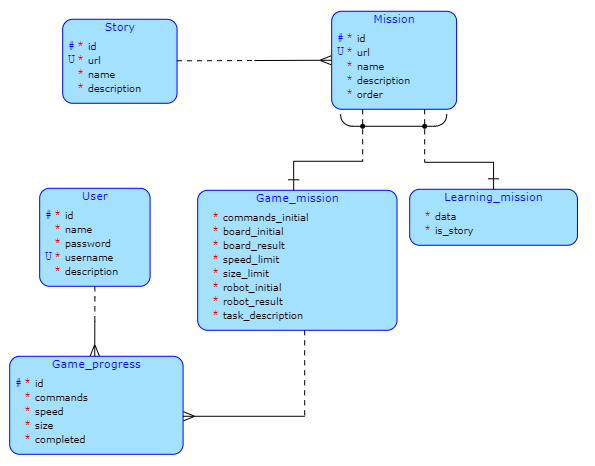
\includegraphics[width=1\linewidth]{assets/design/conceptualdiagram.png}
    \caption{Conceptual Schema}
    \label{fig:design:conceptualschema}
\end{figure}

\subsection{Inheritance}

In the~conceptual schema, inheritance is used.
Inheritance can be solved with three different approaches.

The~first approach is a~table per hierarchy~\cite{a2010_enterprise}.
This approach denormalizes the~schema and joins all tables into one.
A column that determines a~type of data is added to the~schema.
That means only one table per hierarchy is created.

The~second approach is a~table per type~\cite{a2010_enterprise}.
This approach uses tables from all entities.
There is a~foreign key to the~base table in children's tables.
Even abstract classes have their tables.
And children's tables contain only non-inherited properties.

The~third approach is a~table per concrete type~\cite{a2010_enterprise}.
This approach is similar to the~table per type, but it does not create tables for abstract classes.

Determining what approach is the~best is a~matter of specific needs.
In the~developed game, the~second approach will be used~-- the~table per type.
That means no attributes will be duplicated, and all hierarchy will be preserved.

\section{User Interface}
\label{design:ui}

In this section, a design of wireframes will be discussed.

\subsection{Sign In and Sign Up Screens}

\begin{figure}
    \centering
    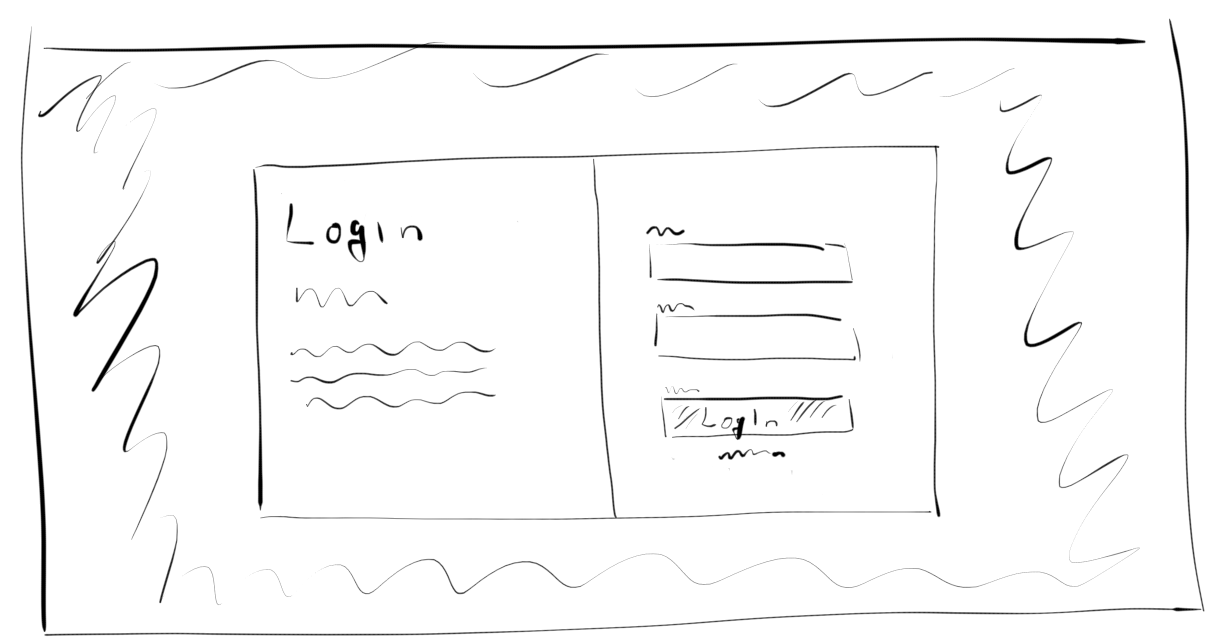
\includegraphics[width=1\linewidth]{assets/design/ui/wir_login.png}
    \caption{Sign In Wireframe}
    \label{fig:design:wir:login}
\end{figure}

On the screen, \ref{fig:design:wir:login} will be one of the important components -- sign in and sign up.
If the user does not register or log in, he cannot play the game.
Therefore, it will be more than appropriate if the screen is simple and contains a meaningful design.

The screen contains text inputs for entering nicknames, passwords, and more and includes a button that is used to submit the form.

\subsection{Missions Screen}

Missions screen \ref{fig:design:wir:missions} is a transition screen for selecting missions to play.
It contains a top menu from which it is possible to access all stories, statistics, a profile, and a button on the main page.

It contains an overview of individual missions, tuned into a linear sequence, but it is also possible to make a divided linear sequence of missions.
A line is displayed between the missions, indicating continuing to the next mission.
Next to the mission is its name.

\begin{figure}
    \centering
    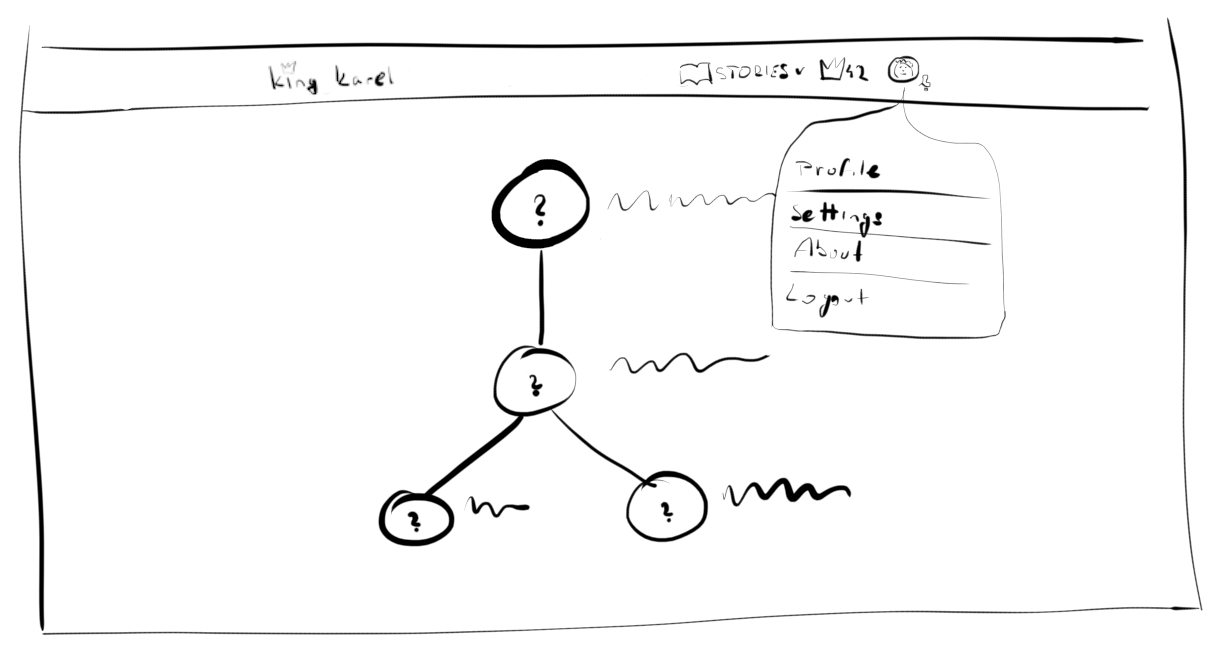
\includegraphics[width=1\linewidth]{assets/design/ui/wir_stories.png}
    \caption{Missions Wireframe}
    \label{fig:design:wir:missions}
\end{figure}

\subsection{Story Screen -- Game}

Story screen with click on a game mission on figure \ref{fig:design:wir:story-game}.
The click will show a bubble dialog that contains information about the number of points completed, the mission name, the caption, and the play button.

\begin{figure}
    \centering
    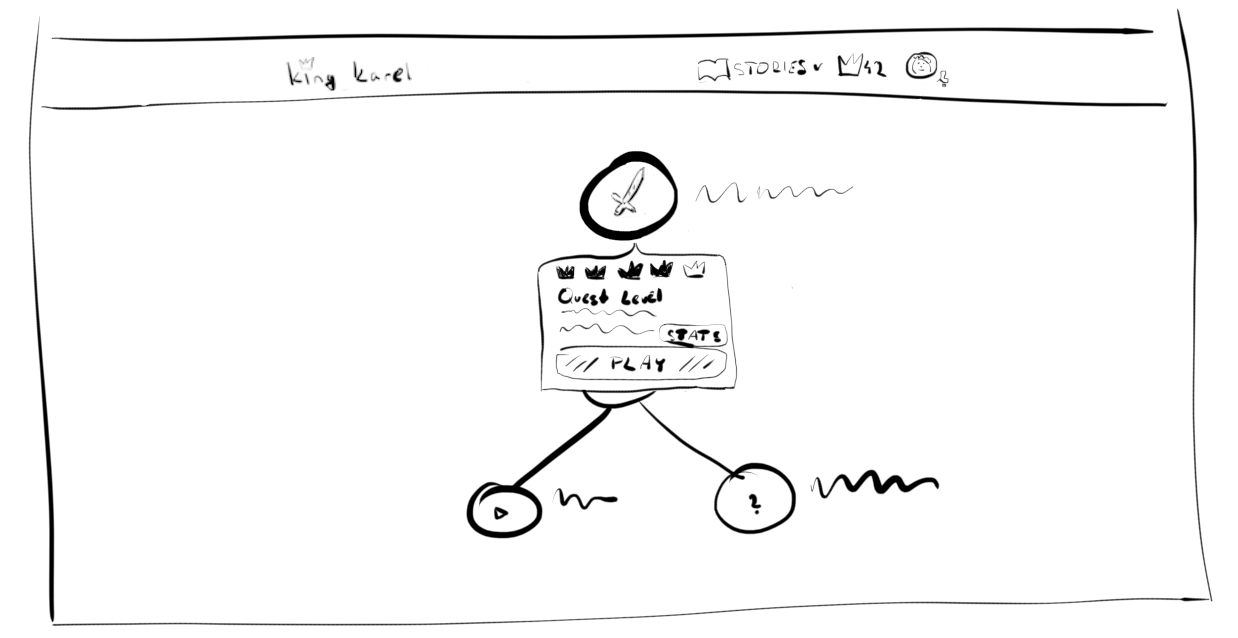
\includegraphics[width=1\linewidth]{assets/design/ui/wir_game.png}
    \caption{Game Mission Wireframe}
    \label{fig:design:wir:story-game}
\end{figure}

\subsection{Story Screen -- Learning and Storytelling}

Like the previous wireframe, on figure \ref{fig:design:wir:story-learning} there is a story screen which, after clicking on the learning mission or storytelling mission, displays a bubble dialog with information about the learning mission or storytelling mission.
It contains information about the title, description, and a button to start a learning or storytelling mission.

\begin{figure}
    \centering
    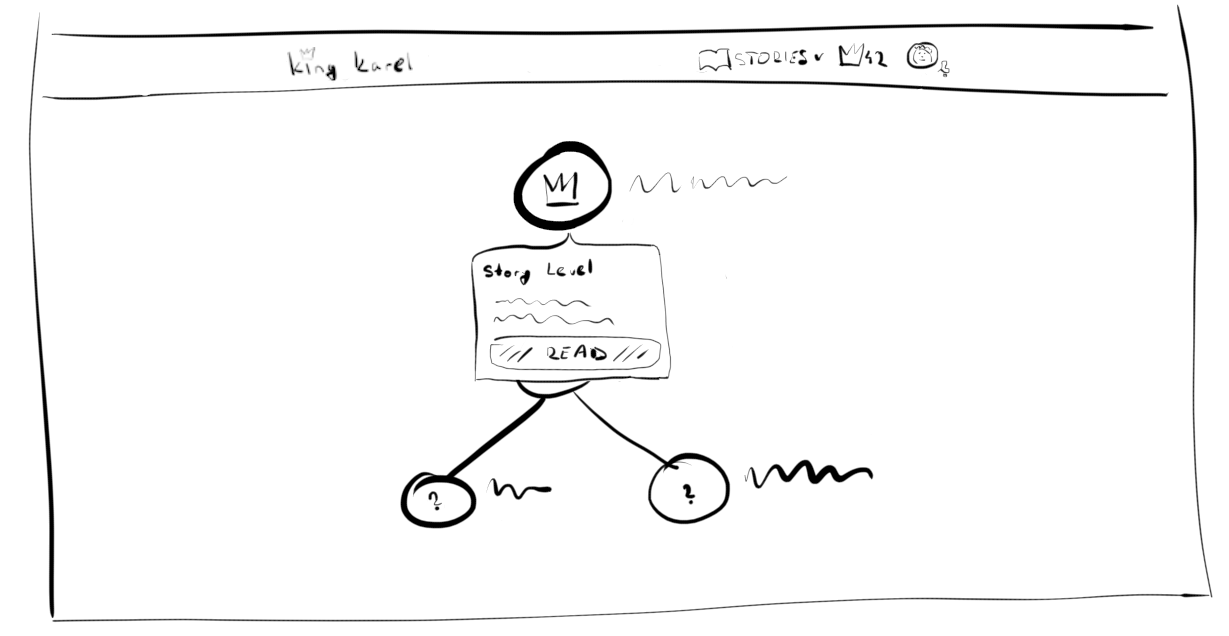
\includegraphics[width=1\linewidth]{assets/design/ui/wir_story.png}
    \caption{Learning and Storytelling Missions Wireframe}
    \label{fig:design:wir:story-learning}
\end{figure}

\subsection{Game Mission Screen}

The main part of the prototype of the developed game is on the screen \ref{fig:design:wir:game-mission}.
It contains both a top menu that includes buttons to jump to the main screen, stories, statistics, and a profile.

The screen contains a panel with command blocks on the left.
These are arranged below each other and possibly nested inside each other.
To the right of this is a palette of commands that can be used for a given mission.

Below these panels, there is no panel at the bottom with buttons to save and stop the game.

In the right part of the screen, there is a grid display that represents the game's current state.
The grid can display walkable lungs or non-walkable squares that form walls or other types of obstacles.
The grid also shows a doll that marks the robot, Karel.
That is the character the player is playing as.

\begin{figure}
    \centering
    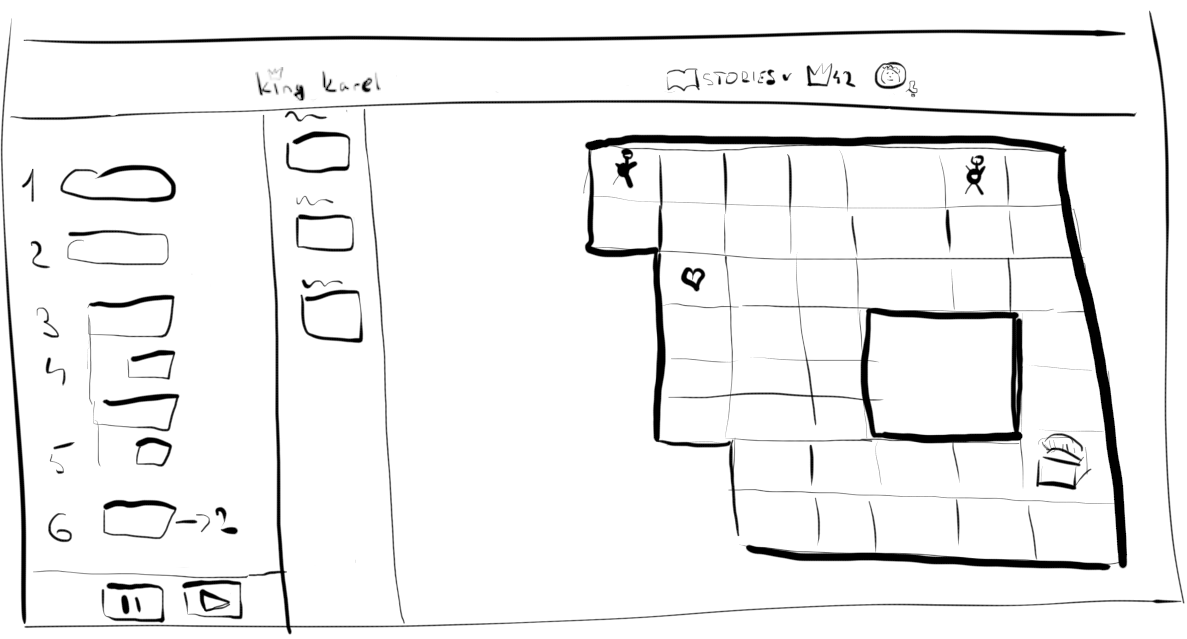
\includegraphics[width=1\linewidth]{assets/design/ui/wir_game_mission.png}
    \caption{Game Mission Wireframe}
    \label{fig:design:wir:game-mission}
\end{figure}

\subsection{Game Dialog}

At the end of the game, whether successful or not, a \ref{fig:design:wir:game-dialog} dialog window will appear with a status message.
This dialog reports whether the game ended with an error or successfully.
In addition, the dialog contains a caption.
The optional size and speed bonus attributes are displayed if the status is successful.

\begin{figure}
    \centering
    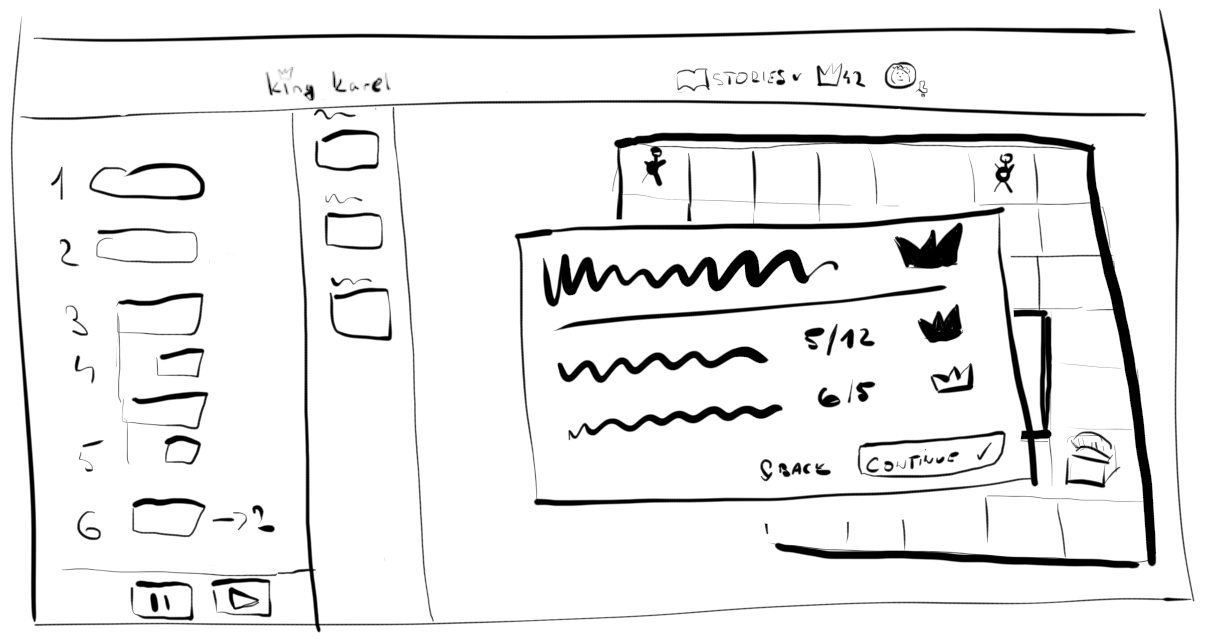
\includegraphics[width=1\linewidth]{assets/design/ui/wir_game_dialog.png}
    \caption{Game Mission Dialog Wireframe}
    \label{fig:design:wir:game-dialog}
\end{figure}

\subsection{Statistics Screen}

The statistics screen \ref{fig:design:wir:statistics} shows the status of success of game missions and values of the optional size and speed attributes.
It displays it in the tabular form separately according to yourself and other players.
The statistics are divided according to the game mission.

\begin{figure}
    \centering
    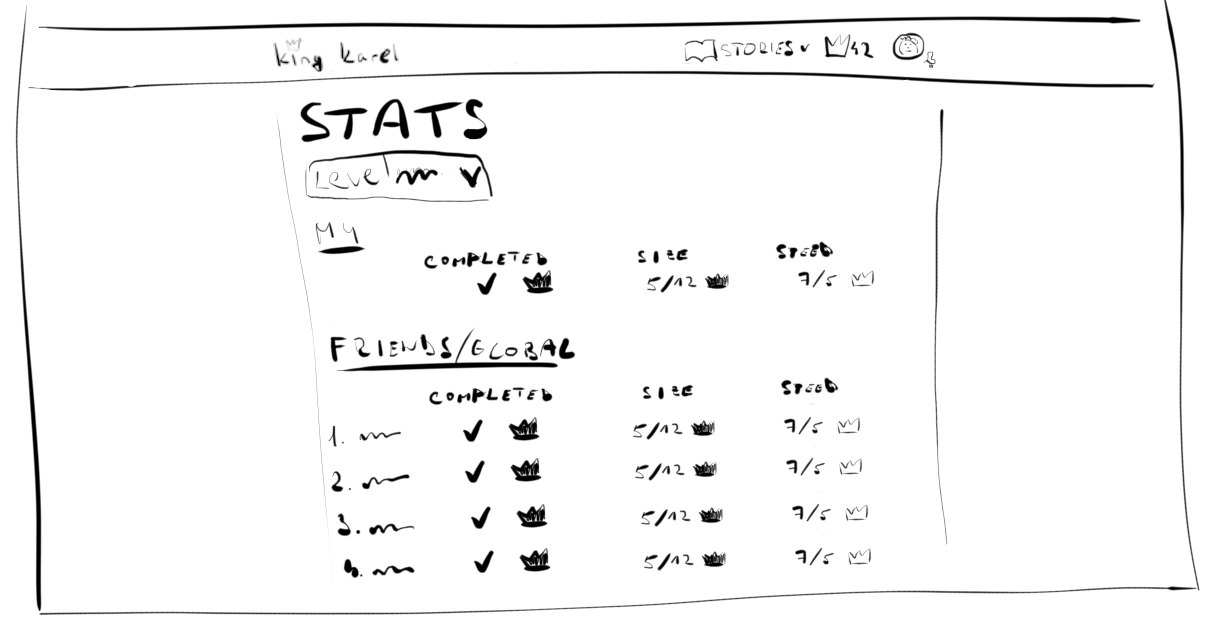
\includegraphics[width=1\linewidth]{assets/design/ui/wir_stats.png}
    \caption{Statistics Wireframe}
    \label{fig:design:wir:statistics}
\end{figure}


\chapter{Implementation}
\label{chapter:implementation}

This chapter describes exciting parts of the implementation or possible problems encountered during the implementation.
It describes the client application, server application, database, and user interface design implementation.

\section{Client Application}

In the design chapter \ref{chapter:design}, the following technologies were selected for the client application implementation.
According to the design, the implemented application must support web and Windows and other desktop platforms, respectively.
It must also be easily extensible to mobile devices.
Therefore, the Flutter framework was chosen, enabling cross-platform development on web, desktop, and mobile platforms.
The Bloc library was chosen for the state management app state, which, thanks to its asynchronous approach, provides a robust implementation and allows easy expansion or modification.

\subsection{Used Technologies}

The Flutter framework in version 2.10.5 was used on its stable channel.
This version uses the Dart programming in version 2.16.2.
The package \mintinline{text}|flutter_bloc| in version 8.0.1 was used in the presentation layer for providing the Bloc library.
This package provides the basic implementation of the Bloc library and supporting widgets and other things for use with the Flutter framework.

The package \mintinline{text}|get_it| in version 7.2.0 was used for dependency injection in the presentation layer.
This package allows registering specific class implementations to their interfaces.
Registered classes are then located from anywhere in the code.

The data layer uses the package \mintinline{text}|http| in version 0.13.4 for the HTTP communication.
This package provides an interface for sending HTTP methods POST, GET, PUT, DELETE, etc.

The business layer uses package \mintinline{text}| shared_preferences| in version 2.0.13 to store the token.
This package stores data in the appropriate place based on the platform.

\subsection{Command Blocs Rendering}

Command blocks are one of the most critical components of the implemented game and their implementation, and the whole development process was fascinating.
These are used for visual programming of individual game missions.
Before describing the development of this feature, there is a little reminder of what command blocks are and how they should behave.
Command blocks are used to program a game mission.
Blocks are visual components that can be grabbed and moved within the left panel of the game mission screen.
An example of command blocks is in the figure \ref{fig:commandblocks}.
Blocks are part of the command block list, and if a player tries to drop a block outside that list, the command is deleted.
The player can use command blocks that are available in the command block palette.
Command blocks can be dragged to the command block list from this palette.

\begin{figure}
    \centering
    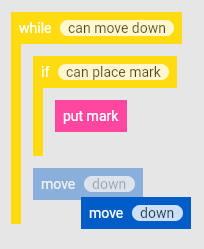
\includegraphics[width=0.4\linewidth]{assets/implementation/commandblocks.png}
    \caption{Command Blocks}
    \label{fig:commandblocks}
\end{figure}

Command blocks use widgets for their implementation.
The initial idea for the implementation was to use one of the already existing widgets of the Flutter framework.
Flutter contains several widgets that could handle similar functionality, so several options have been tried.

One of the ways to implement this could be \mintinline{text}|ReorderableListView| widget from the Flutter Material library.
According to \cite{a2022_material}, this widget works like a regular widget that positions its children in a column, provides scrolling, and allows to drag items within the list.
This widget provides different drag-and-drop behavior based on whether it's used on a mobile device where the player uses a finger to drag or on a web where the player uses a mouse to drag elements.
All elements of the list must have a unique key.
The \mintinline{text}|ReorderableListView| widget would work well if it did not need to be able to nest command blocks.
However, this widget does not support element nesting, and a similar solution using this widget failed.
In addition, the elements in this widget only drag inside their container, which is also not required.
The elements should be possible to drag in all directions and across different containers or drag elements from the command block palette.

Another option would be to use the \mintinline{text}|Draggable| and \mintinline{text}|DraggableTarget| widgets.
These widgets, according to \cite{a2022_material}, work in their interplay.
Widget \mintinline{text}|Draggable| defines the data that the widget should transmit.
This widget also has three children that differentiate what the widget should look like, what the widget should look like when dragged, and how the area behind the widget should look.
The second widget, widget \mintinline{text}|DraggableTarget|, is used to determine where \mintinline{text}|Draggable| widget can be dragged.
It defines several functions according to which the widget determines whether the dragged widget should be accepted or what should happen if dropped.
It also defines a builder that determines how the widget should appear based on whether or not any data has been dragged to it.
This approach sounded very promising at first; however, it turned out that it would be complicated to use these widgets to make a dynamic implementation within the scope of command block requirements.
One problem was that if a new command block was added to the end of the command block list, how to create a new slot for the next block.
It would also be challenging to implement blocks reordering.
Additional empty \mintinline{text}|DraggableTarget| widgets would have to be added to all the used \mintinline{text}|DraggableTarget| widgets to check if the player moves the block to one of the locations between blocks.
After moving the block, a recalculation would have to follow, and a similar situation would be repeated.

Command blocks must be rendered declaratively because widgets in the Flutter framework are rendered declaratively.
Because the position of all blocks would have to be complicatedly mapped to the state, the second proposed option could not be implemented.
Because of this, a custom solution was created.
The solution contains two essential elements, containers, and blocks.
A container is a widget that will accept blocks.
And blocks are widgets that represent commands.
Some blocks also contain a nested container to which the exact definition applies.
In addition, this container and block structure is defined by a state, which is represented as a command tree structure.
These commands are of two basic abstract types and can be group or single commands.
Each command has its class that extends one of these abstract classes.
A special case is the root command class, which is used as the root of the tree structure.
That makes a declarative rendering of the structure.
It uses its widget \mintinline{text}|CommandItem|, to which an instance of the command is passed as an argument, and according to its abstract type, other \mintinline{text}|CommandItem| widgets are recursively added to the widget tree.
These \mintinline{text}|CommandItem| widgets then add the widget \mintinline{text}|CommandBlock| to the structure, which solves the visual rendering of the command block, i.e., displays the colored rectangle of the command.
The entire display of list command blocks takes place in the \mintinline{text}|CommandsView| widget.

The moving command blocks feature is missing to complete the required functions.
For \mintinline{text}|CommandBlock| widget to drag, the player must hold and move it.
As the player drags the block, the \textquote*{shadow} (as can be seen in the figure \ref{fig:commandblocks}) of the original block must remain beneath it, which moves to the location where the block could be placed as it drags.
It must also be determined in which specific container this block is to be placed.
Whether in the main or in one of the nested, which belong to the commands that have nested blocks.
If the block is moved outside of any container, the \textquote*{shadow} will soften, indicating that it will be removed if the player releases the block.
Conversely, the block must also be able to be moved and copied from the command palette.
All these operations continuously update the state of the command tree structure.
The blocks themselves are not physically moved.
The state according to which the widgets are redrawn changes.
The \mintinline{text}|Key| keys are used to ensure that the framework does not redraw blocks that do not change or that the algorithm knows which widget to move.
Keys are, according to \cite{a2022_material}, unique widget identifiers.
The key for the \mintinline{text}|CommandItem| widget is an \mintinline{text}|ObjectKey| key using the object of the respective command, i.e., its hash.

The move is processed in the \mintinline{text}|CommandsView| widget.
All blocks and containers are registered in this widget so that this widget can subsequently browse them.
To start a move event, the \mintinline{text}|CommandBlock| widget (which draws a visual rectangle) uses the \mintinline{text}| Listener| widget, which according to \cite{a2022_material} provides an interface to basic pointer events.
Specifically, the \mintinline{text}|PointerDownEvent| event is captured.
This event is passed to the \mintinline{text}|CommandsView| widget, which starts processing the move.
It also starts listening to other events using the Flutter class \mintinline{text}|PanGestureRecognizer|.
It provides an interface for capturing update and end events.
Widget \mintinline{text}|CommandsView| uses the \mintinline {text}|Stack| widget, which allows to display widgets on top of each other.
It will display a special proxy widget at the top of this stack.
Visually, this widget is the original widget being dragged.
However, as described above, the original widget remains in place as a \textquote*{shadow.}
This added proxy widget is the one that is being dragged.

For each update event, the position of the proxy widget must be updated by the delta difference of the event.
Subsequently, a lookup is performed to find the nearest container in which the event position is located, i.e., the player's pointer.
If no container is found, the dragged command bloc is marked as suitable for deletion.
If found, the block closest to the dragged block is also found.
That determines the position to which the block's \textquote*{shadow} should move.
The state is updated, and Flutter declaratively redraws the command blocks, so the \textquote*{shadow} visually moves to the correct position.

Iteration through all registered containers is used for the lookup of the nearest container.
The current container's \mintinline{text}|RenderObject| or \ mintinline{text}|RenderBox|, respectively, is requested using \ mintinline{dart}|final containerRender = container.context.findRenderObject () and RenderBox;|.
Then, as can be seen in the code \ref{listing:closest-container}, the position of the container is compared with the cursor position, and then, if the container is not part of a block (that is if the container is not a block subcommand), the nearest such container is found.
A similar algorithm finds the nearest block below.

\begin{listing}
    \caption{Closest Container Lookup}
    \label{listing:closest-container}
    \begin{minted}{dart}
if (containerRender.size.contains(
    position 
        - containerRender.localToGlobal(Offset.zero) 
        + const Offset(2, 2)
)) {
    // But it is not subtree of original item.
    if (!container._isChildOfItem(_dragging!)) {
    // Find closest one.
    if (container.index.length > maxIndexes) {
        maxIndexes = container.index.length;
        closestContainer = container;
    }
    }
}
    \end{minted}
\end{listing}

Some blocks may have conditions or directions.
These are also rendered by the \mintinline{text}|CommandBlock| widget if the command has a choice of condition or direction.
An overlay must be created when the mouse is moved over for a player to be able to select a condition or direction in such a block.
The options are displayed in the respective overlay, and after selecting the option, the command state is adjusted.

\subsection{Overlays}

The custom widget \mintinline{text}{OverlayButton} is used to implement overlays.
This widget is used to select conditions and directions for command blocks in the game mission and for some submenu buttons in the menu.

\begin{figure}
    \centering
    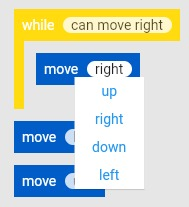
\includegraphics[width=0.4\linewidth]{assets/implementation/overlay.jpeg}
    \caption{Overlay}
    \label{fig:overlay}
\end{figure}

Overlays display content above the standard widget tree.
Such logic could be created using a custom implementation using the \mintinline{text}|Stack| widget.
Implementing it this way for all applications can be annoying and error-prone.
Flutter provides the \mintinline{text}|Overlay| widget, which implements exactly this functionality.
This can be used to display input suggestions, tooltips, or anything that needs to float above the screen.
According to \cite{a2022_material}, \mintinline{text}|Overlay| is \textquote{A stack of entries that can be managed independently.}
\mintinline{text}|Overlay|, therefore, maintains its \mintinline{text}|Stack| and manages widgets that are added to it.
This widget can be created directly, or it can be used already pre-created one using the \mintinline{text}|Navigator|.
An example of an overlay for a command block can be seen in the figure \ref{fig:overlay}.

To create an overlay, the \mintinline{text}|insert()| method needs to be called on the mentioned \mintinline{text}|Overlay| created by \mintinline{text}|Navigator|.
\mintinline{text}|OverlayEntry| is used as an argument for this method.
According to \cite{a2022_material}, \mintinline{text}|OverlayEntry| is the object that \mintinline{text}|Overlay| use to represent its items.

In addition, the custom \mintinline{text}|OverlayButton| widget, which is used for overlays in the game mission, menu, etc., detects if the overlay overflows the screen to the right or left and adjusts it to be at its edge instead.
Because in some cases, it is necessary to ensure that the overlay moves with the widget that triggered it.
For example, when scrolling, it is necessary to synchronize the position on the screen.
It can also be used only to synchronize the position, whether it will change later.
That can be implemented manually, but Flutter has ready functionality for this.
Flutter provides the ability to create a \mintinline{text}|LayerLink| object that allows linking a follower to a target \cite{a2022_material}.
\mintinline{text}|OverlayEntry| can use the \mintinline{text}|CompositedTransformFollower| widget to set the follower and \mintinline{text}|CompositedTransformTarget| to set the target.
The follower will automatically follow the position of the target.
\mintinline{text}|OverlayButton| detects enter and end events on the widget and displays the overlay accordingly.

\subsection{Networking}

The \mintinline{text}|http| package is used for networking.
The package is used to communicate with the Web API server.
From there, JSON encoded data are fetched.
Fetched data are decoded into \mintinline{dart}{Map<String, dynamic>} data and are further processed to create entities.
Most of the entities has a factory constructor \mintinline{dart}|.fromJson(Map<String, dynamic> json)|.
These constructors parse the typed JSON and create entities from it.
A simple example of the user entity can be seen in the code \ref{listing:fromjson}.

\begin{listing}
    \caption{From-Json Factory Constructor}
    \label{listing:fromjson}
    \begin{minted}{dart}
factory User.fromJson(Map<String, dynamic> json) {
    return User(
        id: json['id'],
        name: json['name'],
        username: json['username'],
        email: json['email'],
        description: json['description'],
    );
}
    \end{minted}
\end{listing}

Data are usually simple to parse.
There are some compelling cases in which the parsing is more complicated.
After loading a game mission, a \mintinline{text}|GameMission| entity is created.
This entity contains all its properties as simple data types.
But it contains the \mintinline{text}|commands| and \mintinline{text}|commandsInitial| properties that contains a string with a encoded JSON structure.
This structure must be further decoded and processed.
That is done by the \mintinline{text}|GameMission|'s \mintinline{text}|parseGame()| method.
This method decodes the command's properties to the JSON map and recursively creates a commands tree using the factory constructor of the \mintinline{text}|RootCommand|.
This constructor parses its data which are recursively parsed to the specific command classes.
This process, therefore, elegantly creates a command tree structure.

\subsection{Router and Navigation}

Flutter initially used an imperative approach to routing and navigation.
According to \cite{ryan_2020_navigator}, this was problematic, and it was challenging to push or pop several screens or otherwise change the state of the screen stack.
A new Navigator 2.0 API has been added to Flutter, allowing control of the navigator declaratively.
A schema of Navigator 2.0 can be seen in the figure \ref{fig:navigator}.
According to \cite{kietay_2021_navigator}, the imperative approach can get the application into trouble because it does not separate app logic from the UI logic.
UI logic is separated from app logic using a declarative approach.
UI logic displays screens according to data, respectively depending on the application's state.
And app logic retrieves data and changes the state of the application.

\begin{figure}
    \centering
    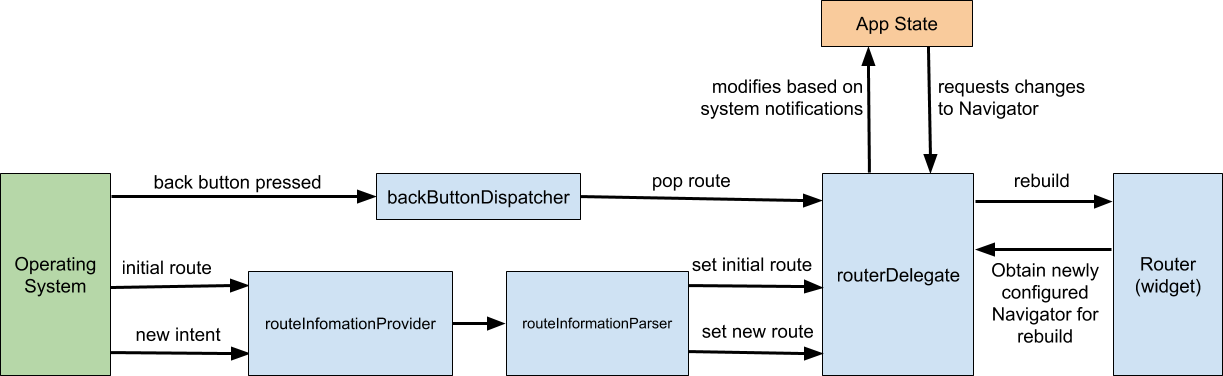
\includegraphics[width=1\linewidth]{assets/implementation/navigator.png}
    \caption{Navigator 2.0 \cite{ryan_2020_navigator}}
    \label{fig:navigator}
\end{figure}

According to \cite{kietay_2021_navigator}, Navigator 2.0 needs to do three things.
Convert app state to navigator state (build method).
Convert app state to Abstract Data Type (ADT) and further to the path.
And convert the path to the ADT and then to the app state.
According to \cite{ryan_2020_navigator}, two new classes are used for this.
The \mintinline{text}|RouteInformationParser| class, which uses the \mintinline{text}|parseInformationRouter| to convert the path to the ADT and uses the \mintinline{text}|restoreRouteInformation| method to convert the ADT to the path.
And the \mintinline{text}|RouterDelegate| class, which uses the \mintinline{text}|setNewRoutePath| to convert the ADT to app state and the \mintinline{text}|currentConfiguration| method to convert app state to the ADT.

Several screens have been created for the implemented game, each of which must have an appropriate representation using a path, navigation state, and app state.
According to the text above, the Bloc library is used as the app state, which represents the app state.
Of course, this state is only in the context of routing.
It contains several states (and therefore screens) that can extend interfaces.
Interface \mintinline{text}|RequiresAuthentication| is used to indicate those states that require the user to be able to access them only when logged in.
This Bloc, therefore, communicates with the Bloc that manages the authentication.
Before Bloc invokes a state redirecting to a given screen, it checks that the user is signed in if the future state implements this interface.
It also contains the \mintinline{text}|ForbiddenAfterAuthentication| interface, which works very similarly to the former.
If the user tries to get to the screen, they will be redirected to the sign-in screen instead.
The difference is that Bloc will not emit those states that redirect to that screen if the user is signed in.
That is used for sign-in and sign-up screens that are only available to anonymous users.
If the user still tries to get to the screen, they will be redirected to the home screen.
The scheme of individual states and their attributes can be seen in the figure \ref{fig:routing}.

\begin{figure}
    \centering
    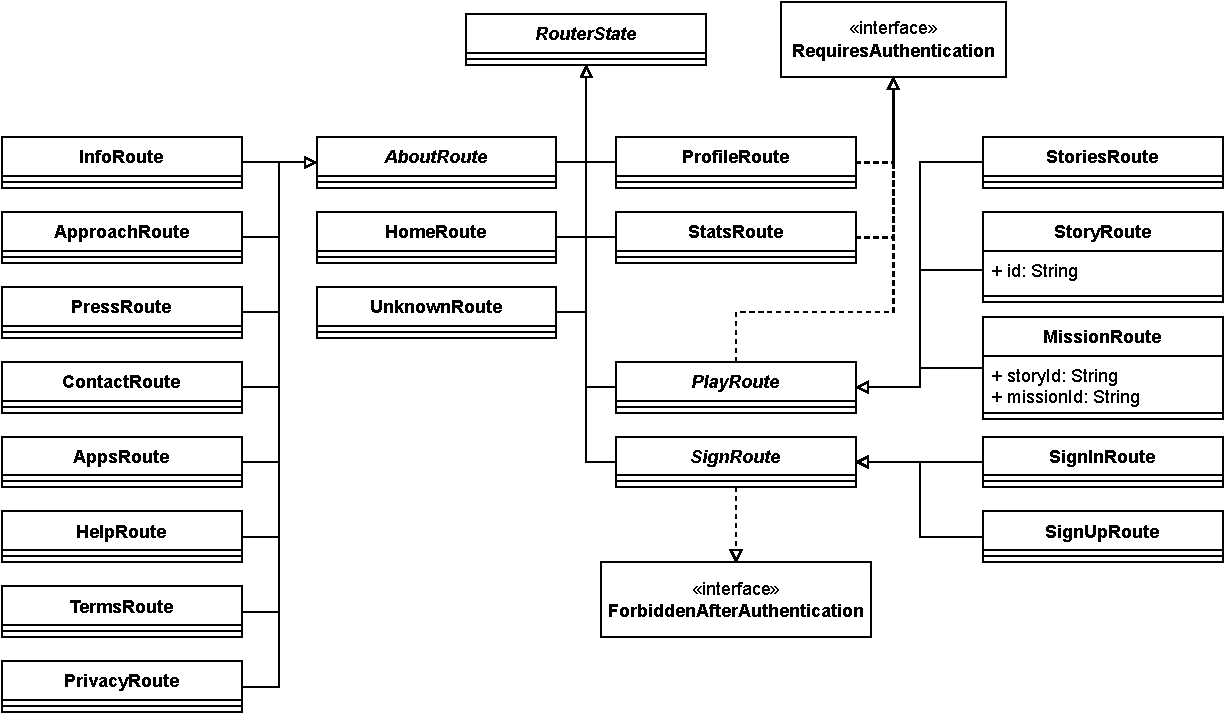
\includegraphics[width=1\linewidth]{assets/implementation/routing.pdf}
    \caption{Routing}
    \label{fig:routing}
\end{figure}

\subsection{Game Processing}

At the beginning of this section, command blocks were described as one of the critical components of the implemented game.
Game missions consist of two critical parts.
One is the part with the visual programming, wherewith the help of command blocks, the player moves the commands to the correct order so that the robot performs the correct sequence of steps and fulfills the mission goal.
The second part is the game processing.
That includes both game grid implementation, visual representation of the game state, and processing of visual programming (command blocks).

\begin{figure}
    \centering
    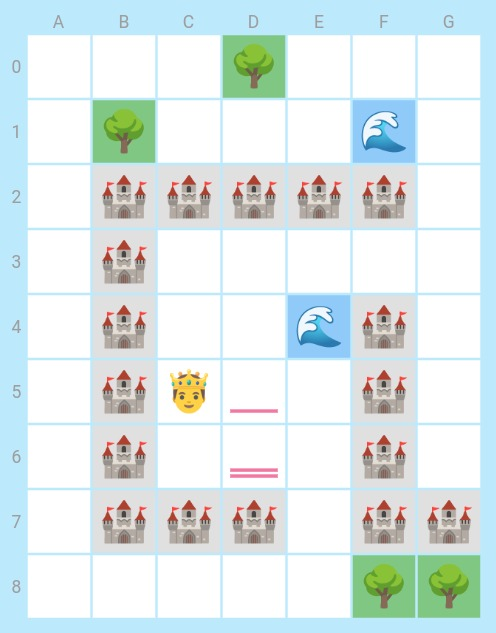
\includegraphics[width=0.5\linewidth]{assets/implementation/gamegrid.jpeg}
    \caption{Game Grid}
    \label{fig:gamegrid}
\end{figure}

The game grid is implemented as a grid of cells.
It can be seen in the figure \ref{fig:gamegrid}.
These, like command blocks, use widgets to render.
These widgets are rendered into several types according to the type of each cell.
A walkable cell is rendered as an empty cell that a robot can walk on.
This cell can also have several marks.
These appear as horizontal plates.

Then several types of non-walkable cells are implemented.
These are walls, forests, and water.
The wall has a gray coloration and represents, for example, the castle walls.
The forest has a green coloration and represents an impenetrable forest.
Water has a blue tint and represents water.
The robot must not get out of the walkable cells.
If a player tries to step outside the walkable cell or the grid, the game will allow him to see his mistake visually in the first step.
After this step, however, the game opens a failed game dialog, where it reports its error.
That can be seen in the figure \ref{fig:gamedialog}.
Coordinates with numbers for the vertical axis and letters for the horizontal axis are displayed around the grid.
The coordinates are also displayed when you hover a cell to make navigation easier when thinking about how to complete the game.

\begin{figure}
    \centering
    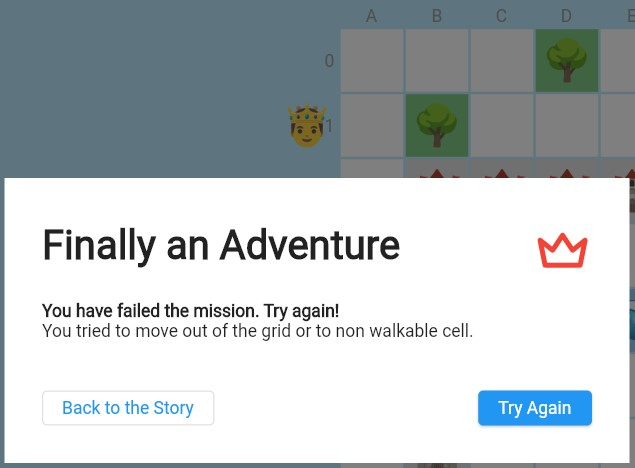
\includegraphics[width=0.7\linewidth]{assets/implementation/gamedialog.jpeg}
    \caption{Game Dialog}
    \label{fig:gamedialog}
\end{figure}

In order for the player to know clearly where they are in each step, the robot is marked on the grid with a figure with a crown.
As the game progresses, this character moves around the grid to perform the tasks assigned by the visual programming.
At the same time, the currently executed command block is indicated by an arrow.
In this way, the player knows which command is currently being executed and which is responsible for potential unplanned behavior.

After clicking the play button, the current command blocks are saved, and an event to play the game is added with those commands.
The game itself is processed in the \mintinline{text}|processGame()| method in class \mintinline{text}|GameService|, or rather in its implementation class \mintinline{text}|GameServiceImpl|.
This method receives as an argument an entity with all the game data.
The algorithm thus has access to all the necessary data.
The output of this method is the queue of the \mintinline{text}|ProcessGameResult| object.
This object contains the object with the game and the index of the currently processed command.
If an error occurred in the given step, the type of an error is also included. 
The algorithm first determines if the commands are valid.
That is checked by recursively passing commands using their \mintinline{text}|isValid()| method.
If the commands are valid, the commands begin to be processed recursively.
The algorithm gradually calls group and single command processing methods according to the given command type.

For the single command type, the process is trivial.
The algorithm creates a clone of the game object modified by the given command effect.
Then it is added to the queue.
If an error occurs during processing, an error is also added to it.

For the group command type, the command \mintinline{text}|if| is processed separately from the \mintinline{text}|while| command.
Both commands first add a state to the queue, pointing to the index of their command block.
Command \mintinline{text}|if| then it checks the condition and, if it is met, it calls the method to process the nested commands.
Command \mintinline{text}|while| works similarly, but the condition is checked in a while loop.
During this pass, the \mintinline{text}|speed| argument is counted, which indicates the number of executed commands of the given command, i.e., the method call for solving a group or single command.

The \mintinline{text}|size| argument is also calculated at the beginning of processing, which indicates the number of blocks used.
The \mintinline{text}|countSize()| method is invoked over the root command object.
After the recursive processing is completed, the last state is added to the queue with the game modified by filled \mintinline{text}|size| and \mintinline{text}|speed| attributes, and the \mintinline{text}|completed| attribute, which indicates whether the game was completed.
This is detected by calling the \mintinline{text}|isCompleted()| method on the game object.

\section{Server Application}

The design chapter \ref{chapter:design} selected the ASP.NET Web API in version 6.0.102 with C\# and the Entity Framework in version 6.0.3 tool.

All services and repositories interfaces implementations are registered in the dependency injection tool provided by the ASP.NET.
The dependency injection tool allows automatic injection into constructors, thus abstracting the process of creating most objects.
This is a kind of magic compared to other languages and technologies, but it works well.
Registration is done in the \mintinline{text}|Startup| class that in the \mintinline{text}|ConfigureServices| method uses \mintinline{text}|IServiceCollection| to register.
Controllers are also registered in a similar way using the \mintinline{csharp}|services.AddControllers()| method that an automatic registration of all controllers.
Services and repositories are registered using \mintinline{csharp}|services.AddScopped<InterfaceType, ImplementationType>()|.

Setting up configurations for the game is also made in the \mintinline{text}|ConfigureServices|.
For configuration a combination of standard public file \mintinline{text}|appsettings.json| and a secret file \mintinline{text}|secrets.json| can be used.
The structure of the game's configuration can be seen in the code \ref{listing:serverconfig}.
The \mintinline{text}|DatabaseUrl| and \mintinline{text}|JwtSecret| should be stored in a secured file.

\begin{listing}
    \caption{Server Configuration}
    \label{listing:serverconfig}
    \begin{minted}{json}
{
    "AppSettings": {
        "DatabaseUrl": "<db url>",
        "JwtSecret": "<token>",
        "CorsOrigins": [
            "http://localhost:8080"
        ]
    }
}
    \end{minted}
\end{listing}

The primary purpose of the server application is to provide a Web API that handles storing and fetching the game's data.
It uses controllers to handle incoming HTTP requests.
Controllers use injected services that handle all logic.
Services usually use injected repositories that communicate with the database using the Language-Integrated Query (LINQ) to Entities.
LINQ to Entities can be used on the \mintinline{text}|DbSet| properties of the \mintinline{text}|DbContext| object.
An example of such usage in LINQ method syntax can be seen in the code \ref{listing:linq} that shows a fetch of missions for a specific story.

\begin{listing}
    \caption{LINQ to Entities}
    \label{listing:linq}
    \begin{minted}{csharp}
var missions = _dbContext.Stories
    .Include(s => s.Missions)
    .FirstOrDefault(s => s.Url == storyUrl)
    ?.Missions;
    \end{minted}
\end{listing}

\subsection{Saving the Game Progress}

To save the game progress the HTTP PUT method on \linebreak\mintinline{text}|{storyUrl}/{missionUrl}| resource must be called.
It should contain \linebreak\mintinline{text}|GameProgressDto| data, which includes commands as an encoded JSON in a string, speed and size attributes as an int, and the completed attribute as a bool.

Inside of the controller, the \mintinline{text}|StoryService| is called with the \linebreak\mintinline{text}|SaveGameProgress| method.
Inside the service, an eponymous method is called on the \mintinline{text}|StoryRepository|.
Inside the repository, if game progress existed before, it is fetched.
If there is already an existing record, its data get updated.
Otherwise, a new \mintinline{text}|GameProgress| object must be created.
An important note is that the created object must contain a reference to the user and game entities.
Therefore they must be fetched and used.

\subsection{Fetching Story's Missions}

The \mintinline{text}|StoryRepository| repository also contains the \mintinline{text}|GetMissions| method.
That is used to fetch missions of all types.
Because the game mission can have an associated \mintinline{text}|GameProgress| record for the specified user, a join has to be made.
LINQ contains two joins.
The \mintinline{text}|Join()| method corresponds to the SQL's inner join.
And the \mintinline{text}|GroupJoin()| method that corresponds to the SQL's left outer join.
For this purpose, the \mintinline{text}|GroupJoin()| method was used.
The code of the left outer join can be seen in the code \ref{listing:groupjoin}.
Note that \mintinline{text}|missions| contains all missions of the selected story.
It also uses the \mintinline{text}|resultSelector| that merges the joined data and converts the entity from the entity to do a more suitable DTO.

\begin{listing}
    \caption{GroupJoin to Fetch Story's Missions}
    \label{listing:groupjoin}
    \begin{minted}{csharp}
var queryData = missions.OrderBy(m => m.Order)
    .GroupJoin(
        _dbContext.GameProgresses.Where(
            progress => progress.User.Id == userId
        ),
        m => m.Id,
        gp => gp.Game.Id,
        (mission, progresses) => GetMissionDtoFromGroupJoin(
            mission, progresses.SingleOrDefault()
        )
    ).ToList();
    \end{minted}
\end{listing}

DTOs cannot return different data based on inheritance.
For this purpose, the \mintinline{text}|GetMissionDtoFromGroupJoin()| method returns the \mintinline{text}|MissionsListDto|, which has two subtrees: either inside a game property or a learning property; the other is null.
This way, inherited data can be returned in response to the client from the controller.
A better solution was not found.

\subsection{Tokens}

The tokens were discussed in the \ref{design:server:tokens} chapter.
\mintinline{text}|JwtService| service uses the \mintinline{text}|Microsoft.AspNetCore.Authentication.JwtBearer| library in version 6.0.3 for token generation and validation.

For the generation, it uses the user's id as an id claim, expiration is set to seven days, and it is signed using the \mintinline{text}|HmacSha256Signature| algorithm.
Mentioned and other data create the \mintinline{text}|SecurityTokenDescriptor| and the \mintinline{text}|JwtSecurityTokenHandler| then creates the token from it.

Validation of the token uses \mintinline{text}|ValidateToken()| from the \linebreak\mintinline{text}|JwtSecurityTokenHandler| object.

Clients must add JWT to the authorization header like \linebreak\mintinline{text}|Authorization: Bearer <jwt-token>|.
A custom authentication scheme \linebreak\mintinline{text}|KingKarelAuthHandler| is used to validate the token.
The handler checks the presence of the authorization header and whether it starts with the \textquote*{Bearer} string.
The handler then uses the \mintinline{text}|JwtService| that tries to validate the token.
If the token is valid, the id claim is fetched from the token and added as the identity claim to the \mintinline{text}|AuthenticationTicket|.
Controllers then can use these claims by accessing \mintinline{text}|User.Claims|.

\subsection{Passwords}

Passwords are hashed using the \mintinline{text}|BCrypt.Net-Next| library in version 4.0.3.
The library provides the \mintinline{text}|BCrypt| object that has a method \mintinline{text}|HashPassword()| that hashes a password with a generated salt.
It also provides the \mintinline{text}|Verify()| method that requires a password and a hashed password arguments. 
Only hashed passwords are stored in the database.

\begin{figure}
    \centering
    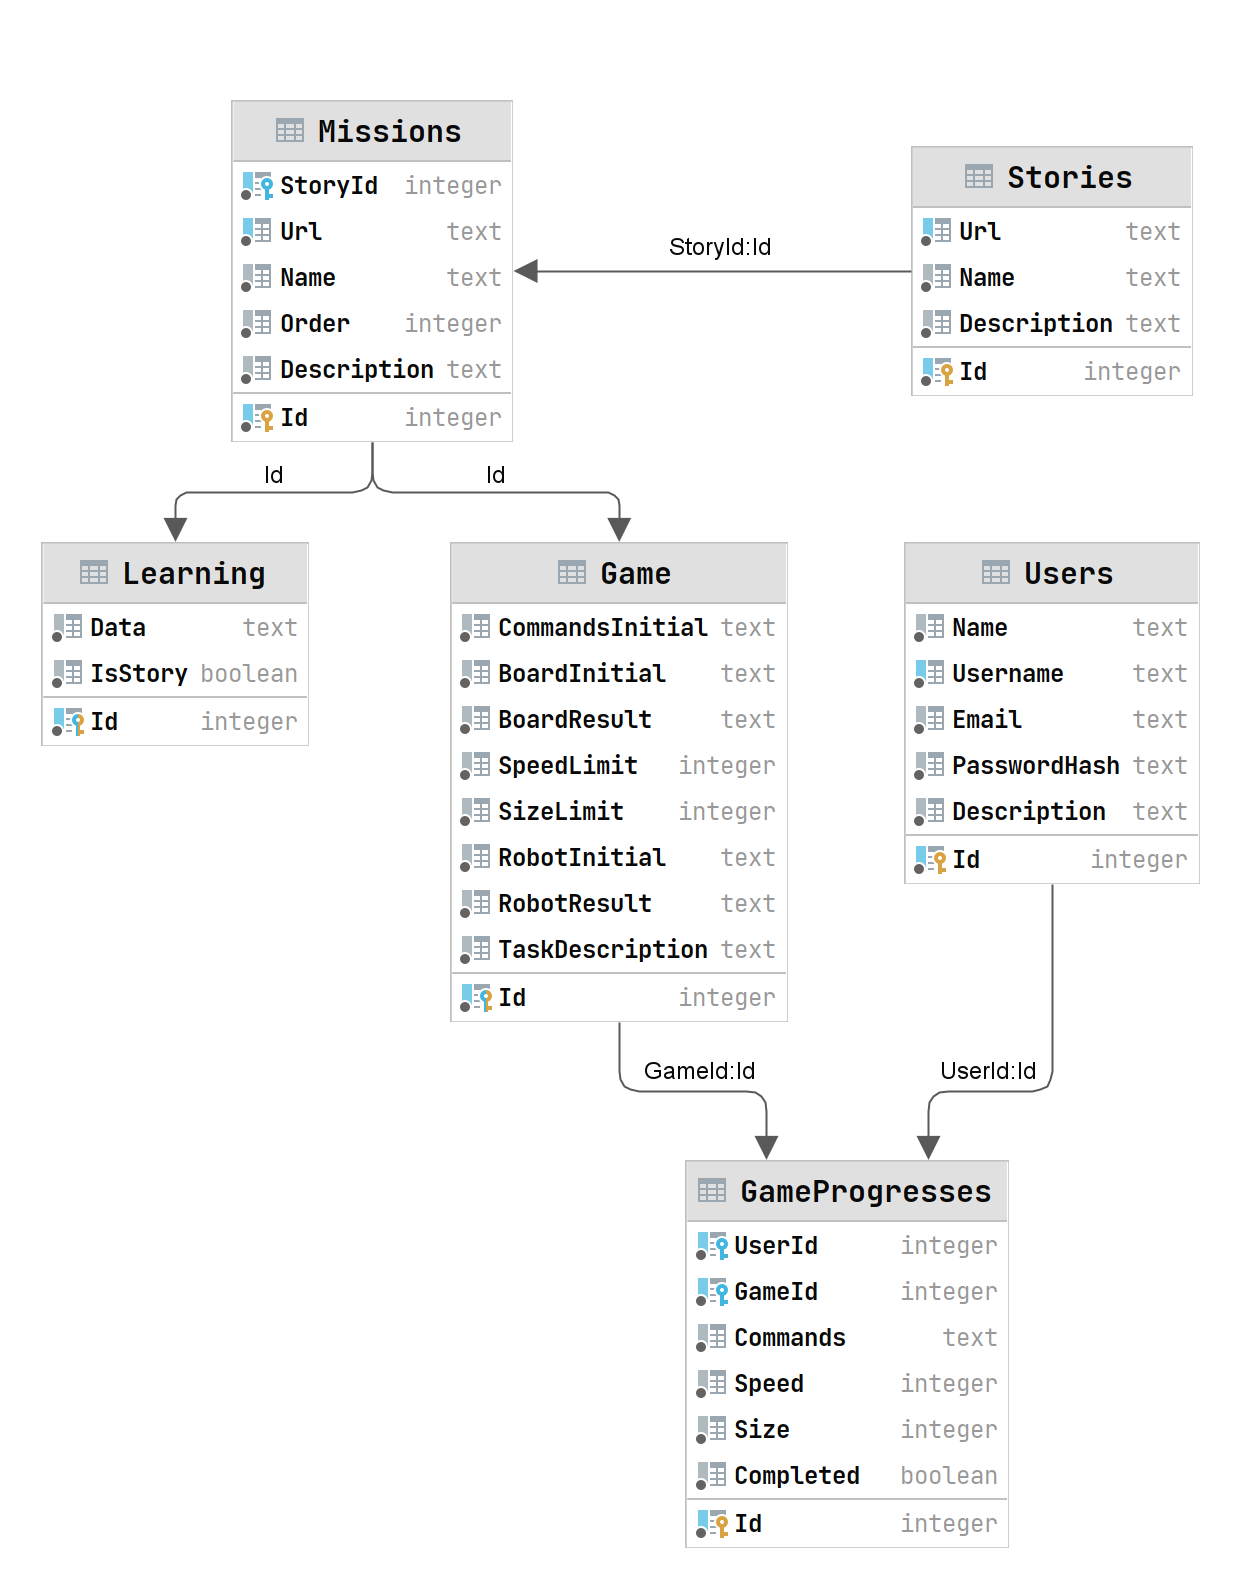
\includegraphics[width=1\linewidth]{assets/implementation/erdiagram.png}
    \caption{Relational Schema}
    \label{fig:impementation:relationalschema}
\end{figure}

\begin{listing}
    \caption{Entity Framework Migration Tools}
    \label{listing:migration}
    \begin{minted}{shell}
# installation
dotnet tool install --global dotnet-ef

# create a migration
cd KingKarel
dotnet ef migrations add "Name of migration"

# update the database
dotnet ef database update
    \end{minted}
\end{listing}

\section{Database}

According to the~design chapter~\ref{chapter:design}, PostgreSQL was used as a~database for the~game.
For local development, a~docker container with the~database is set up.
The~docker-compose file is located in the~server application project.

In the~chapter~\ref{design:conceptual} a~conceptual schema is described.
According to that schema, a~relational schema was created.
The~relational schema can be seen in the~figure~\ref{fig:impementation:relationalschema}.
The~strucute of relational schema is similar to the~structure of the~conceptual schema.
For unique identifiers integer data types are used.
For other attributes an~integer, a~string, or a~boolean data types are used.
Inside some of the~string attributes an~encoded JSONs are stored.

\subsection{Migrations}

Migrations manage the~database from the~server application.
Entity framework tools support the~creation and updates of migrations.
That is useful, especially when the~database schema is created using the~ORM from the~code.
Each migration creates a~file with the~\mintinline{text}|Up()| and \mintinline{text}|Down()| methods.
These methods allow migration tools to apply and undo a~migration.
Migration files are generated to \mintinline{text}|KingKarel/Migrations| directory.
Useful migration tool's commands can be seen in the~code~\ref{listing:migration}.

\section{User Inteface}

In this chapter, implemented user interface screens will be presented and discussed.
They are based on wireframes discussed in chapter \ref{design:ui}.

\subsection{Game Mission Screen}

In the figure \ref{fig:implementation:ui:game-mission} there is a game mission screen.
It consists of two parts.
The left part contains a visual programming tool that includes commands blocks, its palette, and button used to play, save, and reset the game, and a show or hide description button.
The right part contains a game grid that dynamically changes while the game progresses.

\begin{figure}
    \centering
    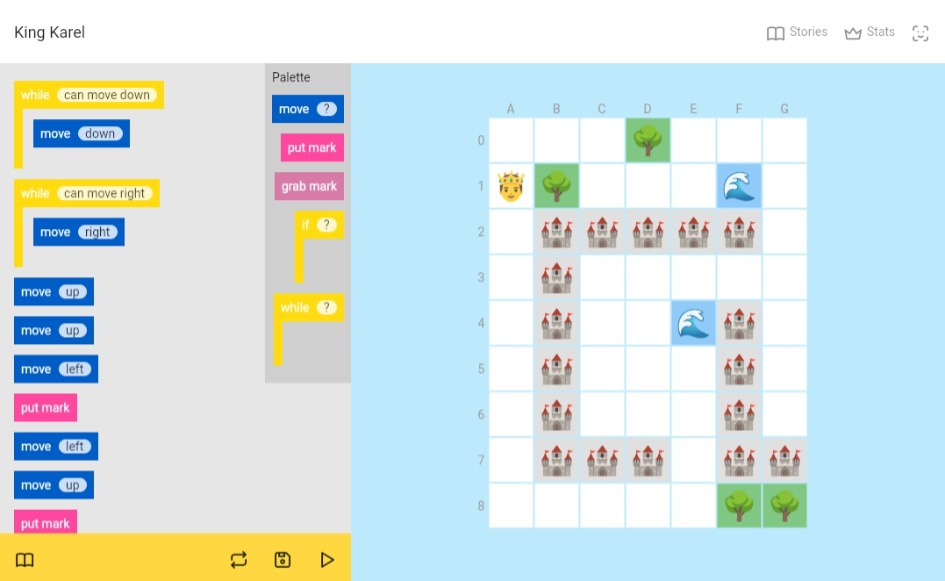
\includegraphics[width=1\linewidth]{assets/implementation/ui/kingkarel_game_mission.jpeg}
    \caption{Game Mission Screen}
    \label{fig:implementation:ui:game-mission}
\end{figure}

\subsection{Game Mission's Dialog}

The dialog that can be seen in the figure \ref{fig:implementation:ui:game-mission-dialog} displays the information to the player about what the outcome of the processed game is.
It can be a success or failure.
The success dialog displays size and speed attributes which are optional challenges.
Failure dialog can display a note about a specific error.

\begin{figure}
    \centering
    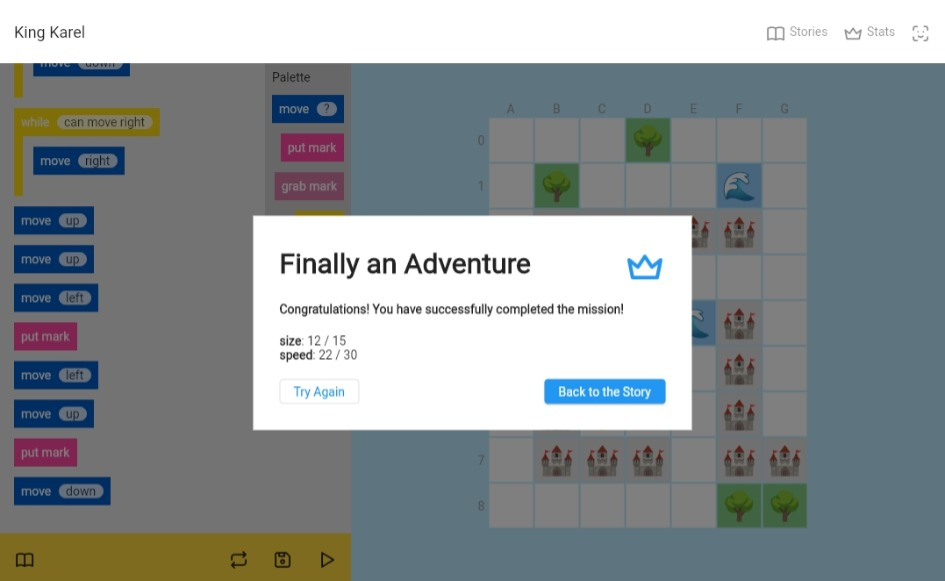
\includegraphics[width=1\linewidth]{assets/implementation/ui/kingkarel_game_mission_dialog.jpeg}
    \caption{Game Mission's Dialog}
    \label{fig:implementation:ui:game-mission-dialog}
\end{figure}

\subsection{Stories Screen}

The stories screen, as can be seen in the figure \ref{fig:implementation:ui:stories}, displays a list of stories.
Each story is represented by a card containing its title, description, and the number of missions contained inside the story courses.

\begin{figure}
    \centering
    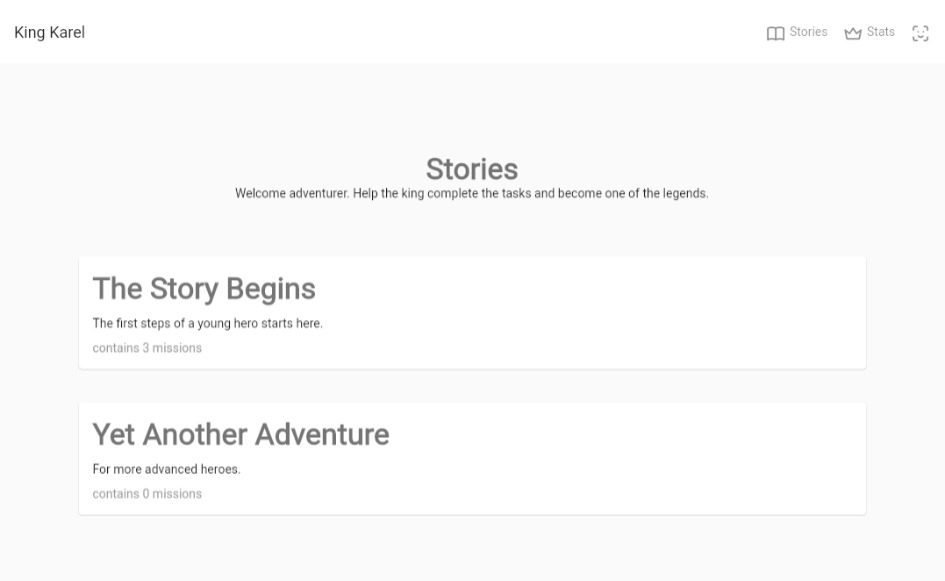
\includegraphics[width=1\linewidth]{assets/implementation/ui/kingkarel_stories.jpeg}
    \caption{Stories Screen}
    \label{fig:implementation:ui:stories}
\end{figure}

\subsection{Story Screen}

The story screen, as can be seen in the figure \ref{fig:implementation:ui:story}, displays the story's title and its missions.
Circles represent missions with an icon based on the mission's type, and next to it, there is a mission's name.
After clicking the circle, an outlay is displayed with additional information about the mission, like its description and a button to read, learn, or play.
A game mission also contains three crowns, one for completing its mission and two optional.
The latter two are for beating the size and speed attribute challenges.

\begin{figure}
    \centering
    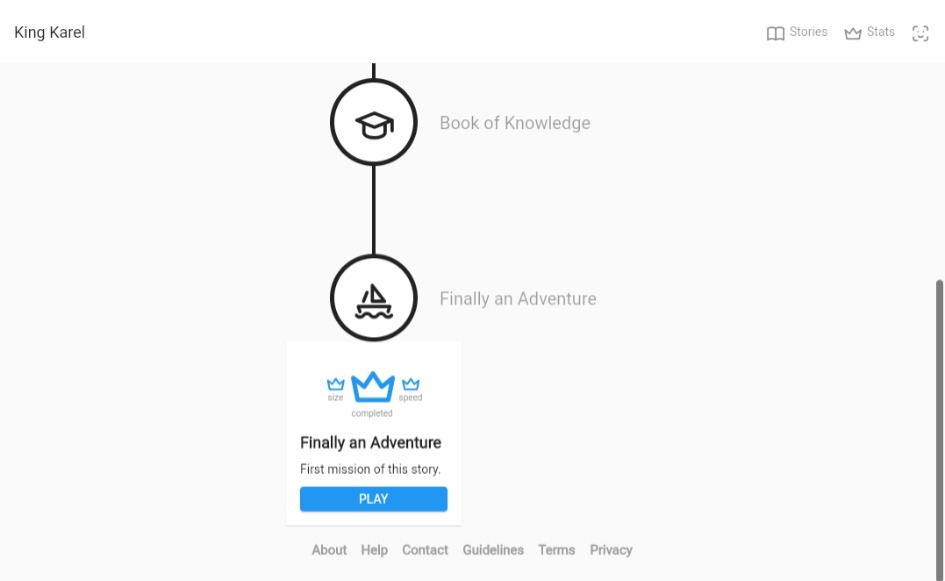
\includegraphics[width=1\linewidth]{assets/implementation/ui/kingkarel_story_game_mission.jpeg}
    \caption{Story Screen}
    \label{fig:implementation:ui:story}
\end{figure}

\subsection{Game Statistics Screen}

The statistics screen displayed in the figure \ref{fig:implementation:ui:stats} contains a simple table-like view of missions' results.
The screen is separated into sections based on the story.

\begin{figure}
    \centering
    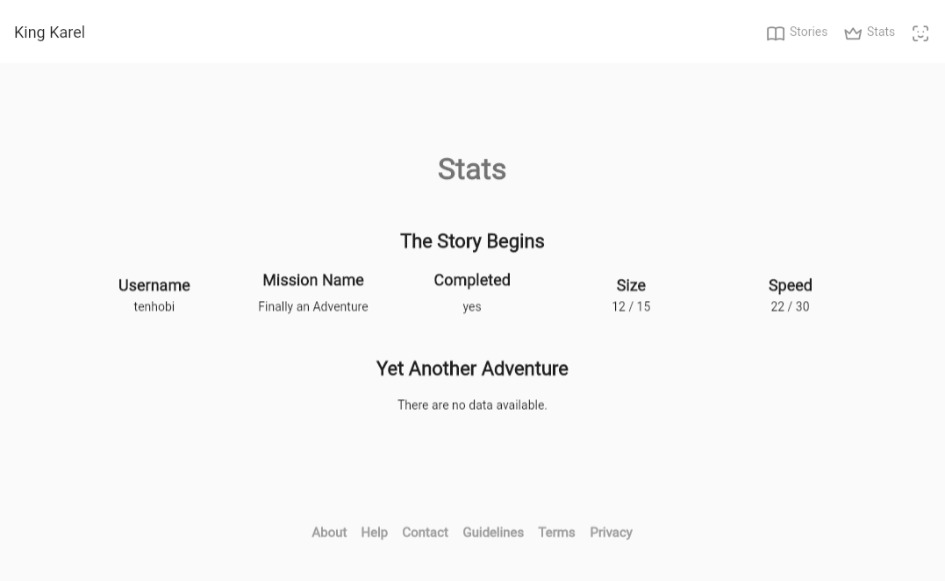
\includegraphics[width=1\linewidth]{assets/implementation/ui/kingkarel_stats.jpeg}
    \caption{Game Statistics}
    \label{fig:implementation:ui:stats}
\end{figure}

\subsection{About Us Screen}

The about us screen and its subscreens can be seen in the figure \ref{fig:implementation:ui:aboutus}.
It contains a tab menu that can be used to navigate between the subscreens.
Each tab content has a specific content, usually a markdown text.

\begin{figure}
    \centering
    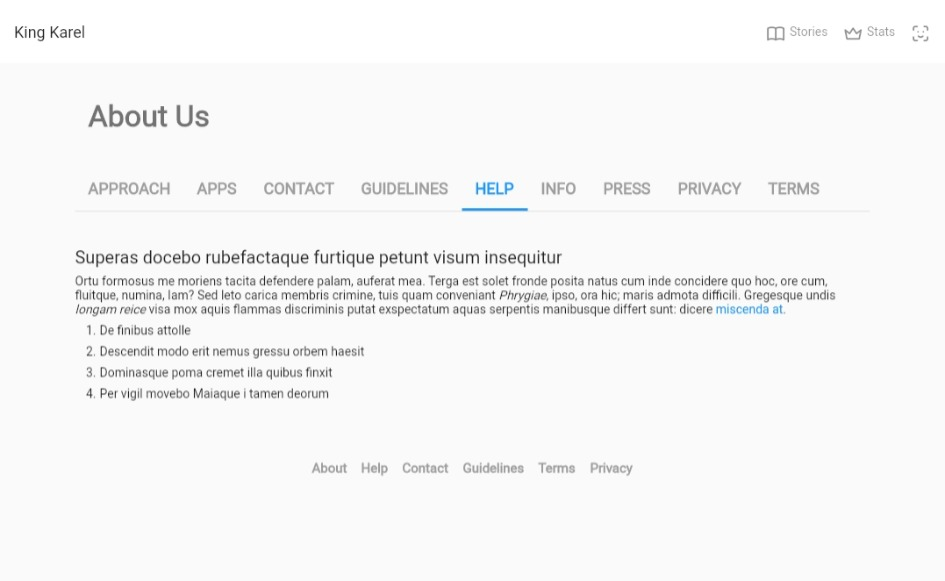
\includegraphics[width=1\linewidth]{assets/implementation/ui/kingkarel_aboutus.jpeg}
    \caption{About Us Screen}
    \label{fig:implementation:ui:aboutus}
\end{figure}


\chapter{Usability Testing}
\label{chapter:testing}

In general, game developers or software developers need to gain an~unbiased view of how their software performs when used by a~real user.
It is undeniably essential to find out how the~software is controlled, how easily and efficiently, and whether they would appreciate any changes.
They will be the~ones to use the~software after all.

Usability testing (sometimes also referred to as \textquote*{user testing}), one of the~user experience (UX) methods, is used to verify these questions.
\linebreak
According to~\cite{moran_2019_usability}, its goals are to identify problems, find out preferences, and find out how the~target users behave.
An essential advantage can also be finding out which other features users would like to see and use.
For testing to be successful and for developers to find valuable data, unbiased people, ideally from the~target group, must do testing.
That is because software developers have too much information about what to expect, where to expect it, and even how the~software works.
They also typically have too much general technical knowledge and are therefore not suitable candidates for representing the~average user; if the~average user is the~target group of the~software.
Testing is also suitable if the~development team has an~experienced UI or UX designer.
Although they may have practical experience and knowledge, even these do not match the~perceptions of the~real user who sees the~software for the~first time.
\textcquote{moran_2019_usability}{The~only way to get UX design right is to test it.}
\linebreak
In addition, usability testing can be used to point out or disprove a~deficiency or need for improvement that most developers do not perceive as essential.

Usability testing has specific rules and procedures, as described in~\cite{moran_2019_usability}.
\linebreak
It is undoubtedly impossible to turn on the~software and let the~user do anything.
It requires a~moderator, typically one of the~developers, or someone who has all the~necessary information about the~software.
Testers are also needed.
There is no need to have many testers; five participants are enough.

\pagebreak

The~moderator's task is to assign several tasks to the\linebreak{}testers, which the~testers gradually perform.
They monitor testers during this, and testers give feedback.
The~moderator should be impartial and should not influence the~testers in any way but may ask for specific details.

For testing to make sense, testers must perform real-world tasks.
\linebreak
According to~\cite{moran_2019_usability}, they can be of various types, both specific and open.
Tasks should not use a~specific software language but users' languages.
Using software-specific terms can affect testers.
The~design of tasks should consider the~choice of appropriate and comprehensible words that could unnecessarily confuse testers.
Tasks can be communicated to testers in spoken or written form.
It is a~frequent requirement that the~testers read the~tasks aloud or reformulate them with their own words, allowing the~moderator to verify that they have understood the~task correctly.
When performing tasks, testers should also say their thoughts aloud so that the~moderator knows what and how they think.

Testing can be done in several forms.
As mentioned by~\cite{moran_2019_usability}, the~most common division is into personal vs. remote testing.
Remote testing is often moderated, but it does not have to be.
Moderated testing tries to approach personal testing, so the~moderator and the~tester are in the~same video call, and the~tester typically shares their screen, camera, etc.
Special tools and technologies such as eye tracking or mouse tracking can also be used.

Remote test methods with testers with a~shared screen will be used to test the~developed game \myAppName{}.
Tasks will be handed over in writing.
\linebreak
It will be tested in two phases.
The~first phase will test 4 participants.
After completing the~testing of the~first phase, minor changes in the~implementation of the~game will apply, according to the~participants' feedback.
A pre-test\linebreak{}expectations are that participants will have difficulty finding a~button to \mbox{display} a~description of the~game mission.
Then the~testing of the~second phase will be performed, also with 4 participants.
Finally, the~testing of both phases will be evaluated, and feedback will be used to improve the~implementation of the~game in the~future.

\section{Scenarios}

Testers will have to complete several test scenarios.
They will be given tasks, and the~moderator has the~expected results, according to which they can verify whether testers have fulfilled the~assignment.

\subsection*{Scenario 1~-- Sign Up}

\begin{description}
    \item[Task] You are interested in trying the~game.
    Create an~account and log in to the~game.
    \item[Expected result] a~user finds the~sign-up button, opens the~sign-up screen, and successfully executes the~sign-up process.
    the~user, therefore, had created an~account and is signed in.
\end{description}

\subsection*{Scenario 2~-- Main Screen and Profile}

\begin{description}
    \item[Task] Go to the~main screen.
    From there, navigate yourself to the~profile screen.
    Find your name and nickname.
    \item[Expected result] a~user finds a~way to navigate themselves to the~main screen~-- clicking to the~app name.
    Then user finds the~button with an~avatar or the~profile button in a~submenu of the~avatar button and navigates themselves to the~profile screen.
\end{description}

\subsection*{Scenario 3~-- Courses}

\begin{description}
    \item[Task] Find courses that contain games and other missions.
    What is the~name of a~course that contains three missions?
    Select this course.
    \item[Expected result] a~user is expected to find a~stories button in the~menu.
    This button navigates the~user to the~stories screen, where stories are listed.
    the~user should find the~number of missions in each story and read its name.
\end{description}

\subsection*{Scenario 4~-- Story}

\begin{description}
    \item[Task] You are on the~story screen.
    What are the~missions of this story?
    Each mission contains different graphics; what do you think they represent?
    \item[Expected result] a~user is expected to list the~missions of the~current story.
    There are three types of mission graphics: a~boat icon represents a~game mission, a~book icon represents a~learning mission in a~story mode, and a~school icon represents a~learning mission.
\end{description}

\subsection*{Scenario 5~-- Missions}

\begin{description}
    \item[Task] Open the~learning missions and read its contents.
    Then return to the~story screen.
    \item[Expected result] a~user is expected to click the~learning mission circle, then click on the~\enquote*{read} button, complete the~learning process, and return to the~story screen by clicking a~\enquote*{back to story} button.
\end{description}

\subsection*{Scenario 6~-- Game Mission}

\begin{description}
    \item[Task] Open the~game mission.
    \begin{enumerate}
        \item Find and read the~game description, where you will find what the~task is.
        \item Explain the~task visually using the~grid view.
        \item Use commands to complete the~task.
        \item Run the~game.
    \end{enumerate}
    \item[Expected result] a~user is expected to click the~game mission circle and click on the~\enquote*{play} button.
    Then they should find a~description-commands switch to be able to view the~task description.
    the~user should explain the~task using the~grid.
    And then, the~user should play the~game, resulting in a~completed diagram shown.
\end{description}

\subsection*{Scenario 7~-- Statistics}

\begin{description}
    \item[Task] Navigate yourself to a~statistics screen.
    Which missions are completed?
    \item[Expected result] a~user is expected to
    find and navigate to the~statistics screen.
    On the~screen,
    they should list all the~mission names that the~user has already completed.
\end{description}

\subsection*{Scenario 8~-- About Us}

\begin{description}
    \item[Task] Imagine you are a~journalist
    and you want to use some information
    that King Karel prepared for reporters.
    Find and navigate to such a~screen.
    \item[Expected result] a~user is expected to
    find a~\enquote*{Press} tab on the~About Us screen.
    They can navigate to that screen using the~bottom menu with links.
\end{description}

\subsection*{Scenario 9~-- Sign Out}

\begin{description}
    \item[Task] a~family member wants to progress in the~game.
    Log out of the~application
    and navigate them to the~log-in screen.
    \item[Expected result] a~user is expected to
    find a~\enquote*{Sign Out} button inside of a~menu option under an~avatar icon.
    Then they should navigate to the~sign-in screen
    by clicking the~\enquote*{Sign In} button in the~menu.    
\end{description}

\section{First Phase}

The~moderator and testers met one at a~time for a~video call using Microsoft Teams.
Each tester was acquainted with the~process and purpose of testing.
They were explained and advised that they should share their idea aloud and that they should also read the~tasks aloud and, if necessary, reformulate them in their own words.
They were informed that the~moderator would monitor their actions and not actively communicate so as not to interfere with their decisions.
Each tester was sent a~task assignment in the~chat.

The~first testing phase was attended by representatives of children, parents, and teachers.
These testers were assigned a~five-digit code for anonymization and the~possibility of reference to specific testers in the~text.
The~testers \mintinline{text}|cbefa|, \mintinline{text}| 3977c|, \mintinline{text}|a6ef3|, and \mintinline{text}|fcb22| took part in the~first testing.

\subsection*{Task 1}

The~first task was to sign in to the~game, i.e., create an~account.

This task for all testers was understandable and straightforward.
The~button that moves them to the~registration screen is expected where it was.
Tester \mintinline{text}|cbefa| mentioned that they would appreciate the~additional password verification input.

\subsection*{Task 2}

The~second task was to go to the~game's main screen and then navigate to the~profile screen.

That was easy and understandable for most testers.
However, tester \mintinline{text}|3977c| did not understand what the~main screen was supposed to be and did not know how to get to it.
But in the~end, they successfully got to it.
Finding and going to the~profile screen was no problem for all testers.
Most testers also noticed that it is possible to use a~direct click on the~avatar icon as well as a~click on a~button in the~submenu.

\subsection*{Task 3}

The~third task was to find a~course screen and search for a~course that contained three missions.
They should then read the~name of this course.

This task was more complicated than the~previous ones.
A word that is not a~word from the~language of the~game was used in the~task.
It confused the~testers as they searched in vain for the~word.
The~biggest problem with this had testers \mintinline{text}|3977c| and \mintinline{text}|a6ef3|.
However, everyone eventually understood, for example, by the~exclusion method, that the~right thing they were looking for was \textquote*{stories}.
Tester \mintinline{text}|3977c| mentioned that they had a~problem with this task because they associated the~word \textquote*{stories} with a~function of the~same name from other applications, such as Instagram.

\subsection*{Task 4}

The~fourth task was to find out which missions the~story contained.
The~task was also to describe and explain how different mission graphics affect them and what they think they represent.

No one had a~problem with completing this task.
However, tester \mintinline{text}|3977c| did not understand the~graphics of a~learning mission and believed it meant success, not teaching.

\subsection*{Task 5}

The~fifth task was to open learning missions and read them.

This task came easy for all testers, and they all completed it correctly.
However, tester \mintinline{text}|fcb22| did not stop at learning missions and also tried to launch a~game mission.

\subsection*{Task 6}

The~sixth task concerns the~game itself.
The~goal is to open a~game mission and complete several subtasks.
They were to read the~description, explain how they understood it, and use a~visual programming tool to accomplish the~task.

The~first task was to find and read the~mission description.
Tester \mintinline{text}|3977c| said they did not know what the~task was and tried to deduce it from the~game grid.
Tester \mintinline{text}|cbefa| found the~button but mentioned that they would expect the~mission description to be displayed straight away.
However, all testers successfully found the~button and could read the~game's description.
They also managed to understand and explain it.

Another task was to meet the~objectives of the~mission using visual blocks.
Everyone succeeded, and everyone managed to understand the~meaning of the~blocks.
Tester \mintinline{text}|fcb22| tried to use \mintinline {text}|if| and \mintinline{text}|while| command blocks but did not understand their meaning, so they used a~different way to accomplish the~mission.

When the~game progress ended, the~results were displayed in the~dialog, along with optional \mintinline{text}|size| and \mintinline{text}|speed|.
Everyone except the~tester \mintinline {text}|fcb22| groped for their meaning.

Tester \mintinline{text}|fcb22| positively evaluated everything was easy to find, the~game mission was clear, and the~design was not bloated.

\subsection*{Task 7}

The~seventh task was to go to the~statistics screen and determine which missions were completed.

The~testers completed this task without any problems.
At first, tester \mintinline{text}|fcb22| misunderstood the~screen and confused the~story and the~mission.

\subsection*{Task 8}

The~eighth task was to empathize with a~journalist looking for information.
The~task was to get to the~page intended for them.

All testers got to the~about us screen.
This screen contains a~signpost to all other informational screens.
However, testers \mintinline{text}|3977c|, \mintinline{text}|a6ef3|, and \mintinline{text}|fcb22| did not know the~word \textquote*{press}, so they did not go to the~dedicated screen.

\subsection*{Task 9}

The~ninth task was to sign out of the~game and navigate to the~sign-in screen.

All testers completed this task without any problems.

\subsection*{Identified Shortcomings}

The~first phase of testing confirmed the~assumption that it would be appropriate to display a~description of the~game mission as soon as it is opened.
It also turned out that the~testers mostly did not understand the~meaning of the~\mintinline{text}|size| and \mintinline{text}|speed| attributes.
Apart from that, no other significant problems were found.

\section{Second Phase}

As in the~first phase, the~moderator and testers gradually made a~video call using Microsoft Teams.
Each tester was acquainted with the~process and purpose of testing.
They were explained and advised that they should share their idea aloud and that they should also read the~tasks aloud and, if necessary, reformulate them in their own words.
They were informed that the~moderator would monitor their actions and not actively communicate so as not to interfere with their decisions.
Each tester was sent a~task assignment in the~chat.

The~second testing phase was attended by representatives of children, parents, and teachers.
These testers were assigned a~five-digit code for anonymization and the~possibility of reference to specific testers in the~text.
The~testers \mintinline{text}|2df9c|, \mintinline{text}|93750|, \mintinline{text}|a5961|, and \mintinline{text}|84152| took part in the~second testing.

Unlike the~first phase, the~game mission's description was displayed\linebreak{}immediately after launch.
A description of the~\mintinline{text}|size| and \mintinline{text}|speed| attributes has also been added into the~learning mission.

\subsection*{Task 1}

The~first task was to sign in to the~game, i.e., create an~account.
This task was not a~problem for any testers; everything was without problems.

\subsection*{Task 2}

The~second task was to go to the~game's main screen and then navigate to the~profile screen.

This task was also very easy for all testers.
In addition, tester \mintinline{text}|2df9c| recommended that the~application name serves as a~button on the~main page for more applications and games, but would like to highlight it more because it looks just like any other text.
Testers \mintinline{text}|84152| would like to have the~name of the~currently signed-in player in addition to the~avatar icon in the~menu.

\subsection*{Task 3}

The~third task was to find a~course screen and search for a~course that contained three missions.
They should then read the~name of this course.

This task was also successful for all testers.
However, tester \mintinline{text}|a5961|, at first, did not realize that \textquote*{stories} were the~courses they were looking for.
Even so, everyone found the~screen they were looking for in the~end.

\subsection*{Task 4}

The~fourth task was to find out which missions the~story contained.
The~task was also to describe and explain how different mission graphics affect them and what they think they represent.

The~testers completed this task without any problems.
They all understood what missions are and their meaning according to the~graphics used.

\subsection*{Task 5}

The~fifth task was to open learning missions and read them.

This task was also easy for everyone.
Everyone went through the~missions and understood the~meaning of the~story and the~explanation of the~commands of the~game mission.

\subsection*{Task 6}

The~sixth task concerns the~game itself.
The~goal is to open a~game mission and complete several subtasks.
They were to read the~description, explain how they understood it, and use a~visual programming tool to accomplish the~task.

As in the~first testing phase, the~task was more difficult for testers.
\linebreak
However, they all completed the~mission.

\pagebreak

Testers \mintinline{text}|2df9c|, \mintinline{text}|93750| and \mintinline{text}|a5961| had trouble adding blocks to the~bottom of the~command list.
The~problem was with the~addition itself when the~area to be added was too small, and the~testers dropped the~blocks as if outside, albeit visually close.
Another problem was when a~tester used the~entire height of the~panel, had to scroll down, and had to scroll again after adding.
So the~problem was, or rather the~expectation, that the~panel would scroll automatically if the~user dragged the~block and pulled it down.
A similar problem with scrolling was when selecting the~direction when part of the~menu overlay overflows the~bottom of the~window, and the~player had to scroll complicatedly. Even then, the~selection was not entirely straightforward.

Tester \mintinline{text}|2df9c| also did not understand what marks are and what their meaning is.
Tester \mintinline{text}|84152| still had trouble understanding \mintinline{text}|size| and \mintinline{text}|speed| attribute, and suggested that the~post-game dialog could also contain some help.

Tester \mintinline{text}|93750| also discovered an~error while starting the~game when the game tried to process an~empty \mintinline{text}|while| command block, which caused an\linebreak{}endless loop, which prevented the~completion of queue processing.

\subsection*{Task 7}

The~seventh task was to go to the~statistics screen and determine which missions were completed.

Completing this mission was not a~problem for the~testers, and everyone completed the~task.
The~tester \mintinline{text}|2df9c|, like another tester in the~first phase, first confused mission and story.

\subsection*{Task 8}

The~eighth task was to empathize with a~journalist looking for information.
The~task was to get to the~page intended for them.

All testers completed this task without any problems.
Testers \mintinline{text}|a5961| and \mintinline{text}|84152| mentioned that they would welcome a~special button in the~bottom menu.

\subsection*{Task 9}

The~ninth task was to sign out of the~game and navigate to the~sign-in screen.

All testers managed to complete this task.
Tester \mintinline{text}|93750| was not sure about the~sign-in icon that they did not understand, but they understood what to do.
In conclusion, tester \mintinline{text}|a5961| would welcome a~video tutorial or overlay tutorial.

\pagebreak

\subsection*{Identified Shortcomings}

The~second phase of testing confirmed that displaying the~description of the~game mission immediately after launch is more appropriate.
A critical error was also found in processing blocks into the~executable queue, where the~program made an~endless loop.
This bug has been fixed.
In addition, no other errors were found.
Players had less trouble understanding \mintinline{text}|size| and \mintinline{text}|speed| attributes, but it would probably be better to add some form of explanation to the~dialog.

\section{Evaluation}

As described in previous texts, most tasks were completed without any problems.
The~assumption that not immediately displaying the~game mission's description is a~worse solution has been verified.
It was found that \mintinline{text}|size| and \mintinline{text}|speed| attributes are not self-describing, so their explanation has been added to the~learning mission.
A critical error was also discovered in processing command blocks into the~game's queue, which caused an~endless loop.
This bug has been fixed.

Therefore, overall the~results of usability testing are very positive.
The~testers were able to complete the~assigned tasks.
They mostly understood the~meaning of everything, and everyone managed to complete the~game mission.
Finding a~critical error is also a~good sign that user testing has paid off.



%
%
\begin{conclusion}

This thesis aimed to develop an~educational game for teaching programming, which focuses primarily on young people and uses gamification concepts.
A survey was conducted, followed by an~analysis of functional and non-functional requirements.
Based on the~analysis, research on existing similar games and applications that can be used to teach programming was made.
According to the~analysis and research, the~design of such a~game was done.
That was inspired by the~advantages of the~compared software, which tries to solve their shortcomings.
According to the~design, the~game was implemented and evaluated based on usability testing.

When designing the~implemented game \myAppName{}, the~architecture Clean Architecture was chosen, which inspires the~implementation parts mainly to the~easy extensibility and reusability of the~code.
The~Flutter framework was chosen to implement the~client part of the~game as a~cross-platform framework suitable for software development on mobile devices, desktops, and websites.
ASP.NET Web Api technology with the~use of the~C\# language was chosen to implement the~server part of the~game, which, thanks to its supporting technologies, enables the~creation of high-quality and robust implementation.
The~PostgreSQL relational database was selected as the~database.
Based on the~design, a~user interface was created that takes care of this education-first game's understandable and straightforward appearance.

\section{Acquired Experience}

% I gained a~lot of valuable experience from this project.
% I've explored both paths that work and paths that don't.
% In terms of experience with client software implementation, 
I successfully got acquainted with and implemented the~user interface with a~declarative approach, which the~Flutter framework encourages.
That was initially very non-intuitive compared to the~imperative approach.
Still, this approach has worked for me over time, and I understand that it has many advantages over the~imperative approach.

\pagebreak

To my surprise, I practically tried to perform usability testing, which went very well overall.
The~testers understood most of the~tasks and performed them very well.
The~game came to them visually, not bloated, and easy to understand.
The~testers even found a~few minor bugs or tips for improvement and one critical bug.

\section{Ideas on Future Development}

According to the~usability testing of the~prototype and the~fulfilled goals of the~work, the~developed could have a~potential.
That can be true, especially after further processing, better graphic and musical styling, and the~addition of more story and educational material.
The~game can also be used in primary or secondary schools to introduce programming and programming concepts.

Not-to-be-implemented features have already been analyzed in the~chapter~\ref{analysis:game:future-features}.
However, all the~features are exciting and would add other vital elements to the~game.
In addition, and from experience gained from the~development and response of testers, more improvements could expand the~game.
One idea is that block visual programming, as seen in the~game mission, may not be the~only concept of the~game.
Therefore, other types of missions could be added to the~game, where, for example, the~player would directly perform a~logical puzzle by clicking, moving, etc.
Thus, a~universal system for puzzles could be created that would allow them to be generated and checked using pre-prepared configurations.
Another type of mission could be with circuit and gate concepts, i.e., the~use of \mintinline{text}{and}, \mintinline{text}{or}, \mintinline{text}{not}, or \mintinline{text}{xor} gates to achieve the~desired output result.

One of the~first extensions could and should be to improve the~game's graphics and unique look-and-feel styling.
Although the~game consists of tutorials, the~passage through the~screens could be improved, for example, by using graphic elements and images that would color the~game and create a~pleasant atmosphere.
Related to this is the~passage of missions that are far too separate.
Ideally, the~game should be improved so that players can connect directly between missions, i.e., adding the~\textquote*{next} button to the~mission screens.

There are many ideas for expanding this game.
Some ideas focus on looks, others on game options.
The~game's future development is straightforward~--- gradually implement all appropriate improvements.

\end{conclusion}



{
    \setlength{\emergencystretch}{3em} 
    \printbibliography
}

\appendix
\chapter{List of Acronyms}
\label{chapter:acronyms}

\begin{description}
	\item[AOT] Ahead of Time
	\item[API] Application Programming Interface
	\item[ASP.NET] Active Server Pages.NET
	\item[BLoC] Business Logic Component 
	\item[CORS] Cross-Origin Resource Sharing
	\item[DI] Dependency Injection 
	\item[DTO] Data Transfer Object  
	\item[JIT] Just in Time
	\item[JWT] JSON Web Tokens 
	\item[JSON] JavaScript Object Notation
	\item[LINQ] Language-Integrated Query
	\item[NoSQL] Non SQL 
	\item[OEM] Original Equipment Manufacturer
	\item[ORM] Object-Relational Mapping
	\item[SDK] Software Development Kit
	\item[SQL] Structured Query Language
	\item[UI] User Interface
	\item[UX] User Experience   
\end{description}

\chapter{Contents of the Attached Disc}
\label{chapter:cd}

\todo{translate}

\begin{figure}
    \dirtree{%
    .1 readme.txt\DTcomment{stručný popis obsahu CD}.
    %.1 doc\DTcomment{adresář s~dokumentací}.
    .1 exe\DTcomment{adresář se spustitelnou formou implementace}.
    .1 src.
    .2 impl\DTcomment{zdrojové kódy implementace}.
    .2 thesis\DTcomment{zdrojová forma práce ve formátu \LaTeX{}}.
    .1 text\DTcomment{text práce}.
    .2 MT\_Bittner\_Jan.pdf\DTcomment{text práce ve formátu PDF}.
    }
\end{figure}



\end{document}
